\noindent
This chapter is the first study to reveal the dynamics of time-varying oligopsonistic competition and storage adoption, and their impacts on smallholder farmers' welfare. While existing research explores storage incentives like risk preferences and trading costs, it overlooks the advantages of quality-preserving technologies for accessing markets over time that might vary in their competitiveness. Cold storage adoption, especially for semi-perishable crops, helps farmers overcome trading-time limitations. By constructing a two-period post-harvest management model for a storable cash crop, I find that temporal changes in buyer power alone can suffice for farmers to benefit from storage. This work has broader relevance to settings with multiple input suppliers selling to a limited set of traders involved in market division and price fixing over time.

%--------------------------------------------------------%
\section{Introduction}
\noindent    
Buyer power arises from the immobility of certain factor inputs that, in the short run, are largely ``captive'' to a limited set of buyers. While spatial immobility has been extensively explored in the literature, the impact of changes in temporal immobility on bargaining dynamics remains underexamined. This gap is particularly relevant in agricultural markets, where products are typically somewhat perishable, and proper storage plays a critical role in the supply chain.


To the best of our knowledge, this study is the first to unveil the interplay of farmers' (sellers') storage adoption in the presence of time-varying competition in the procurement market. Without the adoption of storage, smallholder farmers who cultivate crops that spoil quickly face limitations in their trading options, as they can only sell their produce locally at harvest time because they typically lack access to trucks or other transportation equipment, preventing them from accessing distant selling locations. But if they were equipped with advanced storage technology, they would be able to seek out a higher local price brought from more competitive market conditions among middlemen in the later periods, as shown in Figure \ref{Figure: Demo}.

\begin{figure}[ht!]
\centering
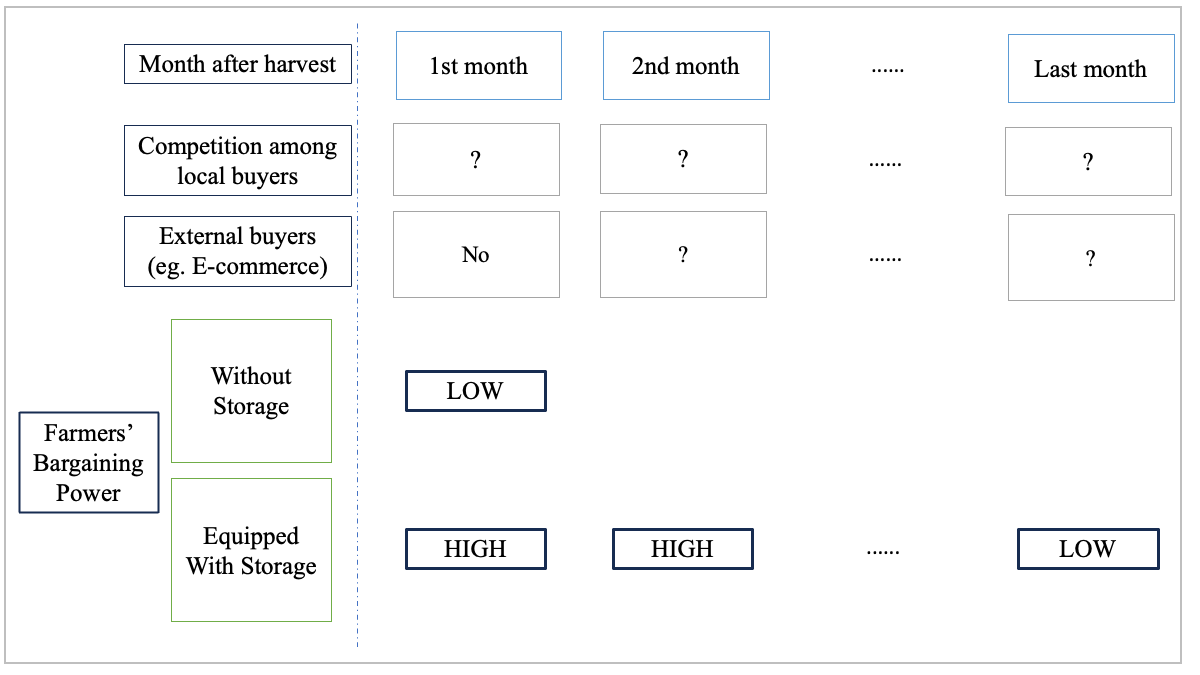
\includegraphics[width=1\textwidth]{figures/graphic_demo.png}
\caption{Extended Marketing Opportunities from Storage Adoption}
\label{Figure: Demo}
\end{figure}

Specifically, farmers could potentially benefit from increased competition in the oligopsonistic market through two sources. Firstly, the presence of different intermediaries in the village at various times can create fluctuating levels of competition on a monthly or even weekly basis.\footnote{In this chapter, the terms middlemen, field buyers, intermediaries, and traders will be used interchangeably to refer to a group of buyers who directly purchase fresh apples from farmers. These buyers play a crucial role in the supply chain by acting as the initial link between farmers and the downstream market. They typically visit orchards, negotiate prices with farmers, and handle the immediate procurement of apples. Their role may also include transporting apples to wholesale markets, processing facilities, or exporters, depending on the supply chain dynamics. Regardless of the specific term used, all these buyers share the common function of directly sourcing apples from farmers and selling them downstream to wholesalers, retailers, and processors.}  Secondly, farmers with storage can tap into additional distribution channels such as e-commerce and direct selling, which differ from the conventional middlemen-dominated system. By doing so, they can introduce external participants into the oligopsonistic market at the farm gate at different time nodes. 

I develop a conceptual framework to explore how smallholder farmers can adopt cold storage to potentially exploit the time-varying buyer power of middlemen. It considers a simplified two-period scenario in a developing country, where farmers sell a specific cash crop to middlemen who visit local villages to procure the farm product. The model incorporates a storage-decision process, wherein farmers, observing farm-gate prices at harvest, decide whether to sell or store their crops.

The outcomes of this study hold substantial implications for policymakers and farmers alike. By exploring the dynamics of time-varying oligopsony levels, the research aims to demonstrate the potential benefits of storage facilities for smallholder producers. In a broader context, the findings suggest that embracing storage adoption could provide farmers with an effective alternative to combat anti-competitive practices like buyer collusion and market allocations and avoid more intrusive measures in markets, such as direct government intervention.





\section{Base Model}
\noindent I develop a two-period dynamic model to analyze how smallholder farmers strategically utilize storage in response to time-varying buyer power exerted by middlemen. The model is set in a rural area of a developing country, where farmers market a cash crop to itinerant traders. Harvest quantity is treated as exogenous, and the analysis focuses exclusively on farmers' storage and sales decisions within a single crop cycle. To sharpen focus on the impact of market structure and trading dynamics, product quality is assumed homogeneous across farmers.

Farmers exhibit risk preferences ranging from risk neutrality to moderate risk aversion and value own consumption at market prices. Each farmer is represented by a von Neumann-Morgenstern utility function,\footnote{An alternative mean-variance framework, presented in Appendix~\ref{Appendix: mean-variance approach}, yields similar insights. However, due to limited empirical guidance on calibrating the risk aversion coefficient within agricultural supply chains for the mean-variance framework, my primary analysis relies on the expected utility framework.} $U_i(\pi_i)$, with $U_i' > 0$ and $U_i'' \leq 0$, where $\pi_i$ is the farmer's net income from crop sales. Farmers aim to maximize the expected utility of income across two trading periods.

The central decision is determining the proportion of the crop stored at harvest, denoted by $s \in [0,1]$. This choice is made under uncertainty about future market conditions, specifically future buyer power dynamics in the subsequent trading period. I will represent buyer power in each period $t$ by the parameter $\theta_t$ and will later show that I can bound $\theta_t$ in the unit interval.

In the initial trading period, farmers observe farm-gate price offers from middlemen. Based on the frequency and magnitudes of these offers, farmers infer the current buyer power. represented by $\theta_1$. Greater competition among buyers, characterized by lower $\theta_1$, correlates with higher farm-gate prices, $p_1$. Anticipating continuity in the inverse relationship between buyer power and prices across periods, farmers strategically allocate harvest between immediate sale and storage, incorporating expectations about future competition, captured by the random variable $\theta_2$.

Temporal demand variations downstream, such as seasonal consumption shifts, are presumed to be fully internalized by the market as a whole, including both farmers and intermediaries. Since intermediaries may engage in storage, anticipated demand fluctuations over the marketing season should already be reflected in the prices they offer at harvest. Accordingly, buyer power remains the primary source of intertemporal price variability in this model.

The model assumes symmetric information and negligible transaction costs in each trading period, ensuring farmers have complete and instantaneous access to prevailing farm-gate prices.

Formally, each farmer seeks to maximize expected utility over two trading periods by selecting storage share $s \in [0,1]$. Given a normalized harvest quantity $q = 1$, the optimization problem is:
\begin{equation}
\label{eq:starting objective}
\max_{s \in [0,1]} \mathbb{E} \left(U\left[ (1 - s) p_1 + s \cdot p_{2,\text{net}} \right]\right).
\end{equation}
where $p_1$ is the farm-gate price at harvest and $p_{2,\text{net}}$ is the second-period price adjusted for storage costs.



\subsection{Middlemen Market Structure and Farm-Gate Price Formation} \label{Section: Middlemen Market Structure and Farm-Gate Price Formation}
\noindent To analyze farmers' strategic use of storage as a form of intertemporal bargaining, it is essential to model farm-gate price formation in a manner that flexibly incorporates the degree of competition among middlemen.

I adopt the \textit{Flexible Oligopoly/Oligopsony Market (\textit{FOOM})} framework to model farm-gate pricing as a function of buyer market power. Under the assumption that downstream markets, wholesale or retail, where traders sell the farm products they procure, are perfectly competitive, the farm-gate price $p_{f,t}$ in each period $t$ is determined as:
\begin{equation}
p_{f,t} = \frac{p_{r,t} - mc_t}{1 + \frac{\theta_t}{\varepsilon_t}},
\end{equation}
where $p_{r,t}$ is the downstream price and $mc_t$ denotes the buyers' marginal cost in period $t$, $\theta_t$ captures the degree of buyer power in period $t$, and $\varepsilon_t$ represents the farm supply elasticity facing buyers in period $t$.\footnote{For a detailed derivation, see Appendix~\ref{Appendix: Derivation of Farm Price under the FOOM Framework}.}


For simplicity, supposing the downstream price net of marginal cost is constant across periods and normalizing it to unity ($p_{r,t} - mc_t = 1$), the farm-gate price reduces to:
\begin{equation}
p_{f,t} = \frac{\varepsilon_t}{\varepsilon_t + \theta_t}.
\end{equation}


Although total harvest quantity is fixed at the time of the first-period decision, supply in that period remains somewhat elastic due to farmers' ability to store part of their output. In period 2, supply is also elastic, as farmers can divert unsold produce to alternative buyers such as fruit-processing firms. To simplify the analysis while preserving these features, I assume a baseline supply elasticity of $\varepsilon_t = 1$ for both periods. This assumption serves as a plausible starting point and will be relaxed in subsequent analysis. Thus, farm-gate prices reduce further to:
\begin{equation}
p_{f,t} = \frac{1}{1+\theta_t}, \quad \theta_t \in [0,1] \text{ and } t \in \{1,2\},
\label{Eq: price formation by buyer power}
\end{equation}
where $\theta_t=0$ corresponds to perfect competition among buyers and $\theta_t=1$ denotes pure monopsony. Forms of oligopsony competition, such as Cournot competition, are represented by intermediate values of $\theta_t$, with higher values denoting progressively greater departures from competition \citep{karp1996dynamic,sexton2001assessment, saitone2009flexible, hamilton2021joint}.

Assuming farmers believe that this price formation rule persists across periods, period-specific prices are determined as $p_t = \frac{1}{1+\theta_t}, \quad t=1,2$. At harvest time, farmers observe $p_1$ and infer the contemporaneous buyer power, $\theta_1 = \frac{1 - p_1}{p_1}$. They then form expectations about the second-period buyer power, $\theta_2 \in [0,1]$, which is stochastic, and its distribution can be independent or based on the observation of $\theta_1$ under further assumptions. Thus, the second-period price can be expressed as:
\begin{equation}
p_2(\theta_2) = \frac{1}{1+\theta_2} 
\label{Eq: p_2 of buyer power change}
\end{equation}


To incorporate the economic cost of storage--including physical storage expenses, intertemporal discounting, and potential quality deterioration--I define the second-period price in net terms using a storage efficiency parameter $\kappa \in [0,1]$, which captures the overall storability of the commodity. Rather than modeling storage cost as a fixed deduction, I assume that storage frictions reduce the realized price proportionally, so that the farmer receives only a fraction $\kappa$ of the gross second-period price. This formulation captures a broad class of storage frictions, such as spoilage, shrinkage, and financing costs, that scale with the value of the commodity. It also reflects how farmers often perceive post-harvest losses: as a proportional reduction in potential revenue. From an analytical standpoint, the proportional specification preserves tractability under the Constant Relative Risk Aversion (CRRA) preferences, where utility is homogeneous of degree one and sensitive to relative rather than absolute changes in income. Accordingly, I define the net second-period price as:
$$
p_{2,\text{net}}(\theta_2) = \kappa \cdot p_2(\theta_2),
$$
where the gross second-period price remains $p_2(\theta_2) = \frac{1}{1 + \theta_2}$. Thus, the full expression becomes:
$$
p_{2,\text{net}}(\theta_2) = \frac{\kappa}{1 + \theta_2}.
$$
This setup ensures that the incentive to store responds coherently to economic fundamentals while allowing for an intuitive interpretation of $\kappa$: when $\kappa = 0$, the product is perfectly perishable and yields no second-period returns; when $\kappa = 1$, the product is perfectly storable with no loss in value.


In this framework, farmers' intertemporal storage decision critically depends on their expectations about future buyer power, $E[\theta_2]$, which directly shape their expectations of the net second-period price, $E[p_{2,\text{net}}] = E\!\left[\frac{\kappa}{1+\theta_2}\right]$. Since $\theta_2$ is uncertain at the time of harvest, farmers form beliefs about its distribution, potentially informed by first-period buyer conduct ($\theta_1$) or/and past trading experiences. These expectations determine the perceived intertemporal price differential between immediate sale and deferred sale through storage, thereby linking market-structure uncertainty to individual storage incentives.





\subsection{Final Objective Function}

\noindent The economic environment at harvest is summarized in Table~\ref{tab:baseline model parameter table}, capturing both observed and unobserved determinants of the farmer's storage decision over two periods.

\begin{table}[H]
\centering
\caption{Economic Environment at Harvest}
\label{tab:baseline model parameter table}
\begin{tabular}{lll}
\toprule
\textbf{Item} & \textbf{Symbol (units)} & \textbf{Status at Harvest} \\
\midrule
Harvest quantity & $q$ & Known, fixed (normalized to 1) \\
First-period price & $p_1$ & Observed \\
First-period buyer power & $\theta_1 = \frac{1 - p_1}{p_1}$ & Inferred from $p_1$ \\
Second-period buyer power & $\theta_2$ & Stochastic \\
Second-period price & $p_2 = \frac{1}{1 + \theta_2}$ & Derived \\
Storage efficiency factor & $\kappa \in [0,1]$ & Observed \\
Second-period net price & $p_{2,\text{net}} = \frac{\kappa}{1 + \theta_2}$ & Derived \\
CRRA risk aversion & $\gamma \in [0,10]$ & Observed \\
\bottomrule
\end{tabular}
\end{table}

\noindent The farmer allocates a share $s \in [0,1]$ of output to the second-period sale and retains the remainder for immediate sale at price $p_1$. Without a specific assumption on the utility functional form, substituting the expressions for $p_1$ and $p_{2,\text{net}}$, a farmer's maximization problem becomes:
\begin{equation}
\label{eq:final objective}
\max_{s \in [0,1]} \mathbb{E} \left\{U\left[\underbrace{\frac{1-s}{1+\theta_1}}_{\text{First-period income}} + \underbrace{s \cdot \frac{\kappa}{1+\theta_2}}_{\text{Adjusted second-period income}} \right]\right\}.
\end{equation}


\subsection{Risk Neutrality: Closed-Form Solution}
\noindent Under the case of risk neutrality, the utility function becomes linear: $U(\pi) = \pi$. The objective simplifies to:
\begin{equation}
\max_{s \in [0,1]} \; 
(1 - s) \cdot \frac{1}{1 + \theta_1} 
+ 
s \cdot \kappa \cdot \mathbb{E} \left[ \frac{1}{1 + \theta_2} \right].
\end{equation}
The solution simply depends on a comparison of marginal returns:
\begin{equation}
s^*( \gamma = 0) =
\begin{cases}
1 & \text{if } \kappa \cdot \mathbb{E} \left[ \frac{1}{1 + \theta_2} \right] > \frac{1}{1 + \theta_1}, \\
0 & \text{if } \kappa \cdot \mathbb{E} \left[ \frac{1}{1 + \theta_2} \right] < \frac{1}{1 + \theta_1}, \\
\text{any } s \in [0,1] & \text{if equality}.
\end{cases}
\label{Eq: risk-neutrality solution}
\end{equation}

\noindent Under risk neutrality, the farmer evaluates only expected monetary payoff. The decision reduces to a pure binary choice: if the net expected second-period price exceeds the normalized first-period price, then storage is optimal; otherwise, immediate sale dominates. Indifference arises only when the two expected returns are equal.


\subsection{Risk Aversion: Numerical Approach Needed}
\noindent In the presence of risk aversion---that is, when the utility function is strictly concave---analytical solutions to the farmer's maximization problem are generally unattainable. This intractability arises from the fact that risk aversion embeds the random second--period buyer-power parameter, $\theta_2$, inside a nonlinear transformation.  With a strictly concave utility function $U(\cdot)$, the marginal utility term that enters the first-order condition is $U'\!\left[\frac{1-s}{1+\theta_1}+ s\frac{\kappa}{1+\theta_2}\right]$.  Because $s$ appears both outside and inside the expectation, the optimality condition requires solving
$$
\mathbb{E}\!\left\{\,U'\!\Bigl[\cdot\Bigr]\!\left[-\frac{1}{1+\theta_1}+\frac{\kappa}{1+\theta_2}\right]\right\}=0,
$$
which is a Fredholm integral equation. For generic concave $U$ (e.g., CRRA, CARA, or quadratic utility outside the linear range), the integral has no closed-form anti-derivative, because $U'$ must be evaluated at every realization of $\theta_2$ and then averaged over its distribution. Only by imposing knife-edge assumptions---such as risk neutrality ($U''=0$), degenerate $\theta_2$, or special affine-transform utility---does the expectation reduce to an algebraic expression that can be inverted to solve for $s$.

Even when the distribution of $\theta_2$ is simple, analytic integration remains elusive. The ratio $\kappa/(1+\theta_2)$ introduces a hyperbolic term inside $U$, so the composition $U'\circ g(\theta_2)$ usually lacks a primitive.  Consequently, the derivative of the expected utility cannot be written as a finite combination of elementary functions, precluding a closed-form solution for the interior optimum. 

Moreover, the introduction of risk aversion couples the mean and higher-order moments of $\theta_2$ together. The comparative-static effects of skewness or variance on $s^{*}$ therefore enter through higher-order derivatives of $U$, which are inseparable from the integral above.  This dependence further limits traceability.


These complications drive me to employ numerical analysis, specifically, the Monte Carlo evaluation of the expectation, to approximate the optimal storage share $s^{*}$ while respecting the corner constraints $s\in[0,1]$.





\section{Numerical Analysis} \label{Section: Base Model Numerical Analysis}
\noindent To examine how risk preferences and storage efficiency shape farmers' intertemporal marketing decisions under buyer power uncertainty, I numerically solve for the optimal storage share $s^*$ across a range of parameter values. This section describes the simulation design and computational procedure employed to approximate the farmer's decision problem under Constant Relative Risk Aversion (CRRA) utility.


\subsection{Setup and Parameterization}
\noindent Without much loss of generality, a farmer is assumed to observe a moderate level of first-period buyer power $\theta_1 = 0.5$, the midpoint of the support. The choice of $\theta_1 = 0.5$ serves as a representative benchmark rather than a substantive restriction. The objective here is not to analyze the effect of a specific level of contemporaneous buyer power, but to illustrate how changes in the mean and variance of future buyer power, $\theta_2$, around the first-period observation influence farmers' storage incentives. Similar qualitative insights would arise under alternative values of $\theta_1$, as the key mechanism operates through how expectations about $\theta_2$ evolve relative to the observed market condition, rather than through the absolute level of $\theta_1$ itself.


Second-period buyer power $\theta_2$ is stochastic and modeled using Beta distributions bounded on the unit interval $[0,1]$, allowing for flexible skewness and kurtosis while maintaining economically relevant support.

I consider eight distinct Beta distributions defined by a full factorial combination of:
\begin{itemize}
\item \textbf{Four means}: $\mu_{(\theta_2)} \in {0.2,,0.4,,0.5,,0.8}$, and
\item \textbf{Two variances}: $\sigma^2_{(\theta_2)} \in {0.02,,0.05}$, representing low and high uncertainty respectively.
\end{itemize}

For each $(\mu_{(\theta_2)}, \sigma^2_{(\theta_2)})$ pair, the corresponding unique pair of Beta distribution shape parameters $(\alpha, \beta)$ is computed using the standard moment-matching formulas:

$$
\alpha = \mu_{(\theta_2)} \left( \frac{\mu_{(\theta_2)}(1 - \mu_{(\theta_2)})}{\sigma^2_{(\theta_2)}} - 1 \right), \quad
\beta = (1 - \mu_{(\theta_2)}) \left( \frac{\mu_{(\theta_2)}(1 - \mu_{(\theta_2)})}{\sigma^2_{(\theta_2)}} - 1 \right).
$$

I simulate 2,000 independent realizations of $\theta_2$ for each Beta distribution to approximate the expectation operator in the farmer's objective function.




\subsection{Numerical Strategy}
\noindent The computational approach exploits a simplification under risk neutrality ($\gamma = 0$). In this case, the utility function becomes linear and the farmer's decision reduces to the binary rule as shown in Equation~\ref{Eq: risk-neutrality solution}.

For all $\gamma > 0$, I numerically evaluate a farmer's utility under the Constant Relative Risk Aversion (CRRA) functional form:
\begin{equation}
U(\pi)=\left\{\begin{array}{ll}
\frac{\left(\pi^{1-\gamma}-1\right)}{(1-\gamma)} & \text { if } \gamma \neq 1 \\
\ln (\pi) & \text { if } \gamma=1
\end{array},\right.
\label{eq: CRRA}
\end{equation}
where $\gamma$ denotes the coefficient of relative risk aversion, and $\pi$ represents the net income realized over two periods. 

The adoption of the Constant Relative Risk Aversion (CRRA) utility function is supported by both theoretical appeal and empirical evidence. Theoretically, CRRA maintains a constant degree of relative risk aversion across income levels, aligning with microeconomic models of choice under uncertainty. Empirically, panel data studies consistently find that the share of risky assets in household portfolios remains stable across wealth levels even amid substantial income fluctuations, supporting the CRRA assumption \citep{Berger2020Characterizing, chiappori2011relative, zavala2024unfair}. The unitless nature of the CRRA coefficient $\gamma$ enables meaningful comparisons of risk preferences across settings and countries \citep{Szpiro1986Relative, hardaker2000some}. A recent meta-analysis by \citet{Irsova2025Relative} finds that, after adjusting for publication bias, the average coefficient of relative risk aversion centers around 1 in general economic applications and between 2 and 7 in financial contexts, figures that align closely with my field observations.

Moreover, this utility form aligns well with observed farmer behavior in regions proximate to my study sites. For example, \citet{jin2024losses} document persistent risk-averse decision-making among apple growers in areas that substantially overlap with the geographic scope of my fieldwork.


To ensure the model remains broadly applicable beyond the context of apple production, I adopt a general range for the storage efficiency coefficient, $\kappa \in [0.6, 1.0]$, in the simulations. This parameter captures the combined effects of physical quality loss, storage costs, and intertemporal discounting in carrying product fro period 1 to period 2.

For apple growers in particular, empirical evidence suggests that post-harvest quality decline is modest within a single marketing season due to the use of cold storage, implying that quality deterioration is likely minimal. Storage costs are present but not prohibitive, and the dominant component affecting $\kappa$ may therefore be discounting. Drawing on literature from developing-country settings (e.g., \cite{frederick2002time, tanaka2010risk, bauer2012behavioral, saitone2018price, Belissa2019Liquidity, liu2020delayed, Umar2025Drivers}), relevant discount rates can be substantial, yet still consistent with values that keep $\kappa$ well above 0.6. Present bias is not considered here, as intra-seasonal decisions are assumed to follow time-consistent preferences. This range thus offers a realistic and flexible foundation for analyzing storage behavior under varying economic conditions.






\subsection{Simulation Grid}
\noindent Therefore, the numerical analysis is conducted over the following two-dimensional grid:
\begin{itemize}
\item \textbf{Risk aversion}: $\gamma \in [0, 10]$, discretized over 30 evenly spaced points.
\item \textbf{Storage efficiency}: $\kappa \in [0.6, 1.0]$, discretized over 20 points.
\end{itemize}

This design spans a broad range of economically plausible values-from risk neutrality to strong risk aversion, and from low to perfect storage efficiency.

Each candidate $s$ is evaluated over the 2,000 simulated values of $\theta_2$, and the resulting utilities are averaged to approximate expected utility. The maximizer of this set yields $s^*$ for the given $(\gamma, \kappa)$ configuration.

For each grid point $(\gamma, \kappa)$, I solve the farmer's problem by computing expected utility over a discrete set of 25 candidate storage shares $s \in [0, 1]$. The optimal share $s^*$ is the value that maximizes expected utility given the simulated distribution of $\theta_2$.



\subsection{3D Visualization and Interpretation}
\noindent To present results, I construct a 4-by-4 panel as shown in Figure~\ref{Figure:3D_formulation}. The layout is organized as follows:
\begin{itemize}
\item \textbf{Top and bottom rows} plot the probability density functions (PDFs) of the eight Beta distributions used to simulate $\theta_2$. Each panel is annotated with its corresponding mean and variance, $(\mu_{(\theta_2)}, \sigma^2_{(\theta_2)})$ and the implied shape parameters,  $(\alpha, \beta)$.
\item \textbf{Middle two rows} display 3D surfaces of the optimal storage share $s^*$ as a function of $\gamma$ and $\kappa$, separately for low-variance (second row) and high-variance (third row) distributions.
\end{itemize}
Each 3D plot is rendered with a consistent viewing angle such that the origin, corresponding to the lowest values of both $\gamma$ and $\kappa$, appears closest to the observer. These simulation surfaces depict key mechanisms driving intertemporal storage and marketing choices under local market-structural uncertainty in agriculture.

\begin{figure}[ht!]
\centering
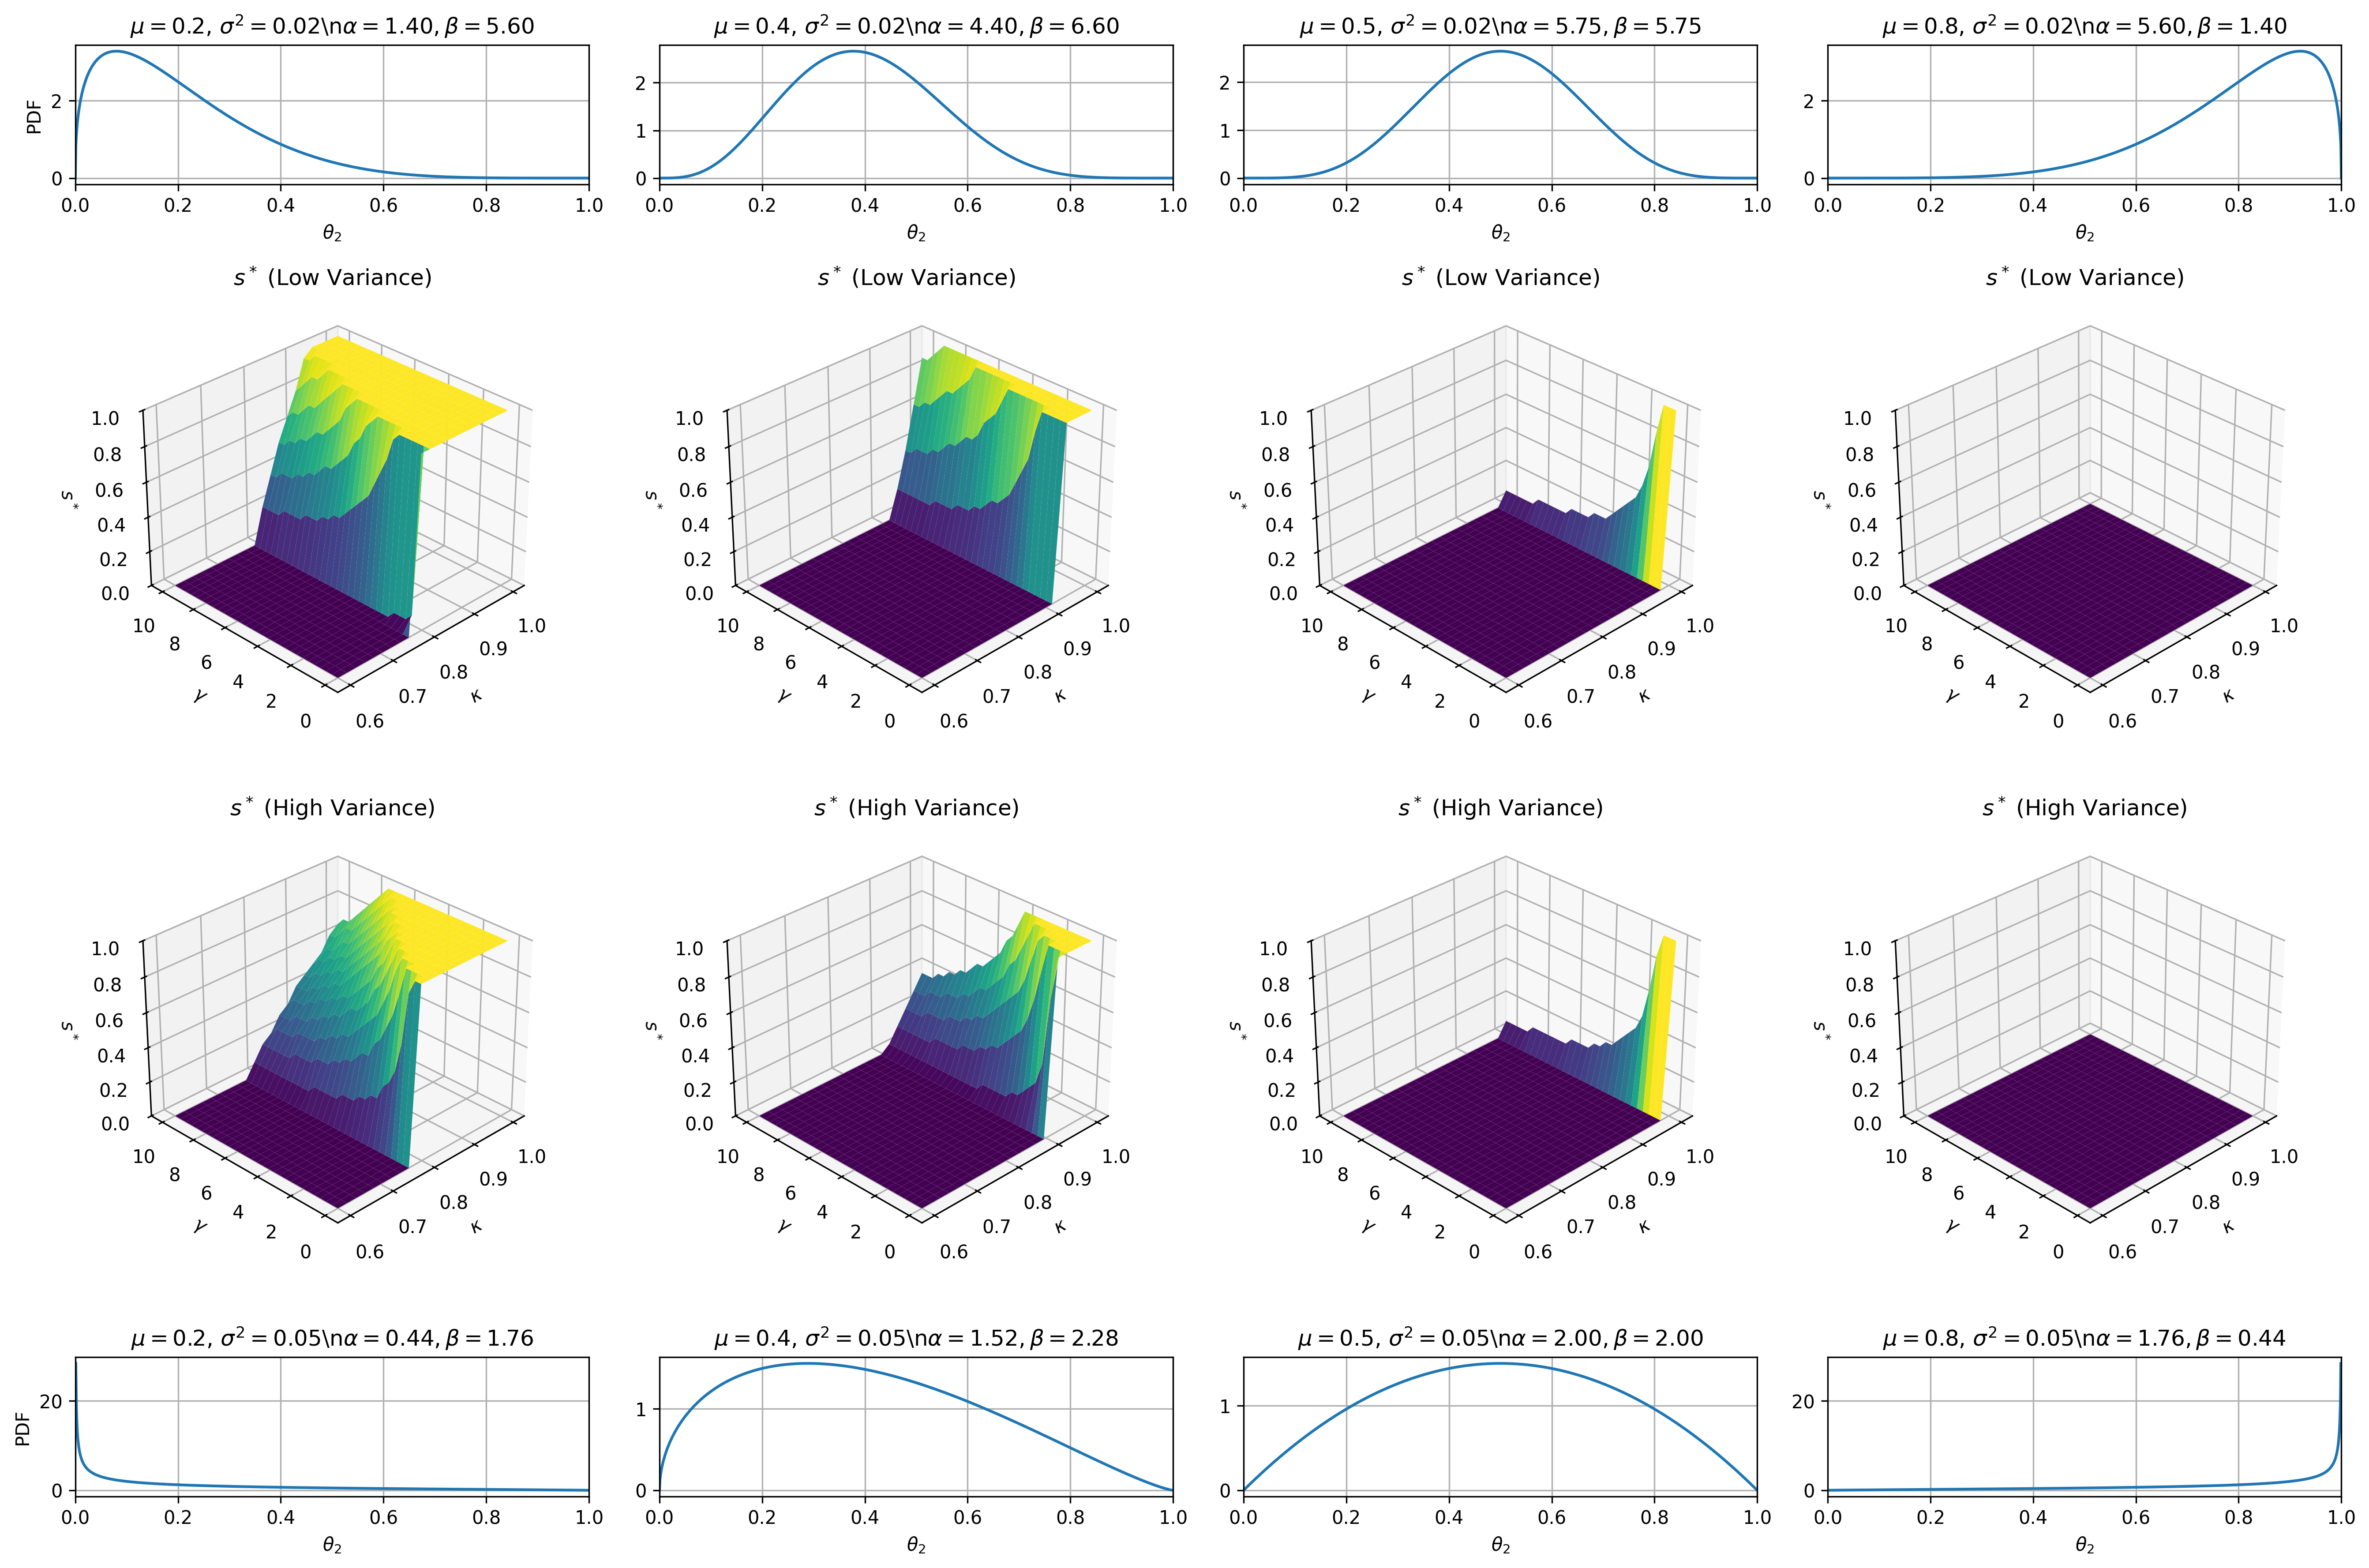
\includegraphics[width=\textwidth]{model_figures/3D_formulation.png}
\caption{Optimal Storage Share and PDF Visualizations under Eight Beta Distributions of $\theta_2$}
\label{Figure:3D_formulation}
\end{figure}

In general, when the farmer expects buyer power to be stronger in the future than at harvest-that is, when $\mathbb{E}[\theta_2] > \theta_1$-the incentive to store totally disappears. In other words, farmers would never store when $\mu > 0.5$ in our simulation here. As illustrated in the far-right column of the panel, the optimal strategy across all risk and efficiency levels is to sell immediately ($s^* = 0$).

Even when $\mathbb{E}[\theta_2] = \theta_1$, a farmer may still find storage worthwhile when he or she has a super high storage efficiency. This arises because the expected second-period price $\mathbb{E}[p_2] = \mathbb{E}\!\left[\frac{1}{1+\theta_2}\right]$ slightly exceeds the deterministic benchmark $\frac{1}{1+\mathbb{E}[\theta_2]} = p_1$, owing to the concavity of the price function in $\theta_2$. In other words, uncertainty in buyer power is beneficial from the farmer’s perspective: random fluctuations in $\theta_2$ generate an upward Jensen effect on expected prices. Consequently, even when the mean level of buyer power is unchanged across periods, the convexity of payoffs with respect to price risk induces modest positive storage in expectation.

In contrast, when expectations about future buyer power are favorable ($\mathbb{E}[\theta_2] < \theta_1$), the decision becomes more nuanced. Interior solutions ($0 < s^* < 1$) emerge over a meaningful range of risk preferences and storage efficiencies. Moreover, as the expected buyer power $\mathbb{E}[\theta_2]$ declines, both the scope for interior solutions and the frequency of corner solutions with full storage ($s^* = 1$) expand, reflecting the improved relative attractiveness of deferring sales.



Within each simulated surface, $s^*$ is non-increasing in $\gamma$. This pattern is especially pronounced when future buyer power is moderate-that is, when expected second-period prices are only marginally higher than those in the first period. The underlying mechanism is intuitive: risk-averse farmers increasingly value certainty over potentially higher but uncertain future payoffs. As $\gamma$ rises, the disutility associated with price risk begins to outweigh the intertemporal arbitrage opportunity, especially when those gains are compressed by relatively high buyer power.



In contrast, storage efficiency $\kappa$ plays a reinforcing role. For a given level of risk aversion, increases in $\kappa$ make storage more attractive by reducing the effective cost of waiting. Accordingly, $s^*$ is non-decreasing in $\kappa$. The responsiveness of $s^*$ to $\kappa$ weakens at higher values of $\gamma$, suggesting that even highly efficient storage systems cannot fully offset the behavioral costs of risk exposure when farmers are strongly averse to uncertainty. 


Cross-panel comparisons further illustrate how changes in the distribution of second-period buyer power affect storage incentives. As the mean future buyer power $\mu_{(\theta_2)}$ increases (moving left to right across the panels), expected second-period prices decline, rendering storage less attractive in expected-value terms. Accordingly, the optimal storage share $s^*$ shifts downward across the entire surface. This effect is especially pronounced for risk-neutral or mildly risk-averse farmers, who condition decisions almost exclusively on expected returns. The lower the expected future price, the more immediate sale becomes the dominant strategy.


Variance in buyer power exerts a subtler yet systematic influence. Comparing the second and third rows of the panel, low versus high variance cases, shows that greater dispersion in future buyer power ($\sigma^2$) consistently discourages storage, especially among the most risk-averse farmers. The mechanism is straightforward: higher variance increases downside risk in second-period returns, and with concave utility, this uncertainty weighs more heavily for those with stronger risk aversion. While highly risk-averse farmers are already reluctant to store, an increase in variance further reinforces their preference for immediate sale. By contrast, at low or moderate levels of $\gamma$, the marginal effect of variance is smaller, as these farmers are less sensitive to additional risk.



\subsection{Rarity of Interior Solutions}
Interior solutions, where the farmer chooses to allocate positive fractions of the harvest to both the first and second periods, are rare in this framework. The logic is straightforward: when the intertemporal trade-off is starkly tilted in favor of one period (either due to realization of $\theta_1$ relative to expected second-period buyer power $\mu$, extreme risk preferences, or inefficient storage), the farmer's best response is to sell all in one period. This is consistent with fieldwork evidence in the fresh apple industry in Central China: most apple growers tend to make corner decisions, either storing nearly everything when they expect future prices to be favorable, or selling everything immediately when uncertainty or storage cost dampens the incentive to wait. Within the model, such corner solutions arise from the nonlinearity of the CRRA utility function combined with the hyperbolic dependence of price on buyer power, which amplifies small differences in expectations or attitudes into decisive action.

To better understand the conditions under which interior solutions might arise, I extract a few representative cases from the simulation results shown in Figure~\ref{Figure:3D_formulation}. These examples are selected from scenarios with low variance in second-period buyer power and a low mean, specifically $\mu = 0.2$, where the distribution of future prices is skewed toward favorable outcomes. I restrict attention to moderate levels of risk aversion and relatively high storage efficiency, where neither risk nor cost fully dominates the farmer's decisions.

In the first case, I consider a farmer with a risk aversion coefficient of $\gamma = 2$ and a storage efficiency of $\kappa = 0.80$, with an expected second-period buyer power of $\mu = 0.2$. Here, this farmer's optimal choice is to store approximately 80\% of the harvest. The low expected buyer power implies a high expected price in the second period, while the relatively efficient storage technology ensures that much of this value is preserved. The farmer, though risk averse, finds it worthwhile to defer income but hedges by selling a small portion immediately. This behavior aligns well with farmers who have moderate patience and risk tolerance and access to good post-harvest storage infrastructure.

In the second case, I increase risk aversion to $\gamma = 2.75$, holding $\kappa = 0.80$ and $\mu = 0.2$ constant. The optimal storage share drops to about 62.5\%. The higher risk aversion amplifies the farmer's sensitivity to downside risk in second-period prices, even though the mean is favorable. The farmer still stores the majority, but the share sold in the first period increases, locking in a greater share of income from the crop. This behavior exemplifies more cautious farmers who hedge against worst-case outcomes even when market fundamentals appear strong.

In the third case, I keep risk aversion fixed at $\gamma = 2.75$ but reduce storage efficiency to $\kappa = 0.68$. The optimal storage share declines further to about 46\%. The decline in $\kappa$ reduces the effective return to deferred sales, making immediate selling relatively more attractive. This farmer, facing the same preferences and expectations as in the previous case, responds not to belief or attitude but to technical constraint. It reflects real-world circumstances where storage facilities are substandard or subject to losses from spoilage, pests, or theft-conditions that naturally discourage holding output even among patient, forward-looking producers.

Together, these three cases illustrate the sharp responsiveness of the storage decision to both preferences and storage costs. As risk aversion increases, storage declines, all else equal. And for a fixed level of risk aversion, lower storage efficiency can easily shift the farmer from a moderately storage-heavy strategy to one that leans toward immediate sale. Crucially, these interior solutions emerge only under a narrow configuration of parameters: relatively favorable and stable expectations, moderate caution, and at least tolerable storage conditions. Once any of these dimensions shifts toward uncertainty, risk aversion, or storage economic inefficiency, the solution quickly reverts to a corner.

In summary, interior solutions occur only when multiple forces---expected price gains, risk preferences, and storage efficiency---are delicately balanced. These cases are not typical but represent transitional zones in the farmer's decision space. Their rarity in both theory and field data affirms the robustness of the model's prediction: for most farmers, especially under poor storage conditions, decisive corner choices are the norm.




\subsection{Sensitivity: Expected Future Buyer Power and Risk Aversion}
\noindent To further examine how a farmer's optimal storage share $s^*$ responds to varying expectations about future buyer power, I conducted a simulation with the same parameter setting as in the 3D graphics above by holding first-period buyer power fixed at $\theta_1 = 0.5$, with a storage efficiency of $\kappa = 0.9$. The second-period buyer power $\theta_2$ was modeled as a Beta-distributed random variable with support on $[0, 1]$, maintaining a fixed variance of 0.02 while allowing the mean to vary from 0.05 to 0.95. For each mean value, I derived the associated Beta shape parameters and simulated 5,000 draws of $\theta_2$. The optimal storage share was then computed by maximizing expected utility under CRRA preferences, evaluated across five levels of risk aversion: $\gamma \in \{0, 0.5, 2, 4, 7\}$. As shown in Figure~\ref{Figure: sensitivity to second-period buyer power}, each resulting function $s^*(\mathbb{E}[\theta_2])$ was plotted to visualize how forward-looking uncertainty and risk preferences jointly shape storage behavior. Line color was varied monotonically with $\gamma$, increasing in darkness as risk aversion intensified.

The results reveal a distinct shift in behavior across risk preference levels. Under risk neutrality ($\gamma = 0$), the decision rule is binary: the farmer stores all output if the expected net-storage-cost second-period price exceeds the current one, and none otherwise. As $\gamma$ increases to positive values, the decision becomes more nuanced. The sharp threshold gradually turns into a smooth, decreasing function of $\mathbb{E}[\theta_2]$, with interior solutions appearing when the expected future buyer power is only marginally lower than the first-period one.


With higher risk aversion (like $\gamma = 4$ and $\gamma = 7$), the willingness to store declines substantially. Even when the expected second-period price exceeds today's price, the farmer often chooses to sell immediately due to the downside risk embedded in the distribution of $\theta_2$. The curve $s^*(\mathbb{E}[\theta_2])$ flattens near zero, and the turning point at which storage becomes attractive shifts leftward. This leftward shift reflects a heightened preference for certainty: more favorable expectations are required before any intertemporal transfer of output becomes worthwhile. 


\begin{figure}[ht!]
\centering
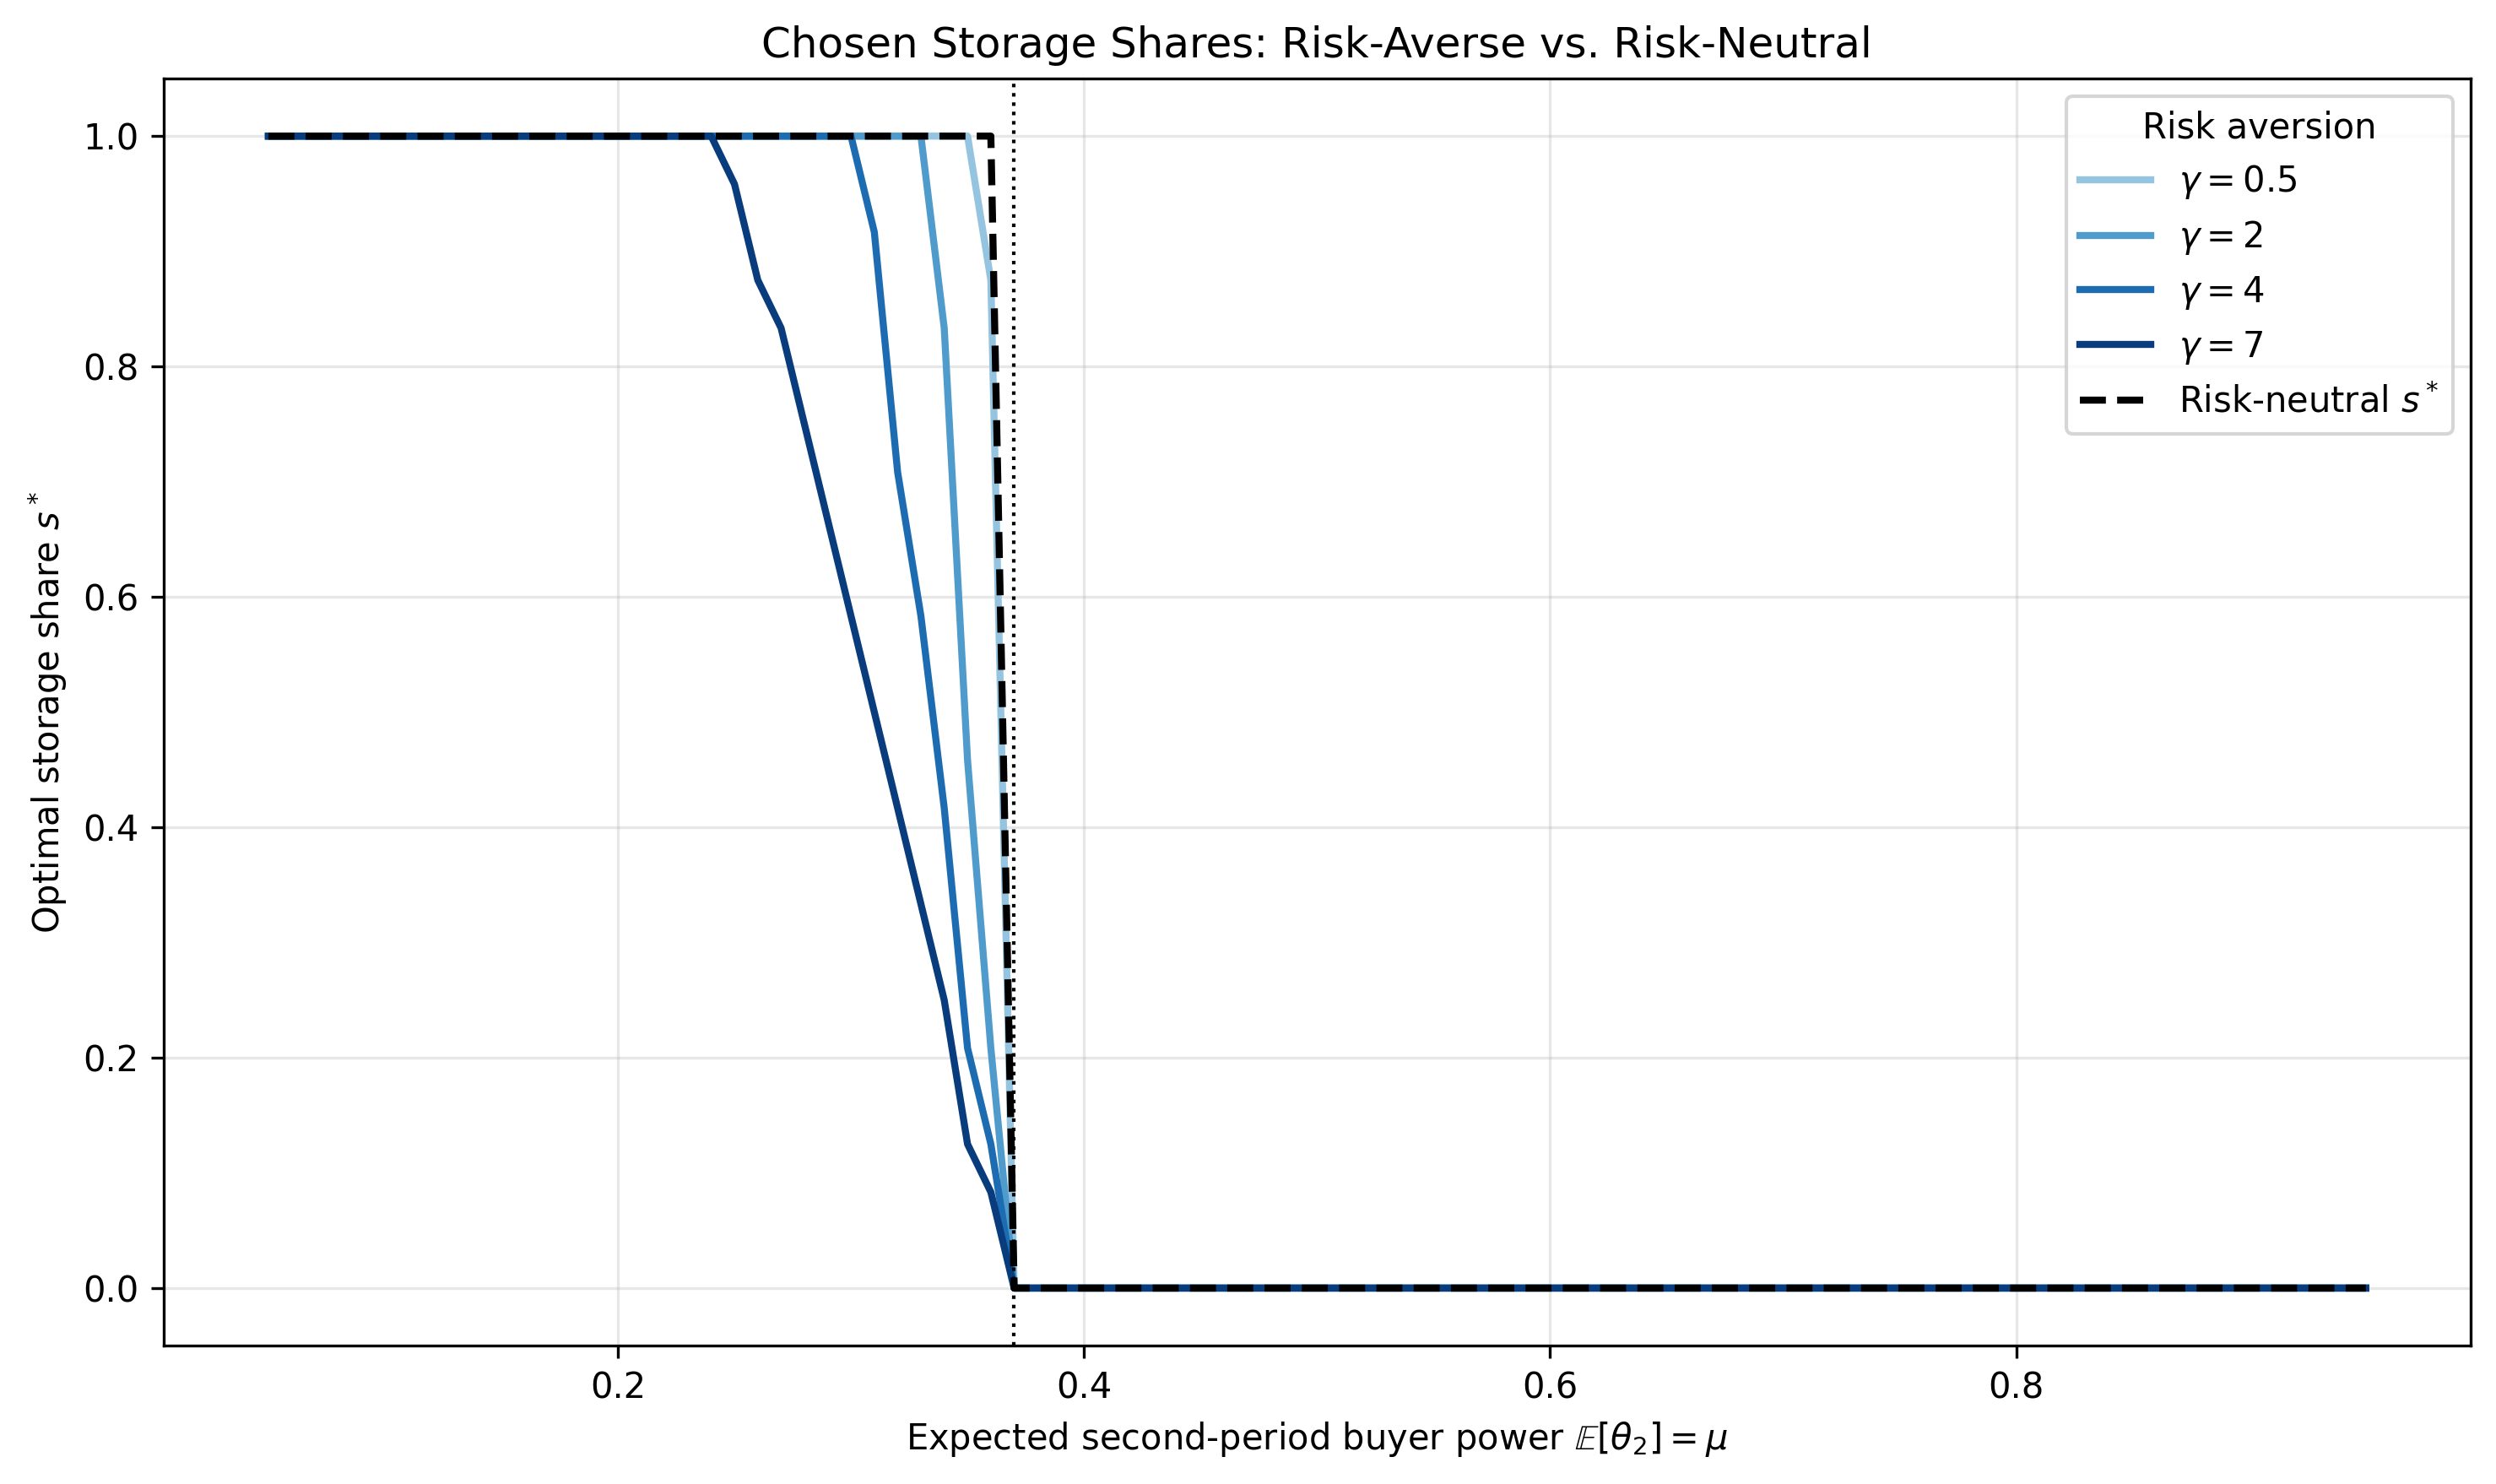
\includegraphics[width=\textwidth]{model_figures/sensitivity_to_theta_2.png}
\caption{Sensitivity to Expected Second-Period Buyer Power}
\label{Figure: sensitivity to second-period buyer power}
\end{figure}

\begin{figure}[ht!]
\centering
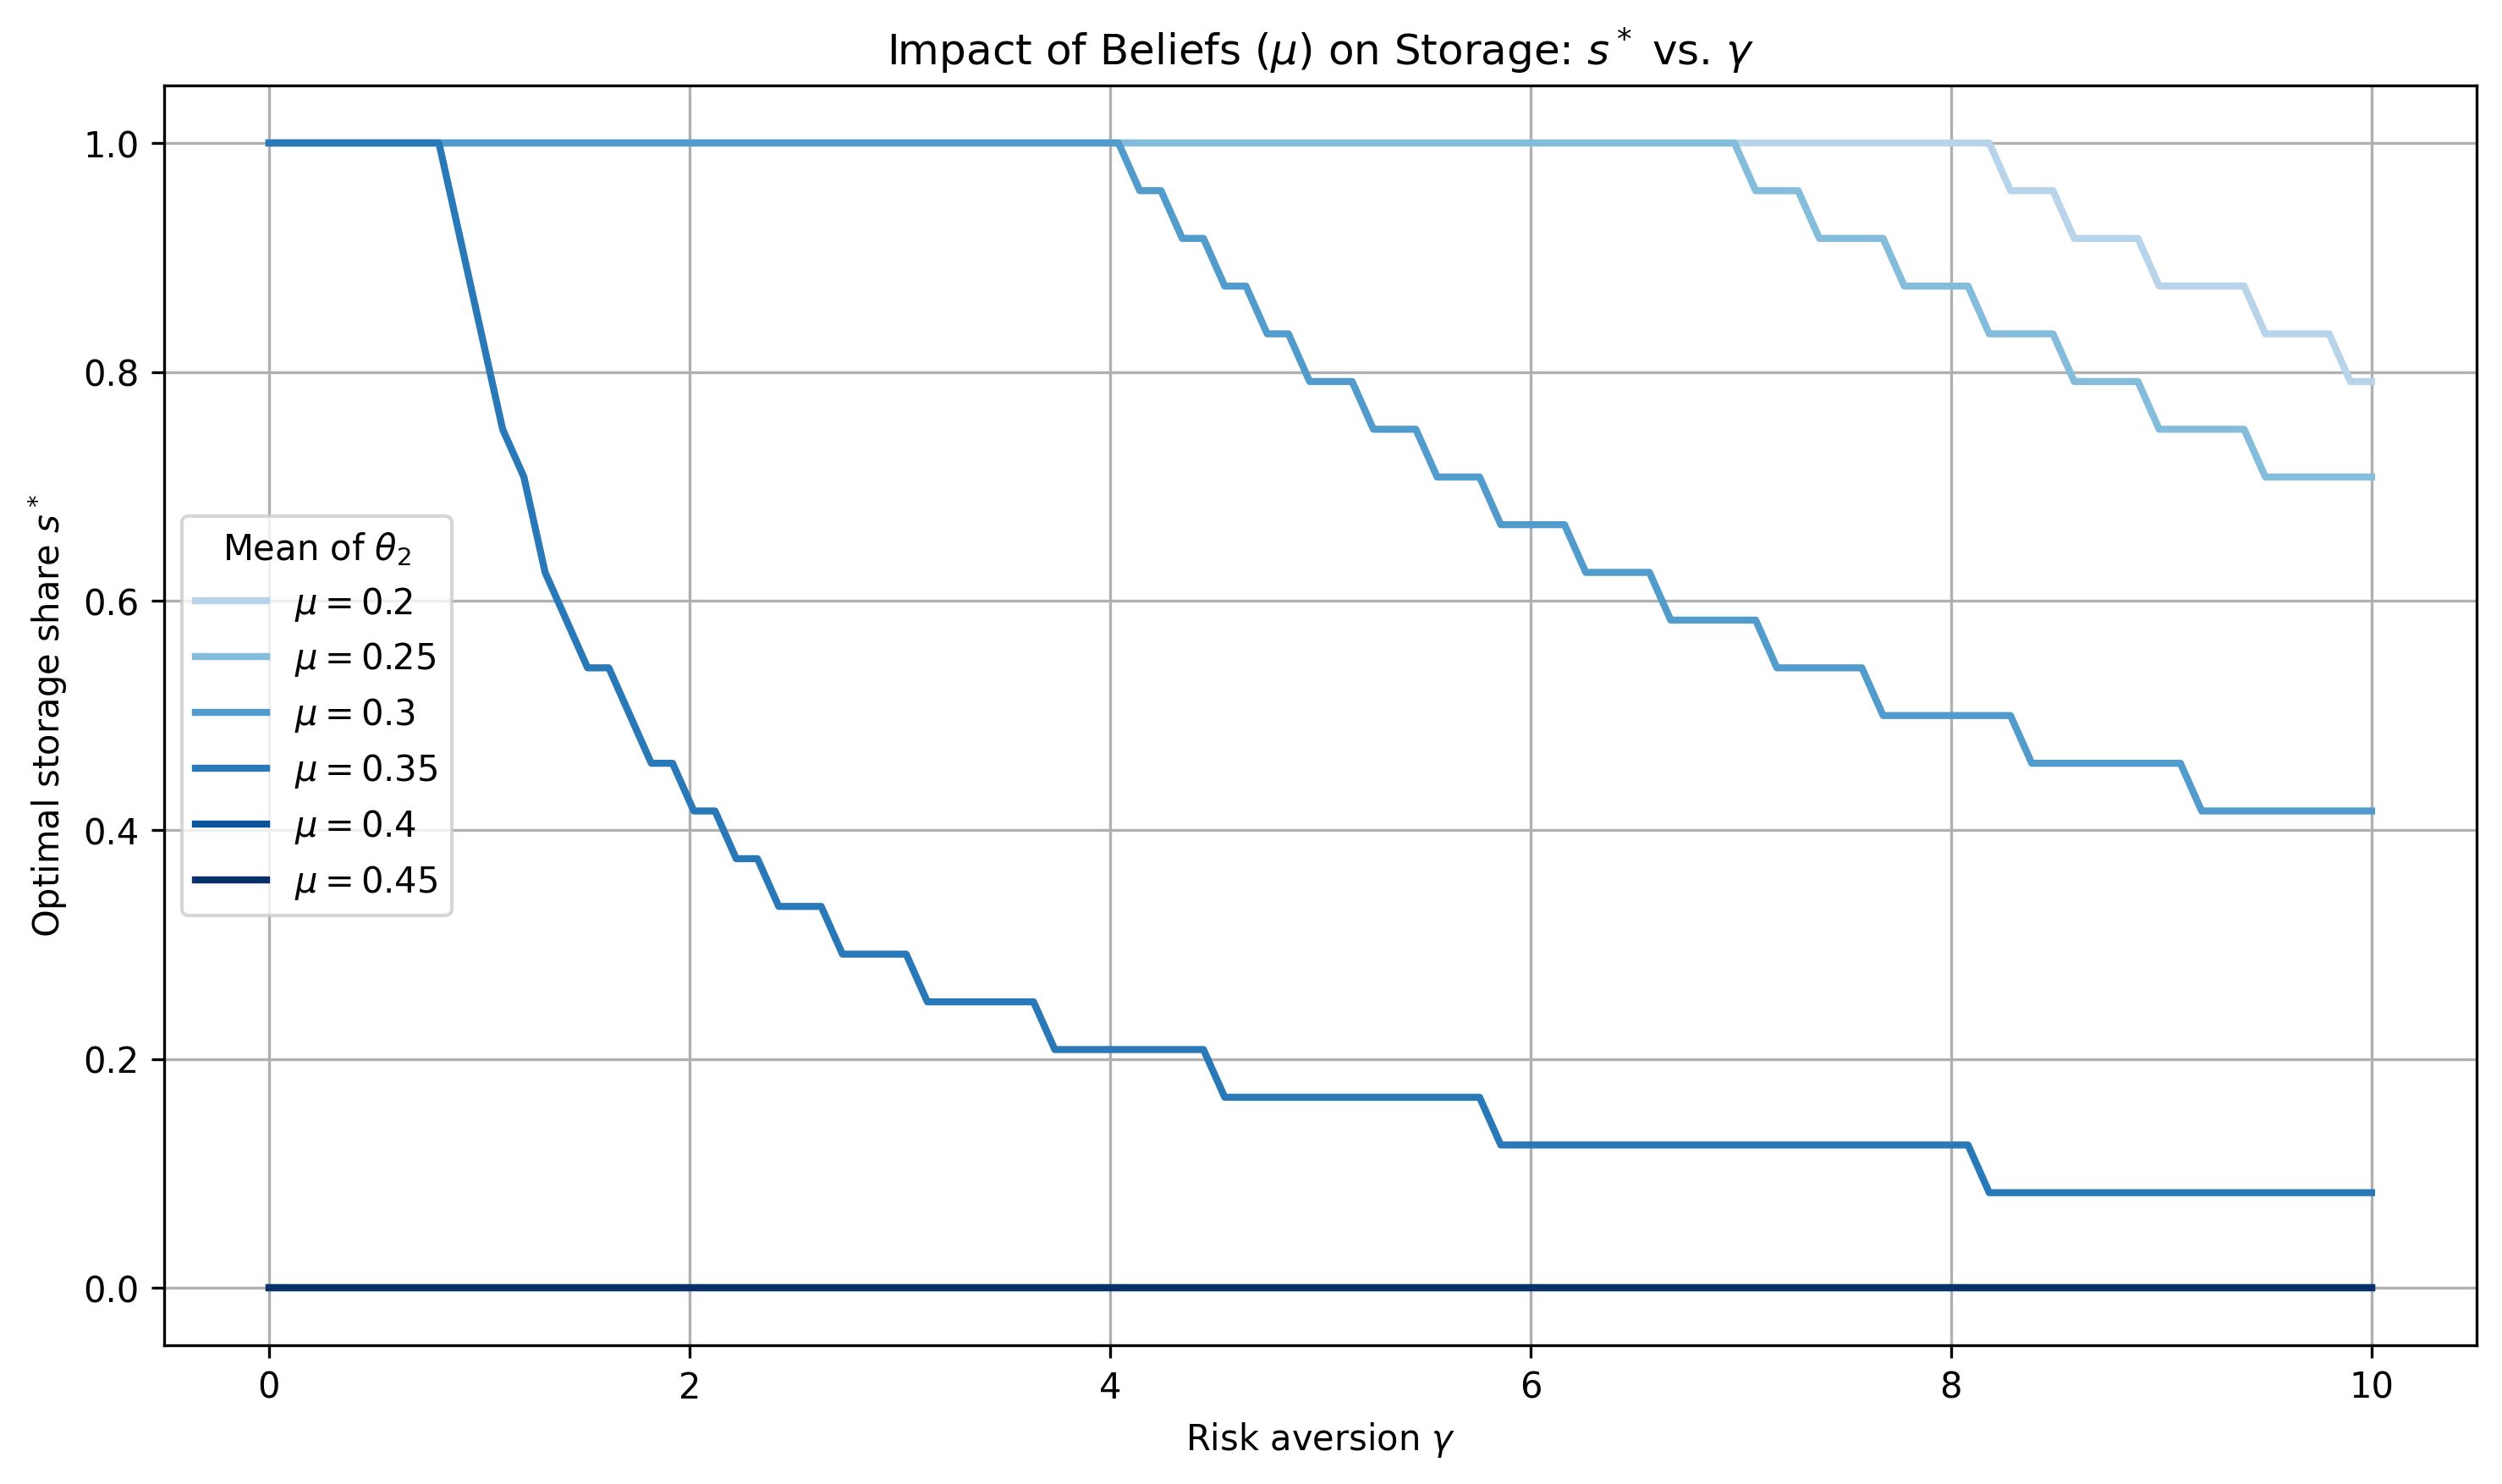
\includegraphics[width=\textwidth]{model_figures/sensitivity_to_gamma.png}
\caption{Sensitivity to Risk Aversion}
\label{Figure: sensitivity to risk aversion}
\end{figure}


In addition, I constructed another visualization in Figure~\ref{Figure: sensitivity to risk aversion} that examines how a farmer's optimal storage share responds to changes in risk aversion, under varying expectations about future buyer power. With the same parameter setting as in the 3D graphics above, I simulate buyer power beliefs using Beta distributions with means ranging from $\mu = 0.2$ to $\mu = 0.4$ in increments of 0.05. For each mean, I compute the corresponding shape parameters $(\alpha, \beta)$, draw 5,000 samples of $\theta_2$, and evaluate the expected utility under a CRRA utility function across 100 grid points of $\gamma \in [0, 10]$. The optimal storage share $s^*$ is computed by maximizing the expected utility over a grid of candidate values $s \in [0, 1]$, reflecting the proportion of harvest stored for second-period sale. Also, Figure~\ref{fig:unified_gap_plot}, discussed later in policy implications, quantifies the income consequences of risk aversion, showing both the absolute and proportional losses relative to the risk-neutral benchmark across the range of expected buyer power.



The resulting graph in Figure~\ref{Figure: sensitivity to risk aversion} plots $s^*$ against $\gamma$ for each value of $\mu$. Several patterns emerge clearly. First, storage shares generally decline with increasing risk aversion, but the relationship is not strictly monotonic. Over some ranges of $\gamma$, the curves flatten, indicating regions where changes in risk aversion have little effect on storage behavior. In these cases, either the expected price advantage or the storage cost dominates the decision, making farmers' optimal storage choices relatively insensitive to marginal changes in risk preferences. 

Second, higher expected buyer power in the second period (i.e., higher $\mu$) uniformly depresses the storage share. When future market power is expected to be strong (i.e., lower $p_2$), forward sales become less attractive, reinforcing the incentive to sell early regardless of risk preferences.

Interestingly, the sensitivity of $s^*$ to risk aversion ($\gamma$) becomes more pronounced as the expected future buyer power ($\mu$) approaches the current level $\theta_1$. When $\mu$ is low (e.g., $0.2$), storage remains attractive even for highly risk-averse farmers, as the expected second-period price is sufficiently high to compensate for risk. As $\mu$ increases (e.g., to $0.35$), the storage share declines sharply at relatively low levels of $\gamma$, indicating that even moderately risk-averse farmers prefer to sell immediately when future price expectations weaken. Consistent with Figure~\ref{Figure: sensitivity to second-period buyer power}, when $\mu = 0.4$, no farmer stores at all, since the expected price advantage is fully eroded by the effective storage costs.


This graphical structure complements prior results showing $s^*$ as a function of $\mu$ at fixed $\gamma$. Together, they offer a two-dimensional understanding of farmer behavior: beliefs about future buyer power shift the entire $s^*(\gamma)$ curve, while changes in risk aversion tilt its shape. These patterns are particularly relevant for understanding heterogeneous storage behavior across farmers who face similar market fundamentals but differ in attitudes toward risk or expectations about downstream market structure.



\section{Policy Implications}
\noindent
Whether in developing or advanced economies, policymakers care deeply about farm incomes. A common response has been direct interventions, such as minimum support prices or income transfers, that boost incomes but often at the cost of market distortions, fiscal burden, and misallocation of resources. The model here suggests an alternative emphasis: improve the environment in which farmers make intertemporal selling decisions. Three margins emerge from the analysis, competition, storage efficiency, and risk aversion, each capable of lifting expected incomes without direct price manipulation.



\subsection{Enhancing Competition among Buyers}

\textbf{Mechanism.} When competition among buyers is weak at harvest, farmers face low farm-gate prices. In the model this is captured by a high $\theta_1$, which depresses the immediate return to selling. Storage provides farmers with the option value of waiting, and its payoff rises if competition is expected to be stronger in the future, i.e.\ when the mean of $\theta_2$ falls and the second-period price distribution shifts upward. In this way, stronger future competition amplifies the benefits of storage by improving the relative return to waiting rather than selling at harvest.

\textbf{Quantitative illustration ($\kappa=0.9$, $\text{Var}(\theta_2)=0.02$):}
\begin{itemize}
  \item Suppose $\theta_1=0.5$ (harvest price $p_1=0.667$) and beliefs about buyer power shift from $\mu=0.37$ (weaker future competition) to $\mu=0.32$ (stronger future competition). Risk-neutral and risk-averse ($\gamma=2$) farmers both switch from \emph{no storage} to \emph{full storage}. Expected income rises from $0.667$ to $0.690$, a gain of $+\;0.023$.
\end{itemize}

\textbf{Policy interpretation.} When policies succeed in enhancing buyer competition at harvest, the immediate farm-gate price $p_1$ rises, thereby improving farmer welfare unconditionally. In practice, however, such interventions may not always produce an immediate effect at the start of the marketing season. The model indicates that as long as buyer competition improves at any point during the marketing period, farmers can still possibly benefit through storage. Relevant policy instruments include stricter antitrust enforcement to deter collusion, lowering entry barriers for new traders, and investments in digital trading platforms or logistics infrastructure that expand farmers' access to alternative buyers throughout the season.






\subsection{Improving Storage Efficiency} \label{sec:storage-efficiency}

\textbf{Mechanism.} 
An increase in storage efficiency, represented by a higher $\kappa$, raises the expected return from delaying sales. Farmers effectively preserve a larger share of the crop’s value, making intertemporal arbitrage more attractive. The effect is strongest when market conditions are expected to be better: even a modest gain in $\kappa$ can induce a shift from immediate sale to full storage. 

The welfare implications, however, depend on which producers adjust behavior. For farmers who would have stored fully regardless, a higher $\kappa$ merely transfers income. The principal welfare gains arise among marginal storers, those who switch from zero to positive storage or from partial to full storage. Only for these producers does the policy alter real storage decisions.


\textbf{Quantitative Illustration.} 
Consider a policy intervention that raises $\kappa$ by 10\%. Let $\operatorname{var}(\theta_2)=0.02$ and examine risk aversion at $\gamma \in \{0,\,0.5,\,2,\,4\}$. Figure~\ref{fig:storage_kappa} reports the induced changes in expected income, $\Delta E[\pi]$, and optimal storage share, $\Delta s^*$.

\emph{Symmetric buyer power ($\theta_1 = E[\theta_2]$).} 
Under symmetric expectations, storage efficiency improvements have subtle impacts on a farmer's welfare. When initial efficiency is $\kappa_0 = 0.70$ or $0.80$, the $\Delta E[\pi]$ curves are essentially zero across all $\mu$, indicating negligible behavioral response. At $\kappa_0 = 0.90$, however, $\Delta E[\pi]$ becomes positive and declines with $\mu$: farmers facing lower mean buyer power (low $\mu$) experience greater gains because higher $\kappa$ triggers a shift from no to positive storage. Random variation in $\theta_2$ generates a Jensen effect on expected second-period prices, confirmed by a modest upward movement in the $\Delta s^*$ panel. These effects are much smaller than in the asymmetric case below.


\emph{Fixed current buyer power ($\theta_1 = 0.5$).} 
When current buyer power is fixed at $0.5$, both the level and shape of the curves change. In the $\Delta E[\pi]$--$\mu$ panels, all $\kappa_0$ lines start high at low $\mu$ and converge toward zero as $\mu$ rises. These higher curves, relative to the symmetric case above, reflect the larger value of delaying sales when the current price is weak. 

The $\Delta s^*$ panels exhibit a clear pattern. For $\kappa_0 = 0.70$, farmers transition from no to partial storage within a narrow $\mu$ interval---a steep ``hill.'' As $\kappa_0$ rises to $0.80$ and $0.90$, the hill shifts rightward, indicating that more farmers are already full storers and the pool of potential switchers narrows. 

Consequently, a 10\% improvement in $\kappa$ yields positive expected-income gains over a broader range of $\mu$ as baseline efficiency rises, but the behavioral margin drifts rightward.


\textbf{Policy Interpretation.} 
The simulations suggest that gains from improved storage efficiency are largest when future buyer power is expected to be weaker than current levels. As baseline efficiency increases, welfare effects become increasingly infra-marginal, and the $\Delta s^*$ ``hill'' in Figure~\ref{fig:storage_kappa} shifts rightward. 

Importantly, higher effective $\kappa$ need not result from direct subsidies to storage. Similar outcomes can arise if farmers discount future income less. For instance, through income safety nets that smooth consumption or credit access that relaxes liquidity constraints. Such mechanisms enhance intertemporal storage efficiency without direct fiscal expenditure.







\subsection{Reducing Effective Risk Aversion}

\textbf{Mechanism.} While intrinsic risk preferences are relatively stable, \emph{effective} risk aversion declines as farmers gain financial security through liquidity, insurance, and wealth accumulation. A lower coefficient of relative risk aversion ($\gamma$) shifts behavior toward the risk-neutral benchmark, with the largest effects concentrated in the region where storage is only marginally profitable in expectation.


\begin{figure}[ht!]
    \centering
    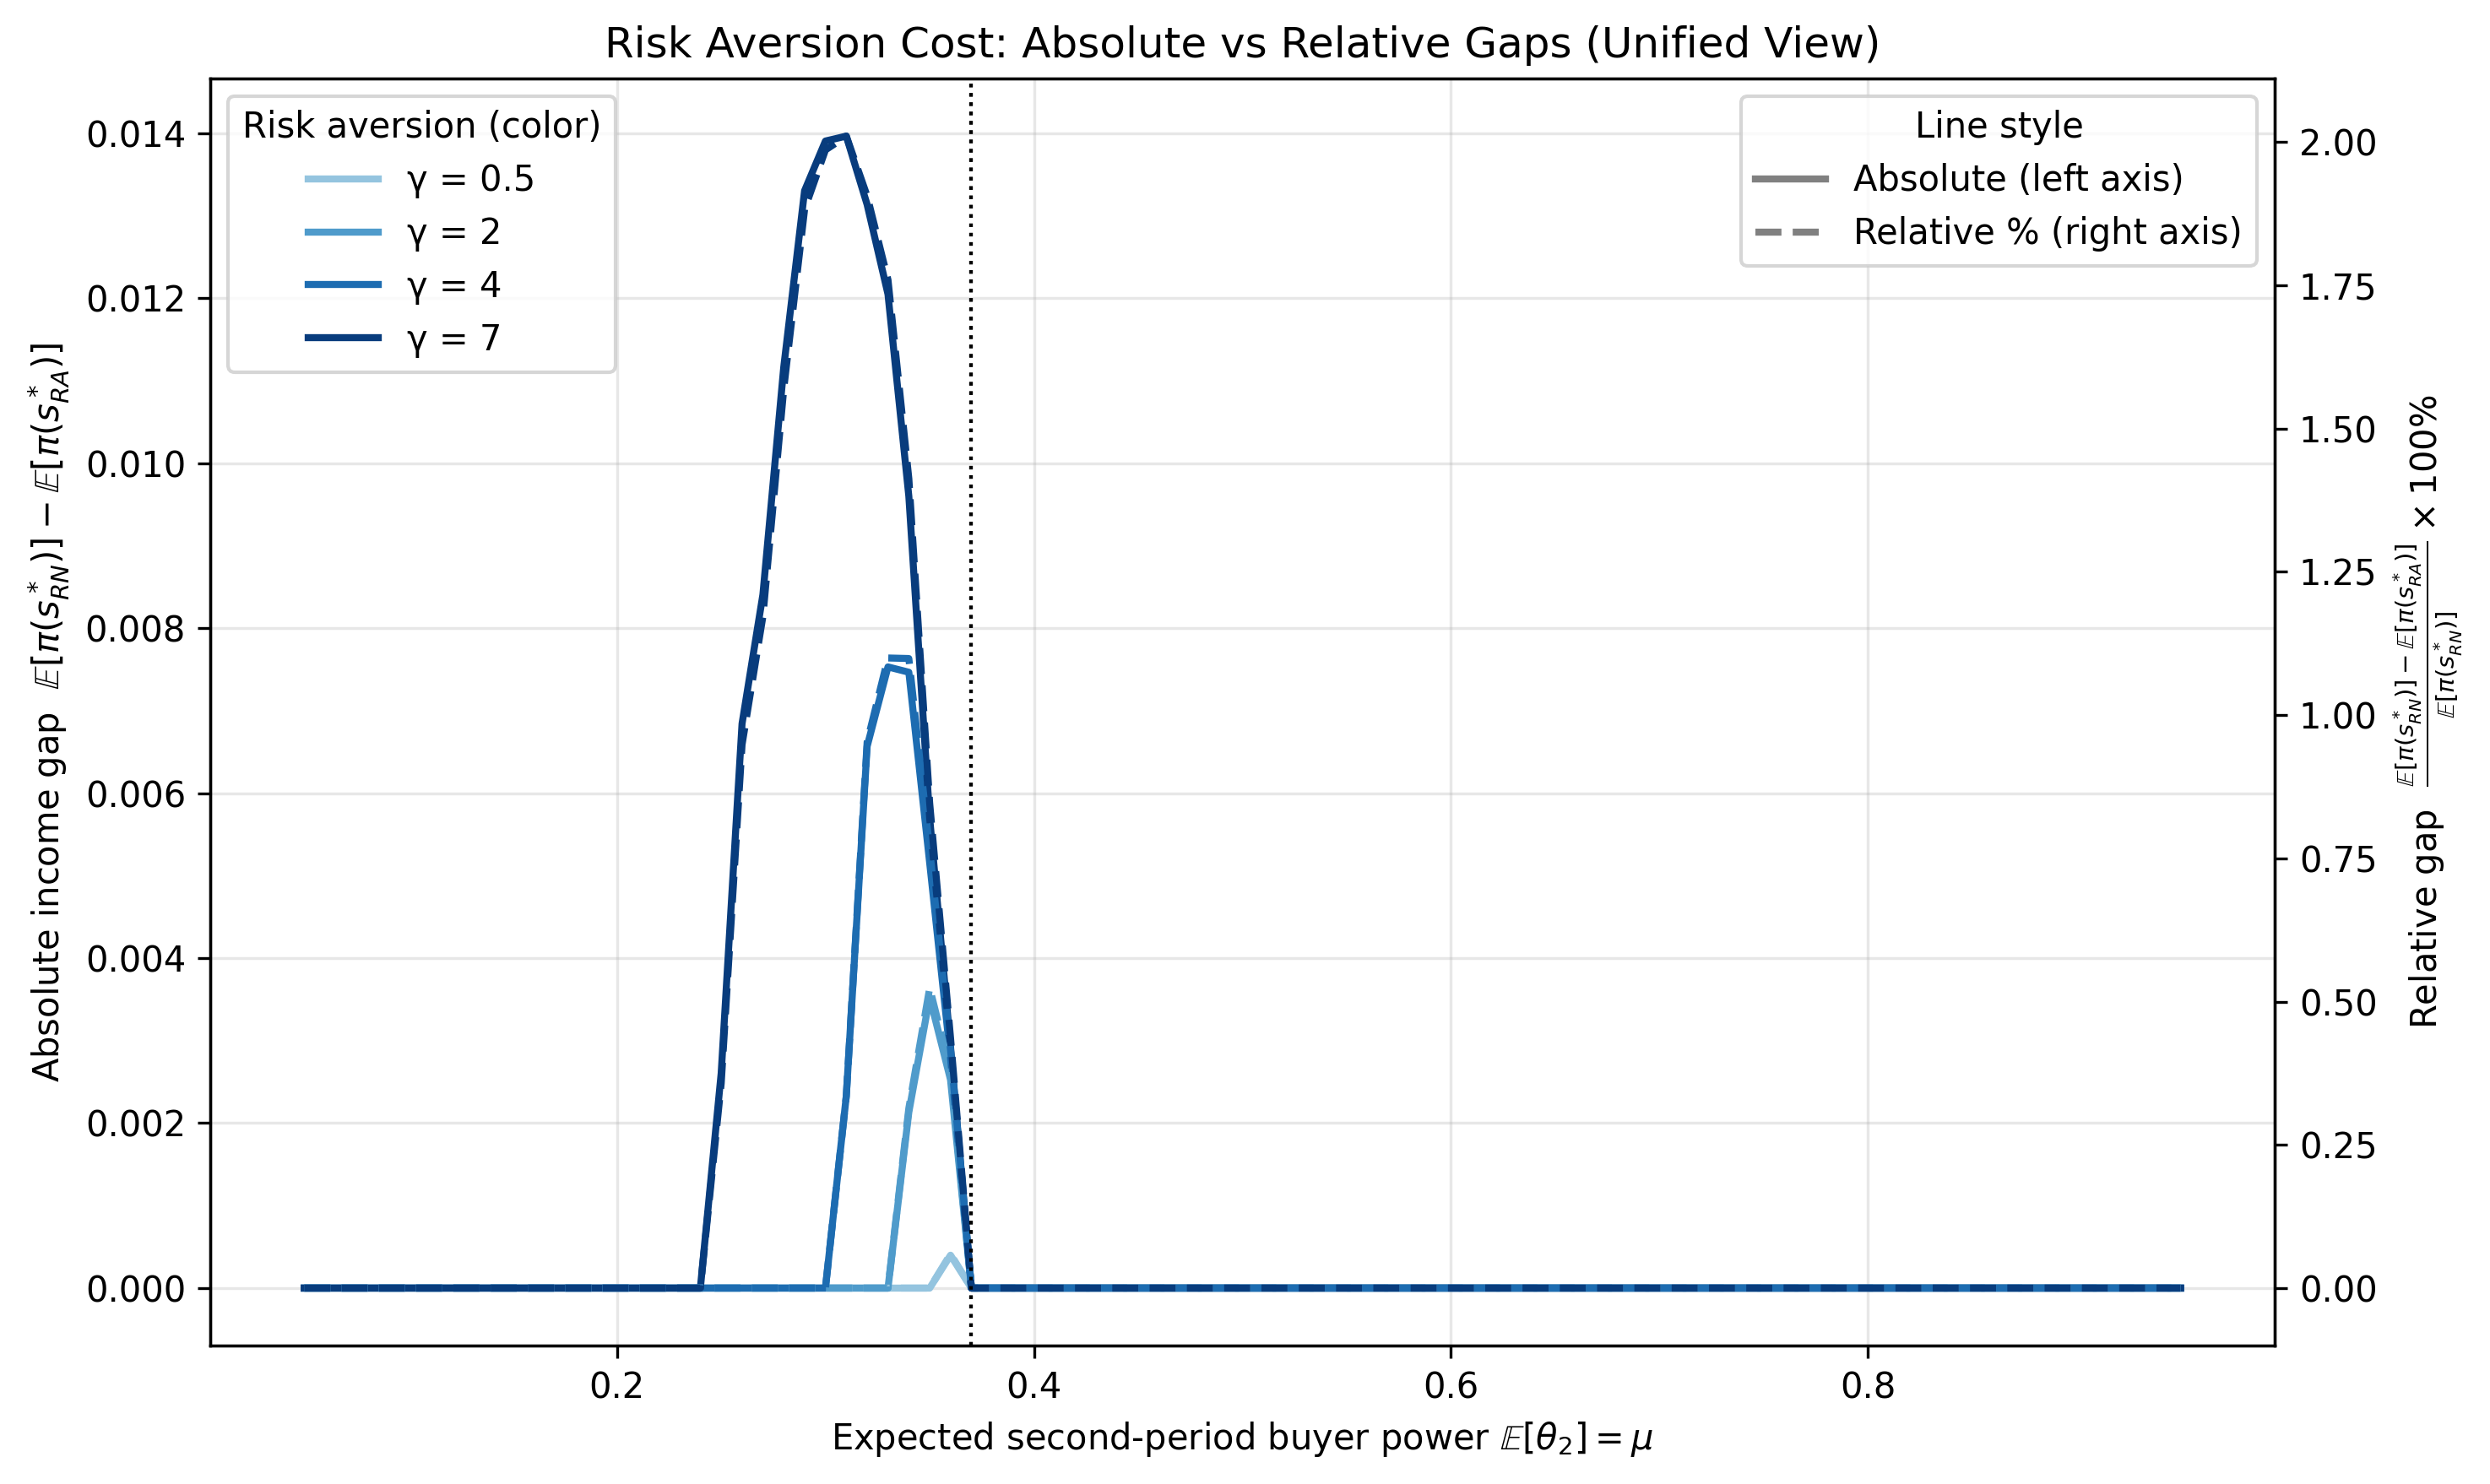
\includegraphics[width=0.85\textwidth]{model_figures/income_gap_vs_mu_(unified).png}
    \caption{Absolute and Relative Expected Income Losses from Risk Aversion}
    \label{fig:unified_gap_plot}
    \begin{tablenotes}
    \footnotesize
    \item Note: solid lines show the absolute gap $\mathbb{E}[\pi(s^*_{RN})]-\mathbb{E}[\pi(s^*_{RA})]$ (left axis). 
    Dashed lines show the same gap as a percentage of the risk-neutral benchmark (right axis). 
    Colors indicate the degree of risk aversion ($\gamma$). 
    The vertical dotted line marks the risk-neutral switching threshold $\mu^\star$ where storage ceases to be profitable.
    \end{tablenotes}
\end{figure}


\textbf{Quantitative illustration:} The Simulation results from the baseline model in Figure~\ref{fig:unified_gap_plot} show that absolute income losses from risk aversion peak at roughly 0.02--0.03 in normalized units, while the relative gap reaches about 2 percent of expected income under strong risk aversion ($\gamma=7$) and falls below 1 percent for moderate values ($\gamma=2$ to $4$). These effects vanish when storage is clearly profitable or clearly unprofitable, underscoring that the ``cost of risk aversion'' is concentrated exactly at the margin where storage incentives are fragile.

\textbf{Policy Interpretation.} The income effect from lowering risk aversion is modest in size but targeted: it recovers the ``money left on the table'' precisely where risk aversion binds most. Instruments that ease liquidity risk (warehouse-receipt finance, seasonal credit lines), transfer income across states (crop insurance), or smooth consumption (safety nets) can move farmers measurably closer to the risk-neutral storage decision. Even modest financial deepening---for example, reducing effective $\gamma$ from 7 to 2---eliminates more than half of the small but systematic income gap in this calibration.















\section{Special Cases: Explicit Competition Forms}\label{Section: Special Cases: Explicit Competition Forms}
\noindent In the base framework, buyer power was represented in a reduced-form manner typical of \textit{FOOM} models, where buyer power $\theta$ was treated as a latent, abstract variable inferred from observed farm-gate prices through a nonlinear transformation. Conceptually, $\theta$ can be thought of as a sufficient statistic for market structure and conduct: at one extreme, it may correspond to the number of downstream buyers $N$ (with higher $N$ implying weaker buyer power), while more generally it can capture the distribution of buyer market shares as well as the intensity of competition. For example, a low $\theta$ could reflect either many symmetric buyers competing aggressively, or a few large buyers that nonetheless compete rather than collude; conversely, a high $\theta$ could arise from concentrated market shares, tacit collusion, or explicit coordination. 

To move beyond this abstraction, I now introduce explicit models of non-cooperative buyer competition---namely, Bertrand (price-setting) and symmetric-buyer Cournot (quantity-setting) frameworks---thus ignoring for this analysis possible buyer collusion. These models provide structural microfoundations for $\theta$ by linking it to primitive features of market structure and strategic interaction.


Suppose farmers observe the number of buyers present in the village at harvest time in the first period, denoted by $N_1$, and form expectations about buyer presence in the second period, $\mathbb{E}[N_2]$. The number of buyers in each period is a discrete variable bounded between zero and a finite upper limit.

Bertrand and Cournot models offer contrasting benchmarks for non-cooperative buyer behavior. In the classic Bertrand setting, even a small number of buyers (as few as two) can generate highly competitive outcomes, a result often referred to as the ``Bertrand paradox.'' Translated into the present framework of traders purchasing from farmers, this implies that competition among a small set of buyers is sufficient to bid up the farm-gate price to the competitive benchmark---namely, the crop's \textbf{net marginal value product}, which by normalization equals 1.0 in the base model. In contrast, under Cournot competition the relationship between the number of buyers $N$ and the equilibrium farm-gate price is more gradual: as $N$ increases, buyer market power declines smoothly, and the farm-gate price converges to the competitive benchmark only asymptotically as $N \to \infty$.


To ground the discussion, I draw on my fieldwork among apple growers in Yanchang County, Central China, during the 2024-2025 agricultural year. According to my survey of the targeted 15 buyers, including the top five most influential local traders, the number of buyers visiting a village at harvest ranges from zero in remote areas to a maximum of nine.\footnote{In Figure~\ref{Figure: buyer count at harvest}, 26\% of farmers appear to forecast fewer than zero buyers in the future, which is clearly nonsensical. This artifact arises because my sample of 15 buyers does not exhaustively cover the entire population of potential buyers, only the majority of the most frequently observed ones. Hence, farmers expressing highly pessimistic expectations experienced buyer visits from buyers outside my sample.} The mean first-period buyer count is 3.34, with a median of 3. As shown in Figure~\ref{Figure: buyer count at harvest}, fewer than 7\% of surveyed growers reported no buyer presence during harvest (for simplicity, the Bertrand analysis excludes this case), while over 80\% experienced at least two buyer visits. Most farmers reported between two and five buyers, motivating my assumption of a Poisson distribution for second-period buyer counts in the Cournot analysis.

Importantly, farmers' expectations about second-period buyer presence appear weakly correlated with observed first-period buyer counts. This is illustrated by the color segments within each bar in Figure~\ref{Figure: buyer count at harvest}, which show considerable heterogeneity in forward-looking beliefs conditional on current buyer exposure.

\begin{figure}[ht!]
\centering
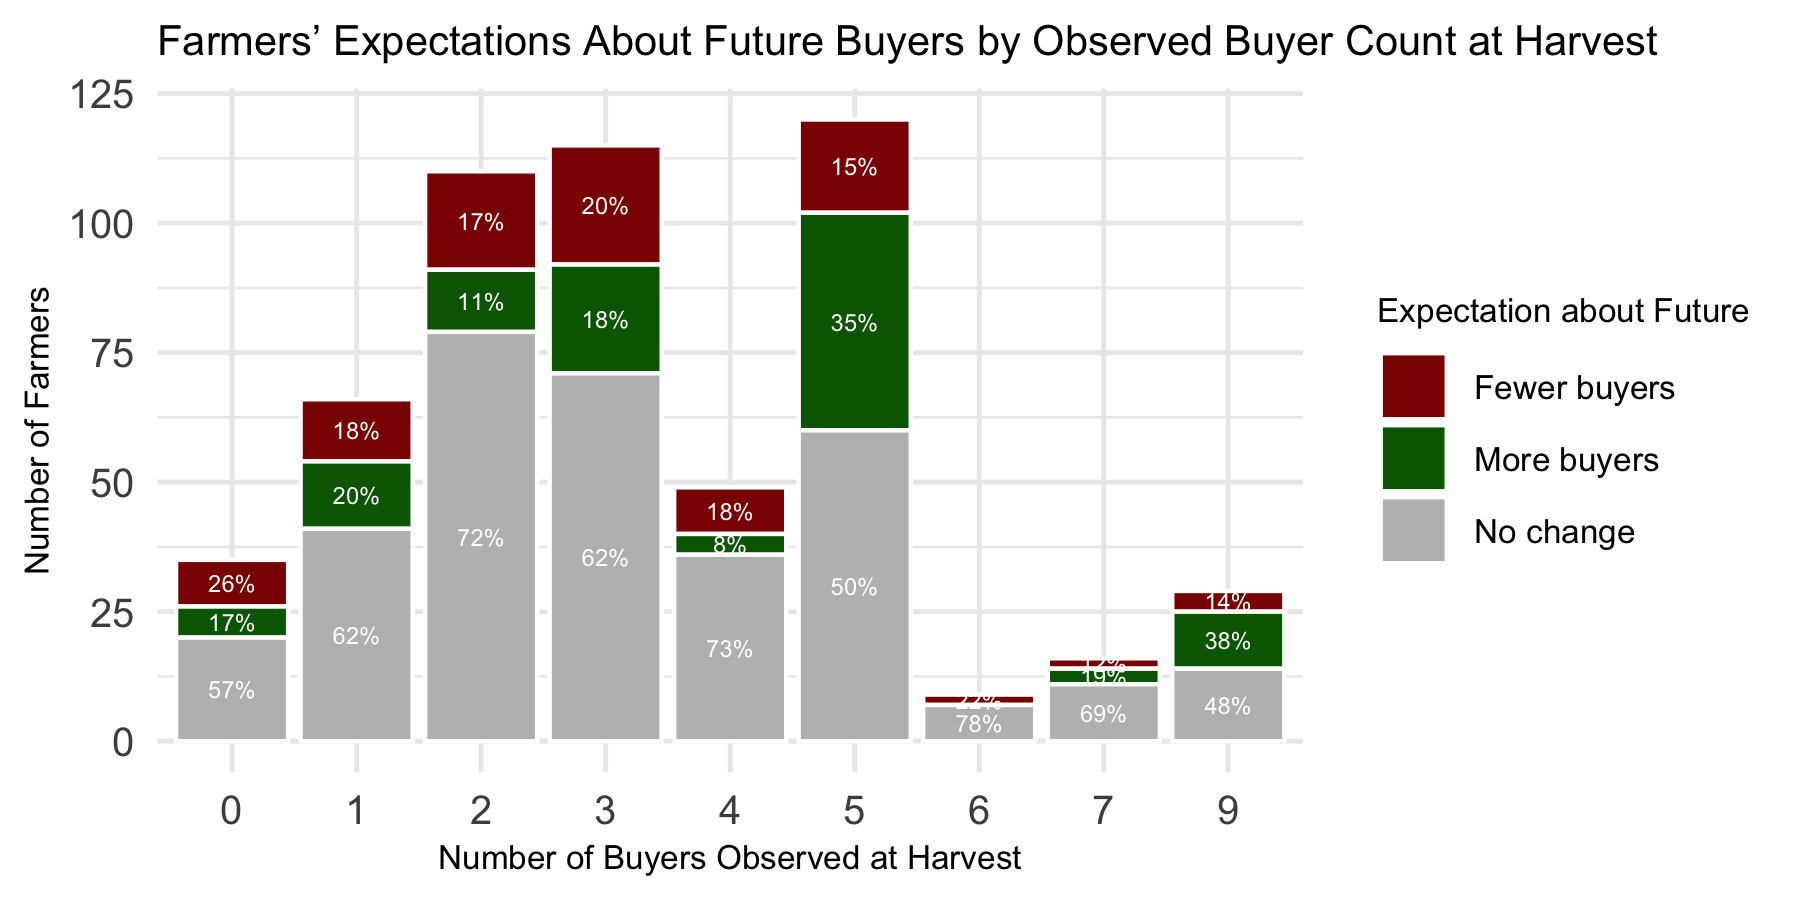
\includegraphics[width=\textwidth]{figures/buyer_count_distribution.png}
\caption{Observed Buyer Count at Harvest with Farmers' Expectations About Future Buyers}
\label{Figure: buyer count at harvest}
\end{figure}


\subsection{Price-Setting Competition: Bertrand--Nash Equilibrium}
\noindent In the price-setting environment, buyers set the price they offer to farmers. If there are no capacity constraints, the standard Bertrand logic applies: even two buyers suffice to drive the purchase price up to the competitive benchmark, which is normalized to 1 under our derived price formation rule in Equation~\ref{Eq: price formation by buyer power}. This outcome, often referred to as the Bertrand Paradox, corresponds here to a Bertrand--Nash equilibrium in which perfectly competitive outcomes ($\theta_t=0$) arise as long as $N_t \geq 2$.

Therefore, under Bertrand conditions, according to Equation~\ref{Eq: price formation by buyer power}, the farm-gate price received by farmers can be modeled as:
\begin{equation}
p_t = 
\begin{cases}
0.5, & N_t = 1 \\
1, & N_t \geq 2
\end{cases}
\label{Eq: Bertrand Price Schedule}
\end{equation}
\noindent where $0.5$ denotes the monopsonistic price paid when only one buyer is present. The transition from a single-buyer market to a multi-buyer market results in a discontinuous shift in price.

Here, I assume that farmers observe the first-period price at harvest, and the number of traders at a specific village in the second trading period ($N_2$) is stochastic, with the probability of one middleman being $\rho$, i.e., $Pr(n_2=1)=\rho$. So, the probability of multiple intermediaries appearing in village $j$ is $Pr(n_2 \geq 2) = 1-\rho$.

Therefore, a farmer's optimization problem in Equation~\ref{eq:final objective} could be written as follows:
\begin{equation}
\max_{s \in [0,1]} \psi(\cdot) = \rho U((1-s)p_1 + \kappa s \cdot 0.5) + (1-\rho) U \left( (1-s)p_1 +  \kappa s \cdot 1 \right)
\end{equation}
where the first expression on the right-hand side reflects the utility from storing $s$ share of production to the second period in the monopsonistic case, and the second term represents the utility in the case of perfect competition among buyers. 

Since all farmers would sell immediately at harvest when multiple buyers are present ($p_1 = 1$), the problem can be further simplified by setting the first-period price as the monopsonistic price ($p_1 = 0.5$), yielding:
\begin{equation}
\label{eq:Bertrand objective}
\max_{s \in [0,1]} \psi(\cdot) = \rho U((1-s)\cdot0.5 + \kappa s \cdot 0.5) + (1-\rho) U \left( (1-s)\cdot0.5 +  \kappa s \cdot 1 \right)
\end{equation}

Differentiating Equation~\ref{eq:Bertrand objective} with respect to $s$ gives the marginal utility gain from reallocating one unit of output from immediate sale to storage:

\begin{equation}
g(\cdot) = \frac{d\psi}{ds} = \rho U^{\prime}(\pi_L(s)) \cdot 0.5(\kappa-1) + (1 - \rho) U^{\prime}(\pi_H(s)) \cdot (\kappa-0.5)
\label{Eq: bertrand FOC}
\end{equation}
where $\pi_L(s) = (1 - s)\cdot 0.5 + \kappa s \cdot 0.5$ and $\pi_H(s) = (1 - s)\cdot 0.5 + \kappa s$ denote net income under low and high second-period prices, respectively.

Evaluated at $s = 0$-i.e., no storage-the marginal utility becomes:
$$
\left.\frac{d\psi}{ds}\right|_{s=0} = U^{\prime}(0.5) \cdot \left[\kappa(1 - 0.5\rho ) - 0.5\right]
$$
The bracketed term reflects the expected second-period price, net of storage loss. Since $U'(\cdot) > 0$, the sign of this expression determines whether storing is utility-improving. In particular, the farmer finds storage profitable ($s^* > 0$) if and only if:
$$
\kappa(1 - 0.5\rho) > 0.5
$$
That is, expected gains from delayed sale, adjusted for storage inefficiency, must exceed the current price. If this inequality holds, deviating from zero storage increases expected utility. Then we can derive the following three lemmas:
\begin{lemma}
    The condition $\kappa (1 - 0.5\rho) < 0.5$ is necessary and sufficient for the farmer to sell the entire harvest in the first period, $s^*=0$.
        \label{lemma: Bertrand no storage solution}
\end{lemma}
\begin{proof}
    From Equation~\ref{Eq: bertrand FOC}, we can derive the second-order condition $\frac{d^2 \psi}{d s^2} = \rho U^{\prime \prime}\left(\pi_L(s)\right) \cdot\left(-0.5+ \kappa \cdot 0.5\right)^2+(1-\rho) U^{\prime \prime}\left(\pi_H(s)\right) \cdot\left(-0.5+\kappa\right)^2$. Since $U^{\prime\prime}(\cdot)\leq0$, the entire RHS expression is non-positive. Therefore, when $\kappa (1-0.5\rho) < 0.5 $, the $\frac{d \psi(s=0)}{d s}$ would never be positive.
\end{proof}


\begin{lemma}
     When $\kappa (1-0.5\rho) > 0.5 $ and $\frac{d \psi(s=1)}{d s}>0$, then the farmer maximizes utility by storing the entire harvest for second-period sale, $s^*=1$.
    \label{lemma: Bertrand full storage solution}
\end{lemma}
\begin{proof}
    As $\kappa (1-0.5\rho) > 0.5 $ secures a positive storage share proven above, $\frac{d \psi(s=1)}{d s}>0$ ensures that expected utility is increasing in $s$. Therefore, at any given point of $s$, it would be optimal for the farmer to store more to get higher utility till $s$ reaches its upper bound of 1.0.
\end{proof}


\begin{lemma}
    A farmer optimally adopts partial storage strategy (i.e., marketing production through both periods, $s^*\in (0,1)$) when the conditions $g(\cdot)  =  \frac{d \psi}{d s} = 0$ and $g^\prime(\cdot) = \frac{d^2 \psi}{d s^2} < 0 $ (implying a strictly risk-averse farmer), are satisfied in the range $0<s<1$.
    \label{lemma: Bertrand Interior solution}
\end{lemma}
\begin{proof}
    This is a standard interior optimum: the first-order condition holds and the second-order condition ensures a local maximum. Strict risk aversion ($U^{\prime\prime} < 0$) guarantees concavity and uniqueness.
\end{proof}

These three lemmas establish a complete characterization of the farmer's storage behavior under monopsony at harvest ($p_1 = 0.5$): sell immediately, store fully, or split output across periods.  

Under monopsonistic first-period pricing, local comparative statics can be derived using the implicit function theorem. Let $g(s) = \frac{d\psi}{ds}$ denote the first-order condition for interior optimality. Then for any parameter $\xi \in {\rho, \kappa}$, the sensitivity of the optimal storage share satisfies:
$$
\frac{\partial s^*}{\partial \xi}= -\frac{\frac{\partial g}{\partial \xi}}{\frac{\partial g}{\partial s}}
$$
Since the second-order condition ensures $\partial g / \partial s = \frac{d^2\psi}{ds^2} < 0$, the sign of $\frac{\partial s^*}{\partial \xi}$ is governed by the sign of $\partial g / \partial \xi$. Hence, storage is increasing in storage efficiency factor $\kappa$-where lower storage cost unambiguously increases storage. However, the comparative static with respect to $\rho$ is not signed deterministically. This limits the interpretive power of local sensitivity analysis, especially given the narrow parameter region where an interior solution $s^* \in (0,1)$ arises, as shown in the previous section.







\subsection{Quantity-Setting Competition: Cournot--Nash Equilibrium}
\noindent In the quantity-setting environment, each homogeneous and symmetric buyer simultaneously chooses a purchase quantity, taking others' decisions as given. The resulting Cournot-Nash equilibrium reflects strategic quantity-setting behavior. Unlike in the Bertrand case, prices are not binary but vary smoothly with the number of active buyers.

Maintaining the linear demand structure introduced in Equation~\ref{Eq: price formation by buyer power}, the farm-gate price in each period $t$ under quantity-setting competition is given by:
\begin{equation}
p_t = \max\left\{\frac{N_t}{N_t + 1}, \underline{p} \right\}, \quad t = 1,2,
\end{equation}
where $N_t \in \mathbb{N}_0$ denotes the number of standard fresh-fruit buyers in period $t$, and $\underline{p} \in (0,0.5)$ represents the low reservation price offered by fallback channels-typically processing facilities that accept any produce regardless of quality, but at steeply discounted rates. When at least one standard buyer is active ($N_t \geq 1$), the equilibrium price is strictly increasing in $N_t$, approaching the competitive limit of 1. When no such buyers are present ($N_t = 0$), the farmer receives $\underline{p}$ by selling to the outside option.

This formulation ensures continuity of the farmer's problem and captures the floor imposed by fallback markets. Although Figure~\ref{Figure: buyer count at harvest} includes a small number of reported instances with zero buyers, these are likely due to limitations in survey coverage, which focused on 15 standard fresh-fruit buyers and may have missed informal or processors' purchasing activity.

Accordingly, the farmer's maximization problem under Cournot competition becomes:
\begin{equation}
\label{eq:Cournot objective function}
\max_{s \in [0,1]} \mathbb{E} \left\{ U \left[ 
\underbrace{(1-s) \cdot p_1(N_1)}_{\text{First-period income}} 
+ \underbrace{s \cdot \kappa \cdot p_2(N_2)}_{\text{Adjusted second-period income}} 
\right] \right\},
\end{equation}
where $N_1$ is observed at harvest, $N_2$ is stochastic, and 
$p_t(N_t) = \max\left\{ \tfrac{N_t}{N_t + 1}, \underline{p} \right\}$ for $t = 1,2$. 


In simulation, I model second-period buyer availability $N_2$ as a discrete Poisson-distributed random variable truncated to the interval $[0,9]$, reflecting uncertainty over the presence of standard buyers while allowing for the possibility of no such buyers appearing. In the event that $N_2 = 0$, farmers can sell to a processing facility at a reservation price $\underline{p} = 0.1$, which serves as an outside option and places a floor on the farm-gate price. The first-period buyer count is fixed at $N_1 = 3$. As in Section~\ref{Section: Base Model Numerical Analysis}, farmers are assumed to exhibit constant relative risk aversion (CRRA) preferences.

Four different Poisson means, $\mu \in \{8, 6, 3, 1\}$, are considered, each representing different expectations about second-period market thickness. For each case, I simulated 5,000 realizations of $N_2$ and constructed a $2\times4$ panel plot in Figure~\ref{Fig: 3D Cournot}. The top row of the panel displays the probability mass functions (PMFs) of the Poisson distributions, illustrating how buyer count uncertainty is distributed under each mean. The bottom row presents 3D surface plots of the optimal storage share $s^*$ as a function of risk aversion $\gamma \in [0,10]$ and storage efficiency $\kappa \in [0.6, 1.0]$. The CRRA utility framework was applied, with a closed-form solution used when $\gamma = 0$. The results show that $s^*$ increases with both higher storage efficiency and lower risk aversion. Moreover, when the expected number of second-period buyers is low (e.g., $\mu = 1$), farmers optimally store less, particularly if they are risk averse.

\begin{figure}[ht!]
    \centering
    \begin{subfigure}{\textwidth}
        \centering
        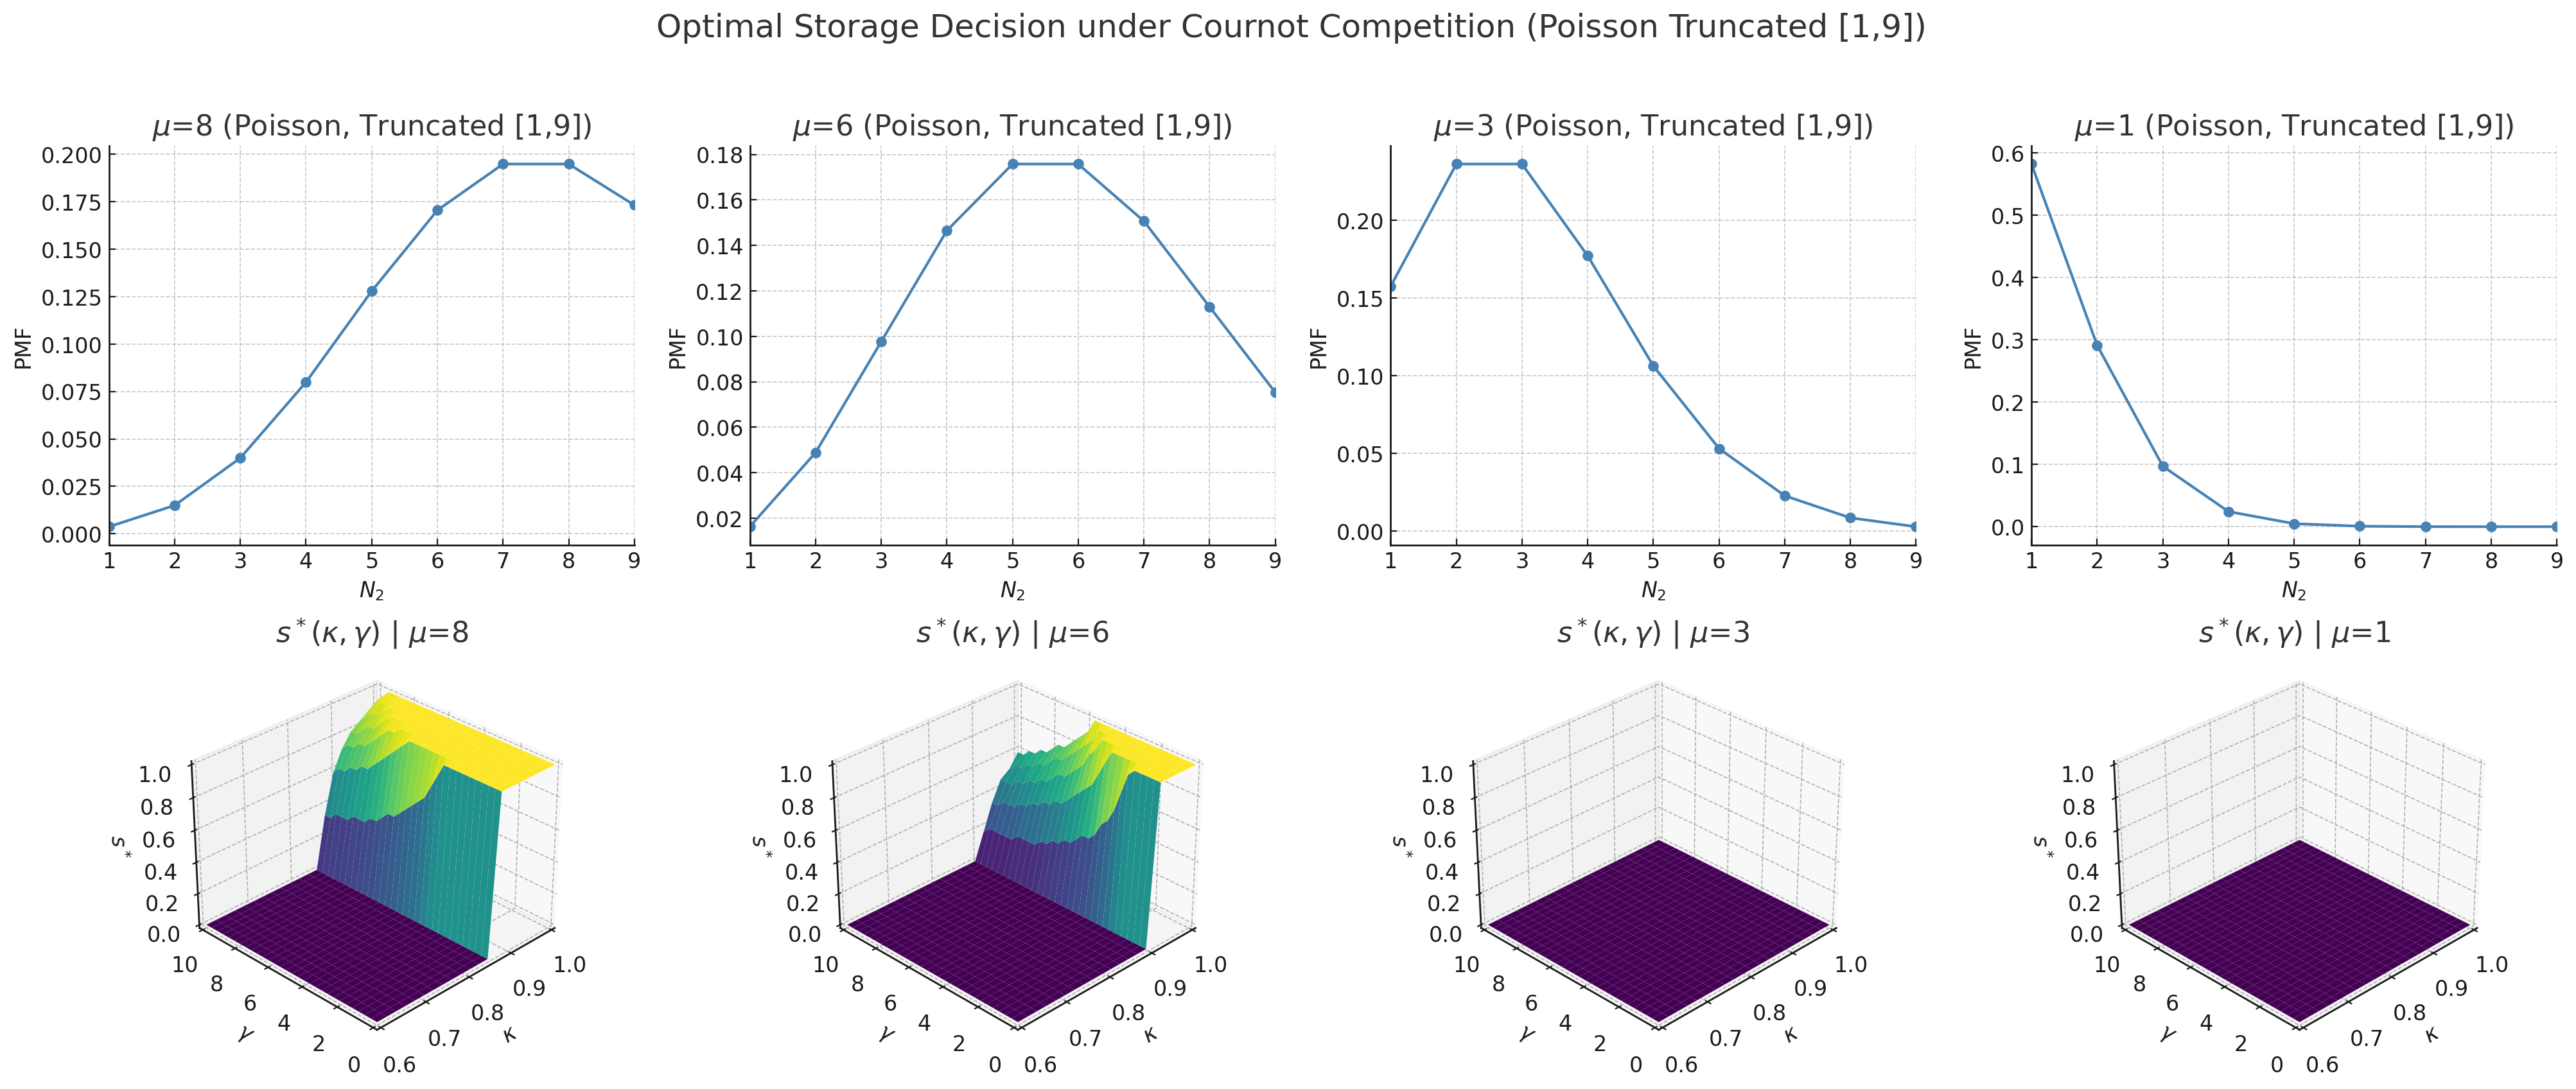
\includegraphics[width=\textwidth, keepaspectratio=true]{model_figures/3D_cournot.png}
        \caption{Optimal Storage Share and PDF Visualizations under Four Poisson Distributions of $N_2$}
        \label{Fig: 3D Cournot}
    \end{subfigure}
    
    \vspace{10mm} % Reduced vertical gap between subfigures
    
    \begin{subfigure}{\textwidth}
        \centering
        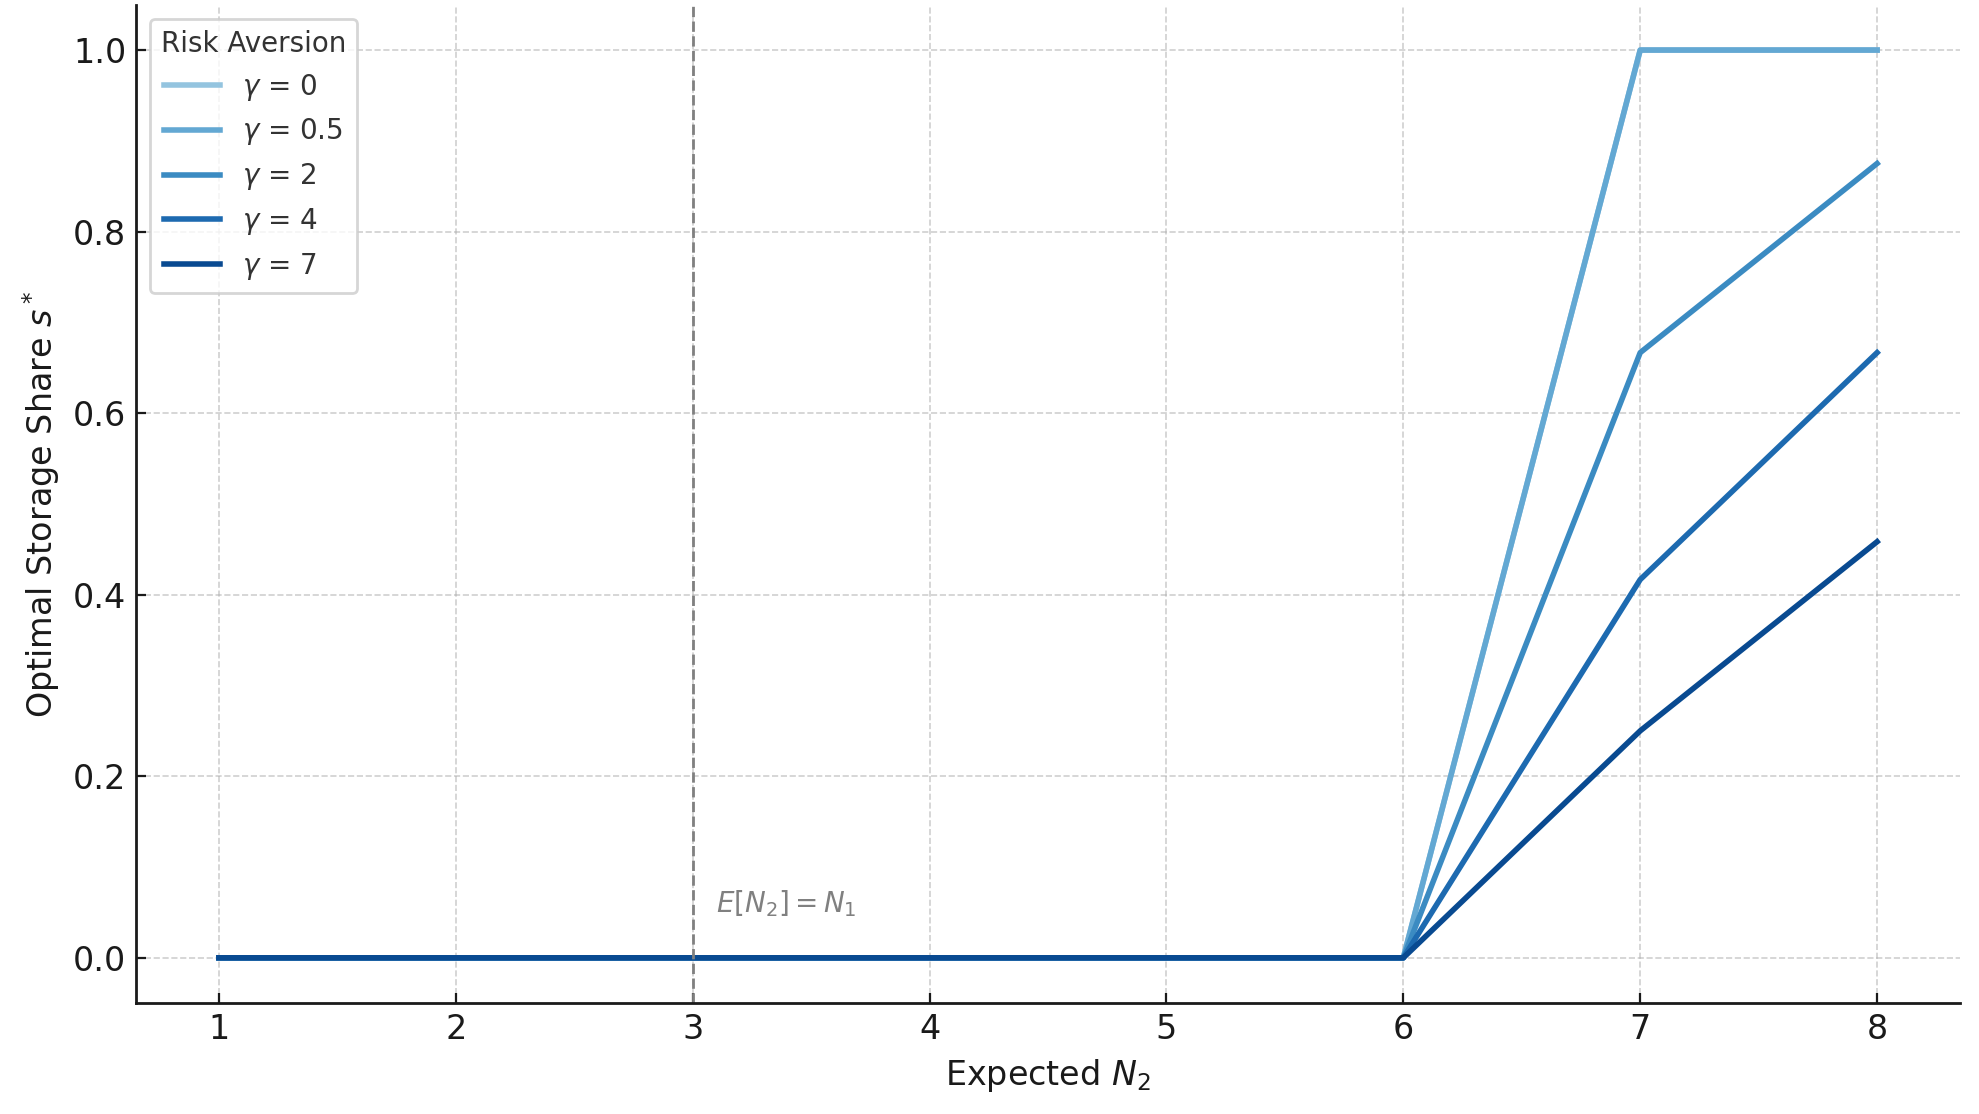
\includegraphics[width=\textwidth, keepaspectratio=true]{model_figures/buyer_count_sensitivity_cournot.png}
        \caption{Sensitivity to Expected Second-Period Buyer Presence ($\kappa=0.9$)}
        \label{Fig: Cournot sensitivity}
    \end{subfigure}

    \caption{Numerical Analysis under Cournot Competition}
\end{figure}



Figure~\ref{Fig: Cournot sensitivity} presents a three-panel sensitivity analysis of farmers' optimal storage share $s^*$ under Cournot competition when the second-period number of buyers follows a truncated Poisson distribution on $[0,9]$. The horizontal axis in each panel reports the expected value of $N_2$, and the vertical axis shows the corresponding optimal storage share. Each curve traces $s^*$ for a different level of risk aversion $\gamma \in \{0,0.5,2,4,7\}$, with darker shades of blue indicating higher $\gamma$. A vertical dashed line marks the benchmark case where the expected number of second-period buyers equals the observed first-period value, $\mathbb{E}[N_2]=N_1=3$. The three panels vary the assumed reservation price floor, $p_{\mathrm{reserve}} \in \{0.10,0.25,0.40\}$, which represents the outside option available if no standard buyers are present. This design allows direct comparison of how the outside option shifts storage incentives across risk preferences and market competitive scenarios.

Introducing a reservation price $p_{\text{reserve}}$ shifts the whole schedule upward in a economically intuitive way. A better fallback (from $0.10$ to $0.25$ to $0.40$) weakly lowers the threshold $\mathbb{E}[N_2]$ at which storage becomes attractive and increases $s^*$ at any given $\mathbb{E}[N_2]$-with the effect most pronounced for high $\gamma$, because the floor insures the downside of thin buyer markets. In short: more expected buyers and a stronger outside option both raise the optimal storage share, while greater risk aversion tempers that response.

On any particular curve plot in Figure~\ref{Fig: Cournot sensitivity}, increases in the expected second-period buyer count improve the attractiveness of storage. However, this does not always translate into a smooth rise in $s^*$: over a wide range of values for $N$, especially under high risk aversion, the optimal storage share remains at zero. Only once market prospects become sufficiently favorable does $s^*$ begin to increase, with less risk-averse farmers responding more readily to such improvements.


A key insight is that even under relatively favorable conditions-such as a low composite storage cost ($\kappa = 0.9$) and a moderately competitive harvest market ($N_1 = 3$)-storage becomes an attractive option only when farmers anticipate a substantially more buyer-presence market in the second period. Specifically, storage is only worthwhile when the expected number of buyers in period 2 reaches or exceeds 6, implying an expected price increase from $p_1 = \frac{3}{4} = 0.75$ to $p_2 = \frac{6}{7} \approx 0.857$. This 10.7 percentage point gain is sufficient to offset the 10\% effective loss due to storage inefficiency.


This result reflects the concave nature of the price function $p(N) = \tfrac{N}{N+1}$: as $N$ increases beyond 3, marginal improvements in price diminish. Therefore, even risk-neutral farmers require a strongly optimistic expectation of increased buyer presence to justify intertemporal arbitrage through storage. 

By contrast, when $N_1$ is very small (e.g., 1 or 2), the incremental price gains from attracting just one or two additional traders are much larger. For instance, moving from $N_1=1$ to $N_2=2$ raises the farm-gate price from $p_1=\tfrac{1}{2}=0.50$ to $p_2=\tfrac{2}{3}\approx 0.67$, while moving from $N_1=2$ to $N_2=3$ increases it further to $p_2=\tfrac{3}{4}=0.75$. Such discrete jumps can be large enough to incentivize storage. Thus, the stark threshold effect documented above is most relevant when the harvest market already exhibits moderate competition.




%----------------------------------------------------%
%----------------------------------------------------%



\section{Aggregate Welfare Simulation}\label{subsec:agg_welfare}
\noindent
This section shifts from the simulation analysis of individual storage decisions (Sections~\ref{Section: Base Model Numerical Analysis} to \ref{Section: Special Cases: Explicit Competition Forms}) to aggregate welfare. A central implication of our base storage-decision model is that policies which reduce the effective cost of storage can generate direct income and welfare gains. To formalize this insight, I extend the baseline framework by allowing both first- and second-period buyer power to be stochastic. In this environment, farmers' incentives to store depend not only on realized first-period and expected second-period prices but also on their heterogeneous attitudes toward risk and patience. I therefore construct a simulated ``village'' of farmers who are identical in production but only vary in risk preferences, and analyze how shifts in the storage efficiency parameter $\kappa$---interpretable as policy-driven reductions in storage costs, improvements in storage technology or lower farmer discount rates---translate into higher expected incomes and certainty-equivalent welfare.



\subsection{Simulation Process}
\noindent 
The objective is to simulate how optimal storage translates into aggregate welfare relative to a no-storage benchmark across a range of competitive conditions and storage-cost environments. Welfare is measured by (i) the percentage change in average village income and (ii) the percentage change in certainty equivalent (CE), computed under farmer risk preferences and then aggregated and averaged.

\paragraph{Environments and buyer power.}
Buyer power in periods 1 and 2, denoted $\theta_1$ and $\theta_2$, is modeled as Beta-distributed with a common variance $\sigma^2$ but distinct means $\mu_1$ and $\mu_2$. For each $(\mu,\sigma^2)$ pair, I parameterize $\theta\sim\text{Beta}(\alpha,\beta)$ using the mean-variance mapping,\footnote{For Beta distributions, each admissible mean-variance pair corresponds uniquely to a pair $(\alpha,\beta)$.} imposing \emph{strict feasibility}: $\alpha>0$ and $\beta>0$, equivalently $\sigma^2<\mu(1-\mu)$. Expectations about future competition are encoded by a mean gap $g\in\{0.00,0.05,0.15\}$, such that $\mu_2=\mu_1-g$. This enables the simulation to depict settings wherein farmers might rationally anticipate an improvement in period 2 competitive conditions for reasons that were discussed earlier in this chapter.

Storage policy is varied through efficiency levels $\kappa\in\{0.95,0.90,0.85,0.80\}$, while uncertainty is captured by variances $\sigma^2\in\{0.02,0.05,0.10,0.15\}$. For each $(\sigma^2,g)$ combination, $\mu_1$ is swept over a $0.05$ grid, subject to the feasibility requirement that both $(\mu_1,\sigma^2)$ and $(\mu_1-g,\sigma^2)$ remain admissible. Feasible mean intervals for each variance are documented in Figure~\ref{fig:parameter_range_Beta_distribution}.

\begin{figure}[ht!]
    \centering
    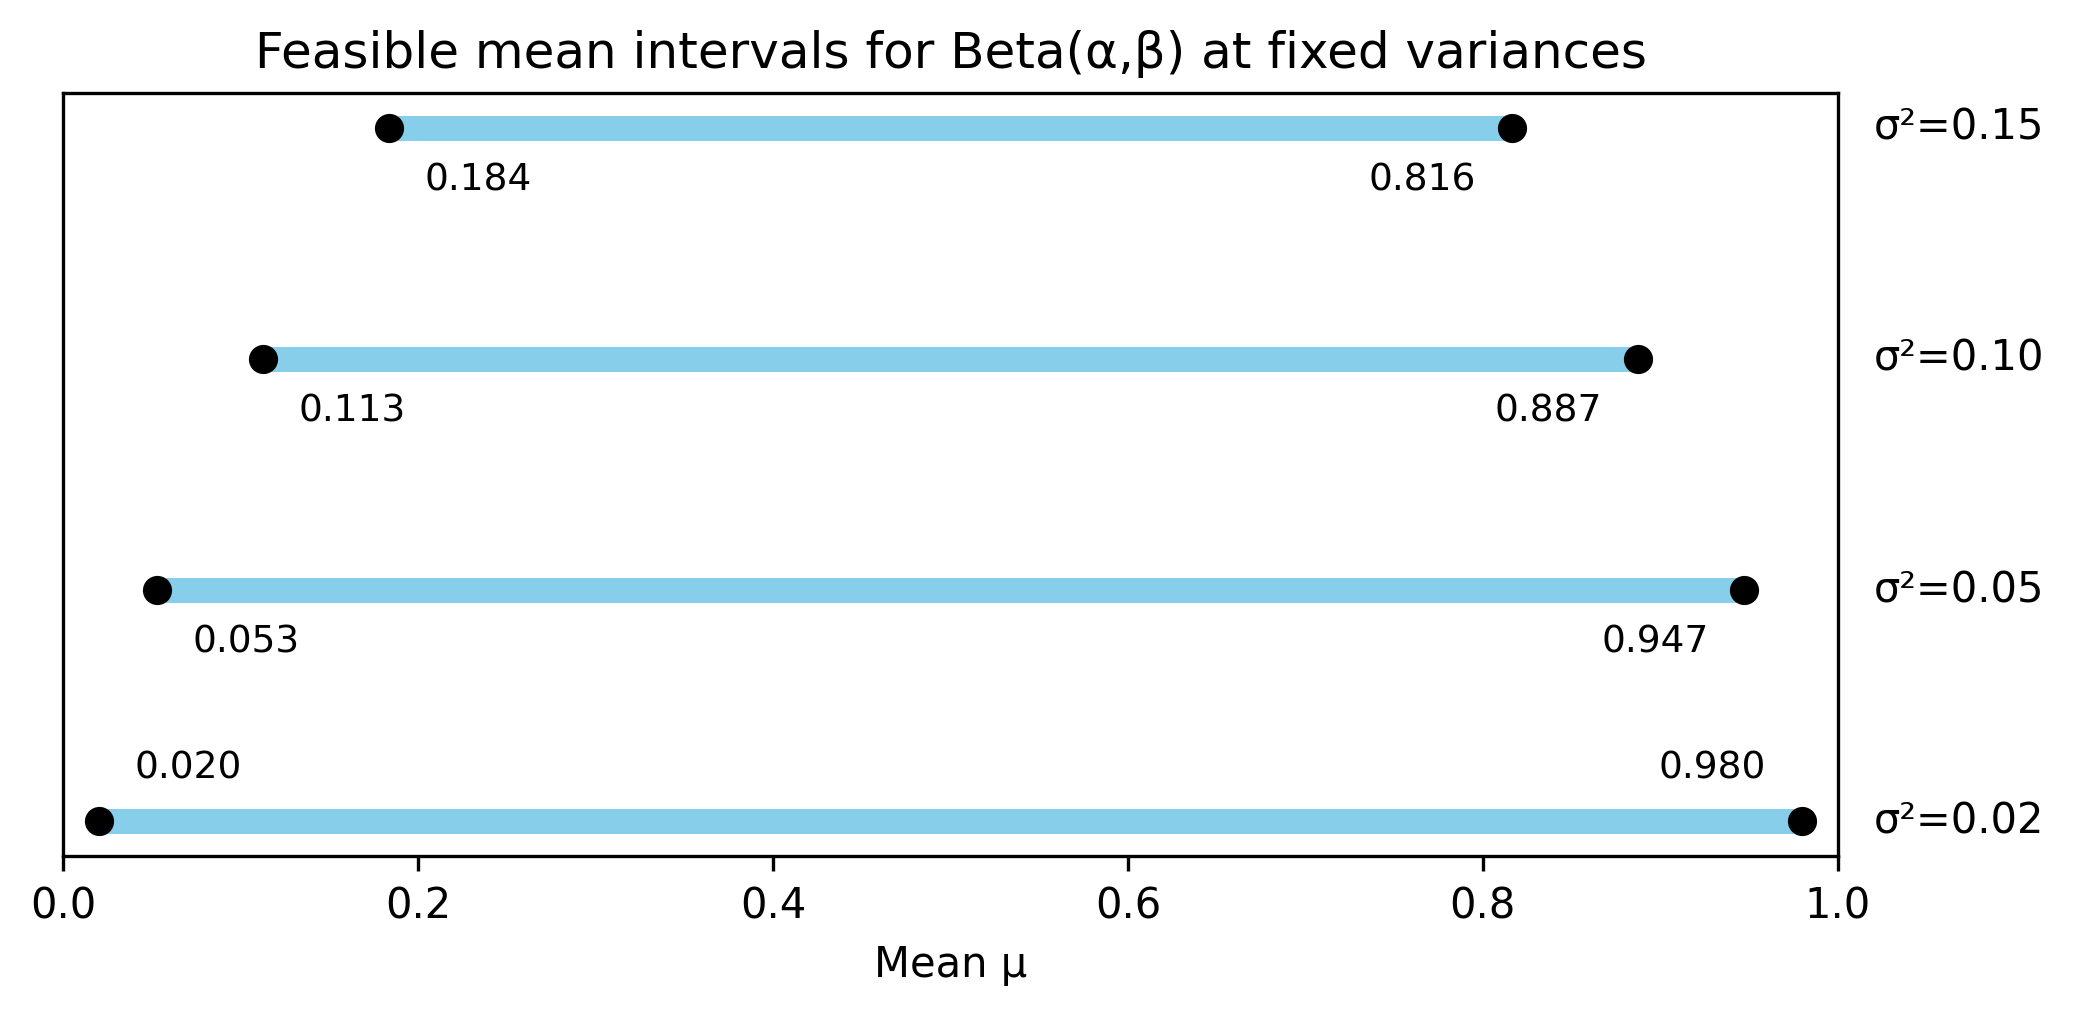
\includegraphics[width=0.90\linewidth]{model_figures/parameter_range_Beta_distribution.png}
    \caption{Feasible Mean Intervals for Beta Distributions at Fixed Variances}
    \label{fig:parameter_range_Beta_distribution}
\end{figure}

Figure~\ref{fig:beta_pdf_cdf_grid} displays Beta probability density functions (top) and cumulative distribution functions (bottom) for four alternative variance levels specified above. Within each panel, curves correspond to four alternative means, $\mu \in \{0.2, 0.4, 0.6, 0.8\}$, with darker shades representing higher means.


\begin{figure}[ht!]
    \centering
    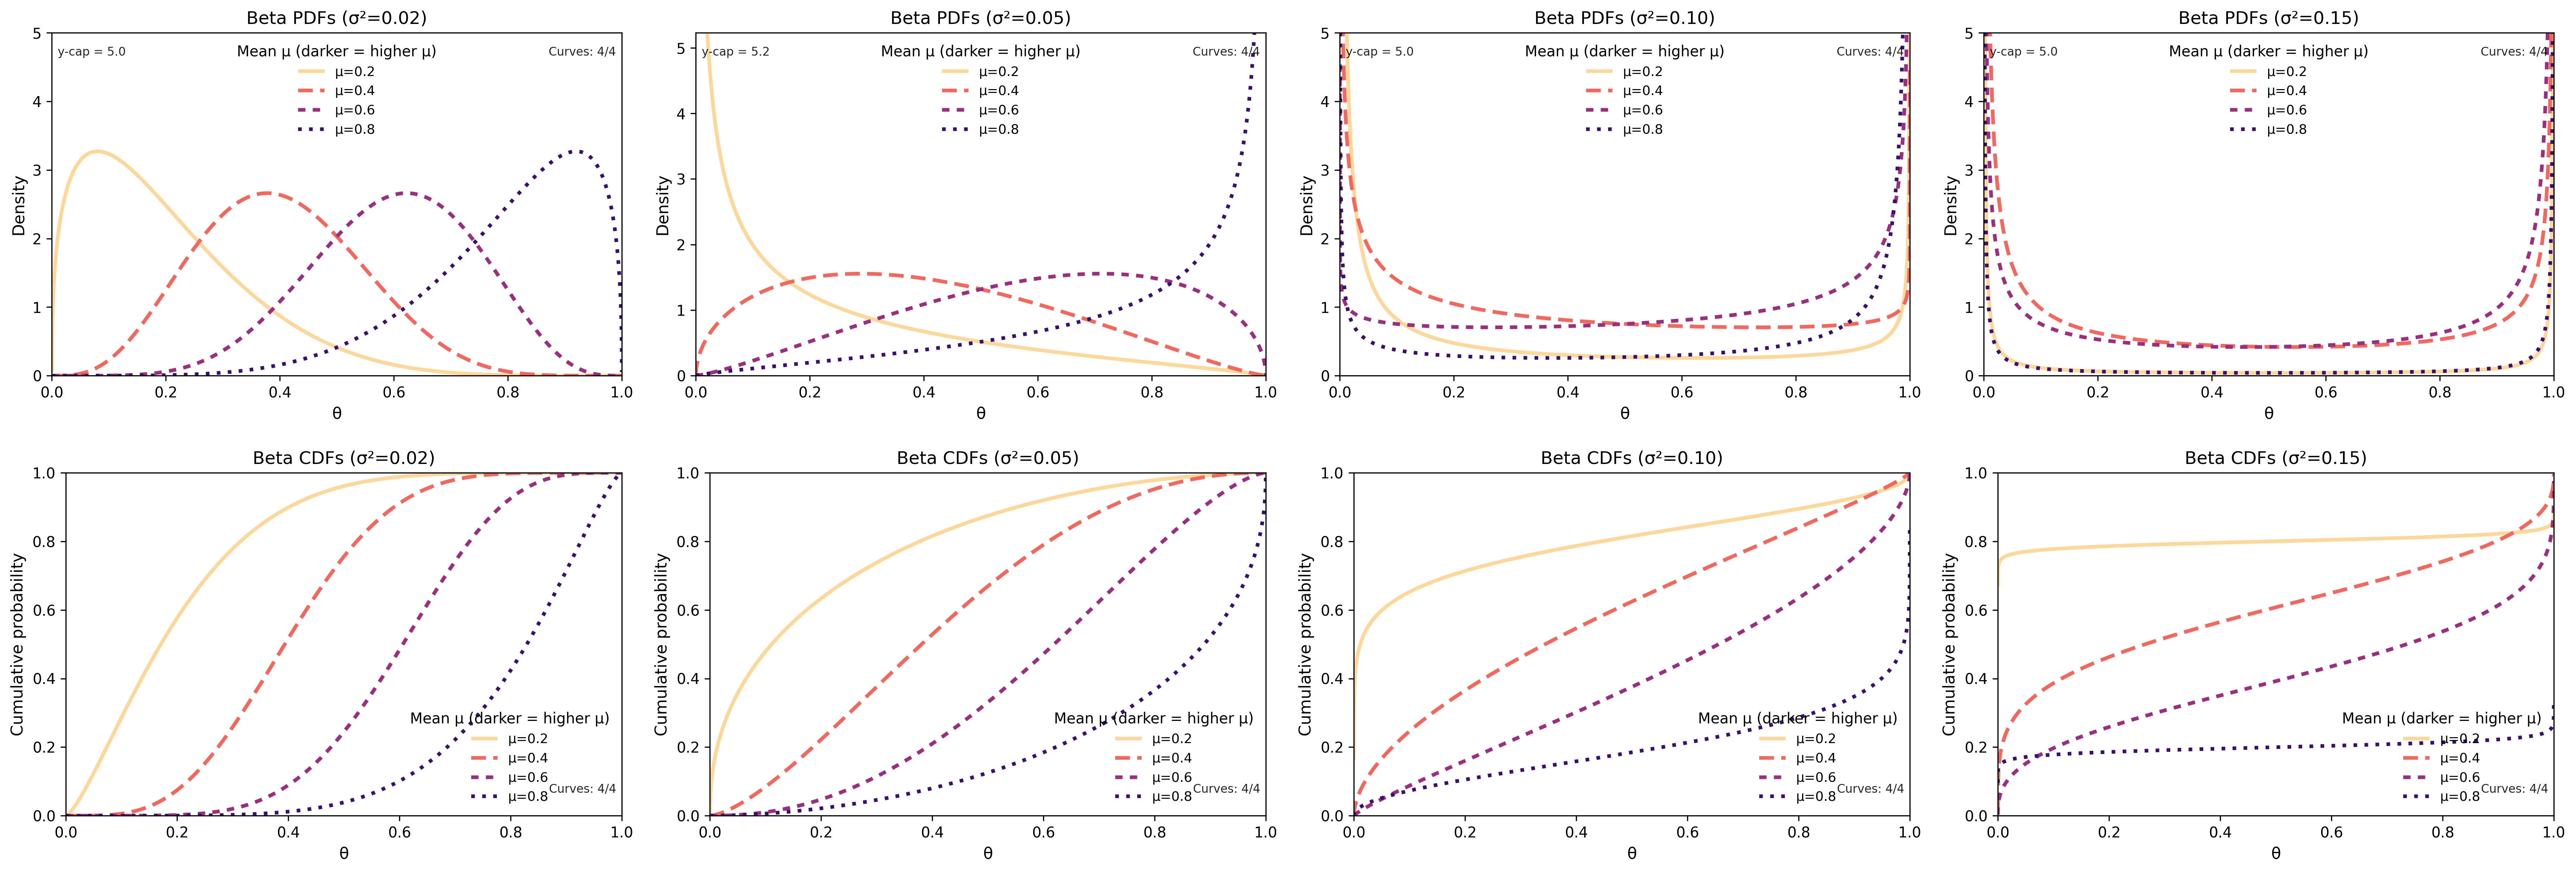
\includegraphics[width=\linewidth]{model_figures/beta_dist_PDF_CDF_grid_2x4.png}
    \caption{Beta Distributions with Alternative Means and Variances}
    \label{fig:beta_pdf_cdf_grid}
\end{figure}



\paragraph{Individual decision and numerical solution.}
The simulated village consists of $N=100$ farmers with CRRA preferences who differ only in risk aversion coefficient $\gamma_i\sim \mathrm{Uniform}[0,10]$ (drawn once and held fixed).

For a given $(\theta_1,\text{dist}(\theta_2),\kappa,\gamma)$, each farmer's optimal share $s^*(\theta_1,\gamma)$ solves
\[
\max_{s\in[0,1]} \; \mathbb{E}_{\theta_2}\!\left[\,U\!\big((1-s)p_1+s\,\kappa\,p_2\big)\right],
\qquad p_t=\frac{1}{1+\theta_t}.
\]
Expectations over $\theta_2$ are evaluated by 12-point Gauss--Legendre quadrature mapped to the Beta distribution. The one-dimensional problem is solved by golden-section search. To economize on computation, for each $\kappa$ and $(\mu_2,\sigma^2)$, I precompute $s^*$ on a $30\times 30$ grid in $(\theta_1,\gamma)$ and bilinearly interpolate for arbitrary realizations of $\theta_1$.\footnote{When $\gamma\approx 0$, I use the standard risk-neutral shortcut: $s^*\in\{0,1\}$ depending on whether $\kappa\,\mathbb{E}[p_2]>p_1$.}

\paragraph{World simulation and aggregation.}
For every triplet $(\mu_1,\sigma^2,g)$, I simulate $R=20{,}000$ worlds.\footnote{I fix random seeds for reproducibility and (where applicable) reuse common random numbers across $\mu_1$ within a given $(\sigma^2,g)$ to improve comparability.} In world $r$, $(\theta_{1r},\theta_{2r})$ are drawn from their Beta distributions. Each farmer $i$ observes $\theta_{1r}$, knows the distribution of $\theta_2$, and determines the optimal storage share, $s^*_i(\theta_{1r},\gamma_i)$. Realized income is
$$
y_{ir}=(1-s^*_{ir})\,p(\theta_{1r})+s^*_{ir}\,\kappa\,p(\theta_{2r}).
$$
I aggregate to the \emph{village mean} in each world, $\bar y_r=\frac{1}{N}\sum_i y_{ir}$. The no-storage benchmark in world $r$ is $\bar y^{\,\text{no}}_r=\frac{1}{N}\sum_i p(\theta_{1r})$.



\paragraph{Income gain metric.}  
To quantify the effect of storage opportunities on farm revenues, I first construct a percentage income gain measure. For a given environment $(\kappa,\sigma^2,g)$ and initial mean $\mu_1$, the expected average income with storage, relative to the no-storage benchmark, is  
\begin{equation}
\text{Expected Income Gain}(\mu_1;\kappa,\sigma^2,g)
=100\times
\frac{\frac{1}{R}\sum_{r=1}^R \bar y_{r}-\frac{1}{R}\sum_{r=1}^R \bar y^{\,\text{no}}_{r}}
{\frac{1}{R}\sum_{r=1}^R \bar y^{\,\text{no}}_{r}}.
\end{equation}
This measure captures the average proportional improvement in farm income arising from intertemporal arbitrage: farmers allocate harvests across periods to exploit expected price improvements, net of composite storage costs. The magnitude reflects both the degree of price variability and the distributional assumptions on buyer power.



\paragraph{Certainty–equivalent (CE) metric.}  
Because risk preferences are central to farmer welfare, I complement the income-based comparison with a certainty-equivalent (CE) measure grounded in CRRA utility. For farmer $i$, expected utility is computed as  
\begin{equation}
\mathrm{EU}_i
=\frac{1}{R}\sum_{r=1}^R U(y_{ir};\gamma_i),
\end{equation}
where $\gamma_i$ denotes the coefficient of relative risk aversion. Using the closed-form inverse of CRRA utility, the farmer-level CE income is  
\begin{equation}
\mathrm{CE}_i=
\begin{cases}
\left(\frac{1}{R}\sum_{r=1}^R y_{ir}^{\,1-\gamma_i}\right)^{\!\!\tfrac{1}{1-\gamma_i}}, & \gamma_i\neq 1,\\[8pt]
\exp\!\left(\frac{1}{R}\sum_{r=1}^R \ln y_{ir}\right), & \gamma_i=1.
\end{cases}
\end{equation}
The village-level CE is then the equal-weight mean across all farmers,  
$$
\overline{\mathrm{CE}}=\frac{1}{N}\sum_{i=1}^N \mathrm{CE}_i.
$$
An analogous benchmark, $\overline{\mathrm{CE}}^{\,\text{no}}$, is computed under the no-storage outcome $y^{\text{no}}_{ir}=p(\theta_{1r})$. The welfare change from adopting storage is expressed as  
\begin{equation}
\mathrm{CE\text{-}Gain}(\mu_1;\kappa,\sigma^2,g)
=100\times
\frac{\overline{\mathrm{CE}}-\overline{\mathrm{CE}}^{\,\text{no}}}{\overline{\mathrm{CE}}^{\,\text{no}}}.
\end{equation}

By construction, the certainty equivalent for any given risky policy satisfies $\mathrm{CE}_i<\mathbb{E}[y_i]$ for risk-averse farmers.  
However, when comparing two policies---such as optimal storage versus selling immediately---the difference in CE can exceed the difference in mean income.  
This occurs because  
$$
\Delta \mathrm{CE}
=\Delta \mathbb{E}[y]
-\Delta \mathrm{RP},
\text{ where }
\mathrm{RP}=\mathbb{E}[y]-\mathrm{CE},
$$
and the simulations below indicate $\Delta \mathrm{RP}<0$. The mechanism is insurance: the state-contingent mix $(1-s)p_1 + s\kappa p_2$ has lower variance than $p_1$ because $(1-s)^2 + (s\kappa)^2 < 1$ for $\kappa < 1$ and $s \in (0,1)$. Optimal choices concentrate storage in low-price states, truncating downside tails and dampening upside exposure, which reduces the risk premium.

In other words, compared with no-storage benchmark, storage not only changes expected revenue but also lowers income variance and thus the risk premium. Optimal storage shares act like a portfolio between current and future prices, which compresses outcome dispersion.  

Therefore, the CE-Gain measure captures both the rise in mean income and the sizable ``insurance dividend'' from risk smoothing, providing a richer welfare indicator than the income-gain metric alone.



\begin{figure}[ht!]
    \centering
    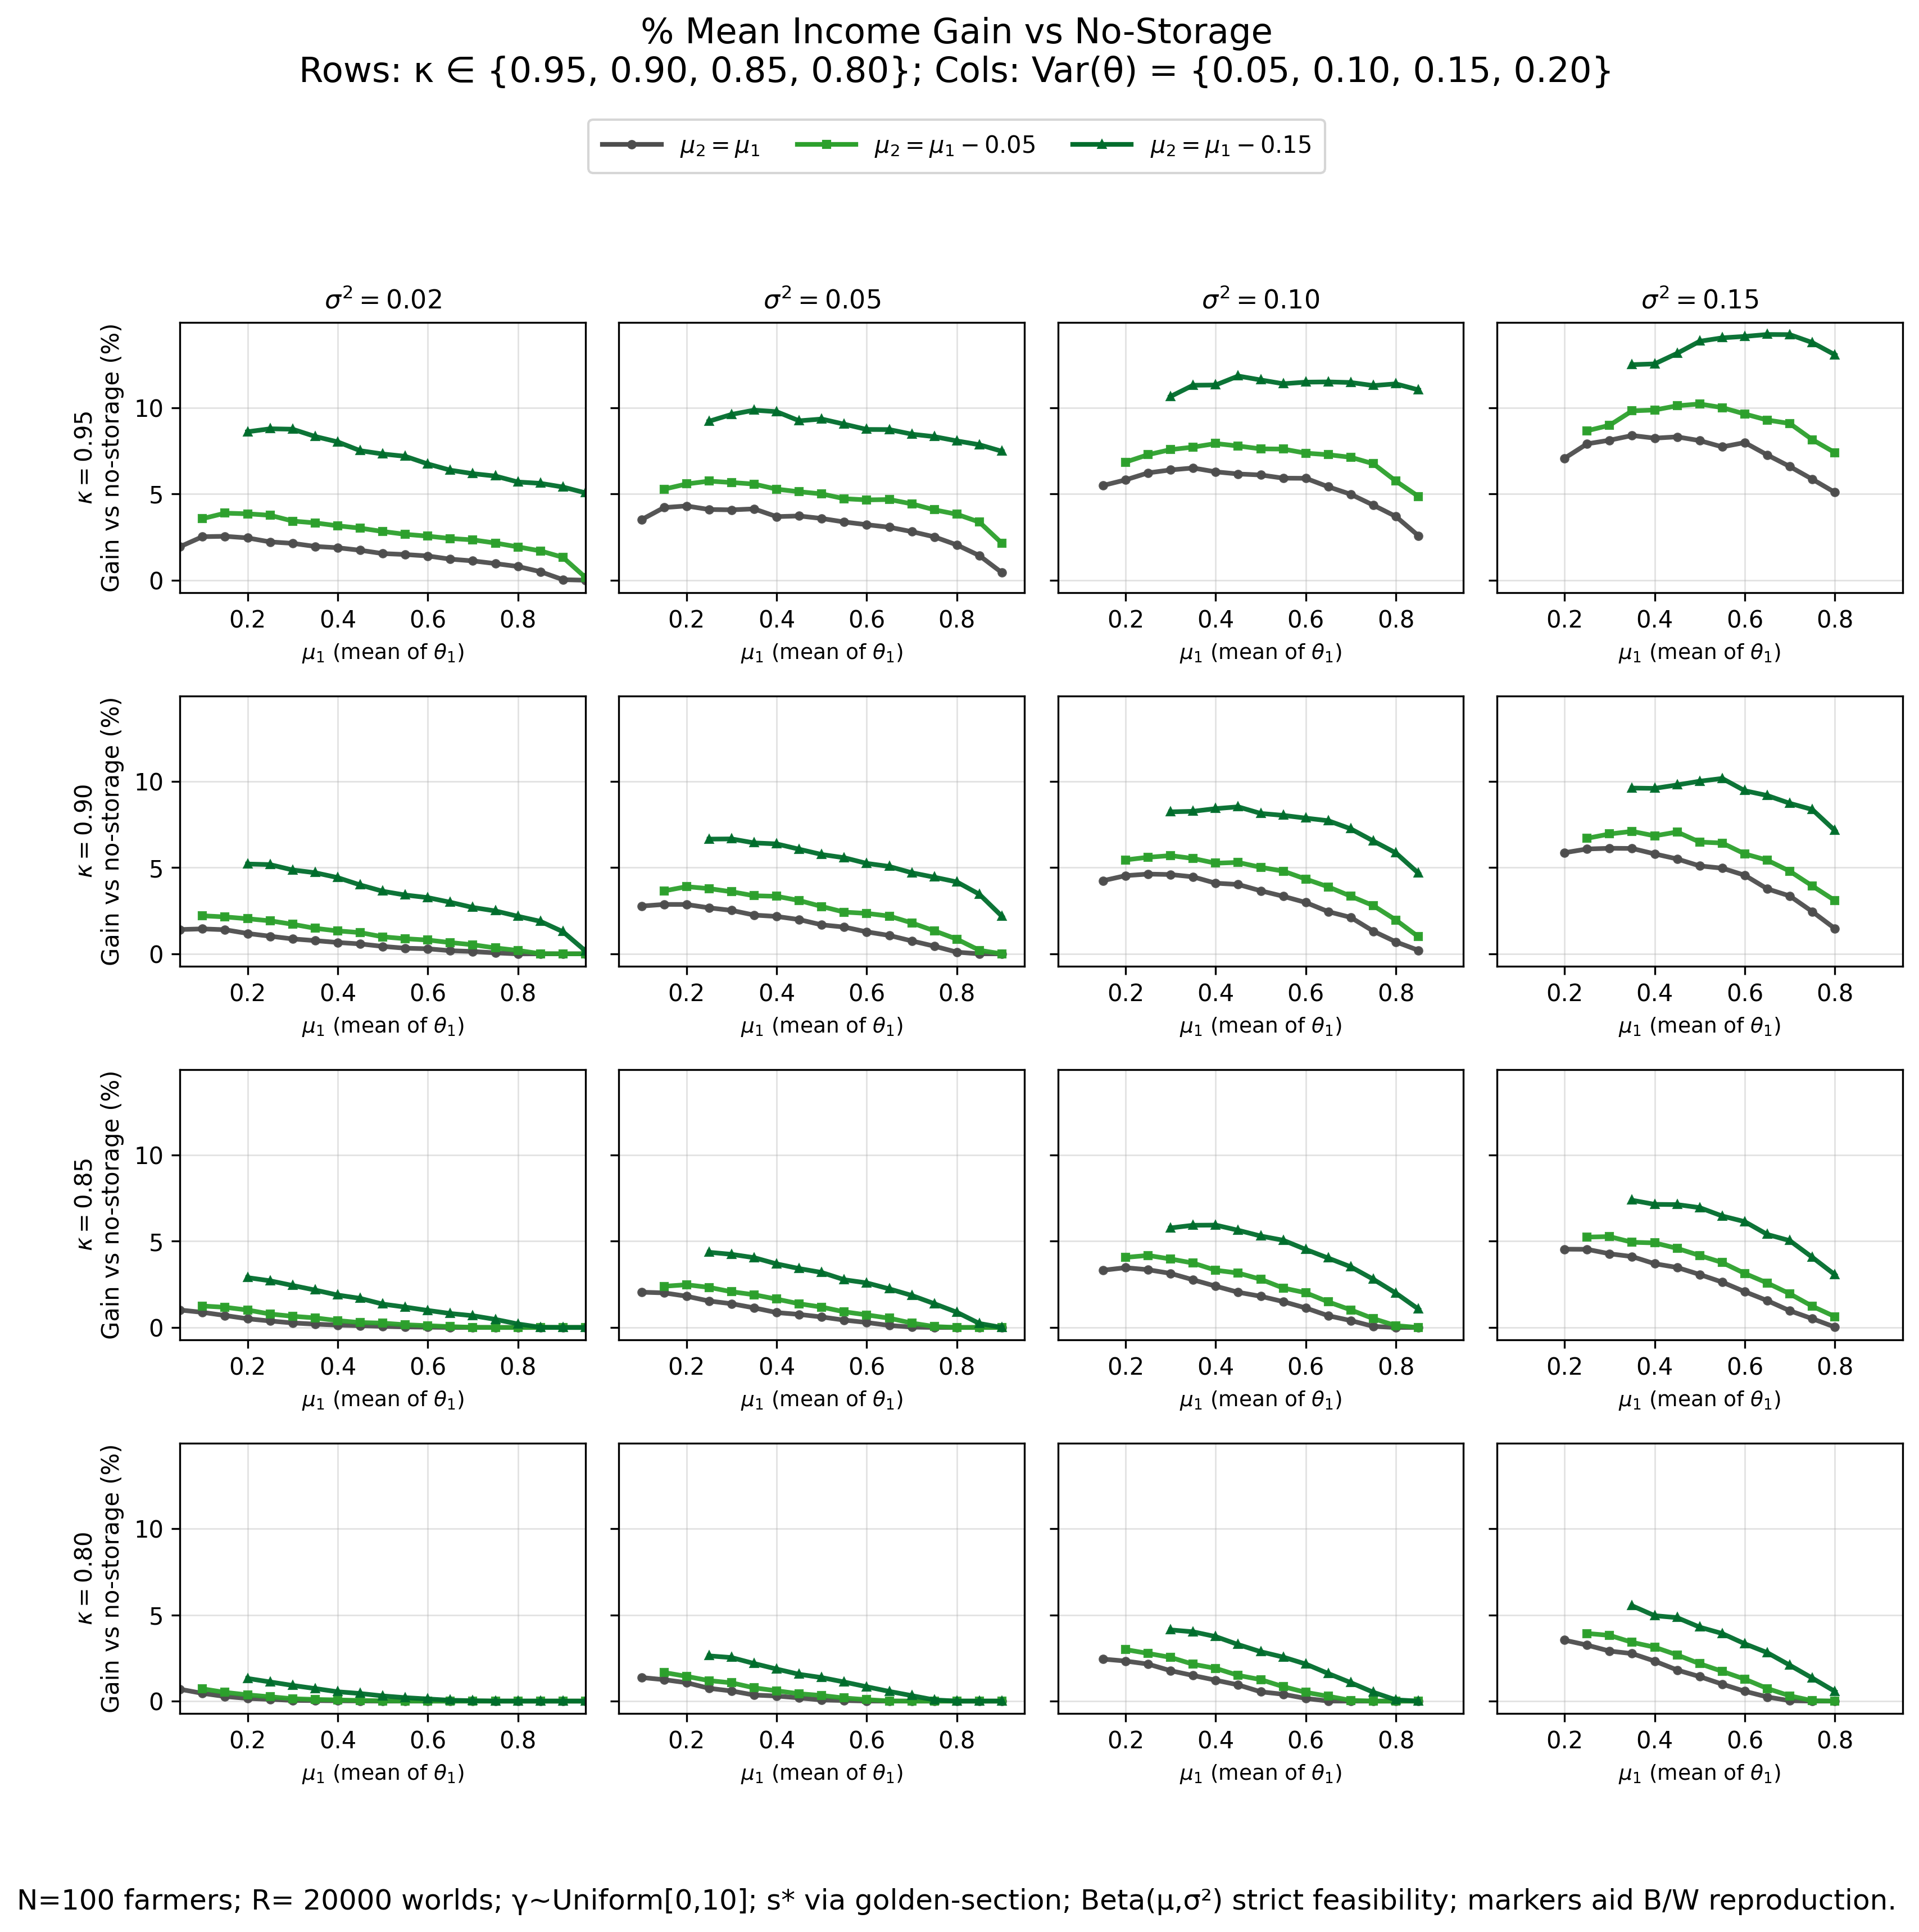
\includegraphics[width=\linewidth]{model_figures/gainpct_grid_4x4.png}
    \caption{Percent Mean Income Gain vs No-Storage}
    \label{fig: Income gains}
\end{figure}


\subsection{Welfare versus No-Storage Benchmark}
\noindent 
Figure~\ref{fig: Income gains} presents a $4\times4$ grid of panels that quantify percentage income gains from intertemporal storage relative to the no-storage benchmark. The design varies two key parameters. Along the vertical dimension, rows correspond to alternative storage efficiencies, $\kappa$, declining from 0.95 at the top to 0.80 at the bottom. Along the horizontal dimension, columns represent different levels of buyer-power uncertainty, with the variance parameter $\sigma^2$ increasing from 0.02 on the left (low uncertainty) to 0.15 on the right (high uncertainty). Within each panel, the horizontal axis reports the mean of first-period buyer power, $\mu_1$, while the vertical axis shows the average percentage income gain at the village level when storage is available.  

Each panel traces three curves that capture different expectations about second-period buyer power. The dark-gray line depicts $\mu_2=\mu_1$, implying a stable distribution across periods. The lighter green line represents $\mu_2=\mu_1-0.05$, while the darker green line reflects $\mu_2=\mu_1-0.15$. Both of these scenarios correspond to expectations of weaker buyer power in period 2, which in turn imply higher expected future prices. The vertical spread among curves therefore provides a measure of how sensitive welfare gains from storage are to changes in intertemporal beliefs.

\medskip
\noindent 
Several insights emerge from this set of panels:

\begin{enumerate}
    \item \textit{Storage Efficiency effect.} Across all levels of buyer-power uncertainty, higher storage efficiency translates directly into larger income gains. This manifests as an upward shift of the entire set of curves when moving from lower to higher values of $\kappa$. Put differently, technological improvements that reduce storage losses substantially magnify the welfare benefits from intertemporal arbitrage.  
    \item \textit{Role of intertemporal buyer power mean change.} When farmers can rationally anticipate weaker mean buyer power in the future, storage becomes systematically more profitable. The vertical distance between the dark-gray and green curves reveals the incremental gain from expecting higher second-period prices, with the gap widening as the expected deterioration in buyer power becomes more pronounced.  
    \item \textit{Impact of buyer power volatility.} Increasing variance in buyer power distributions raises all curves, reflecting the convexity of $p(\theta)=1/(1+\theta)$ and the option value of storage under uncertainty. The option to store has greater value under more volatile competitive environments. Greater variance also amplifies the differences across expectation scenarios, highlighting how risk interacts with beliefs to shape welfare outcomes.  
    \item \textit{Mean buyer power across periods.} Holding uncertainty/variance fixed, higher average first-period buyer power ($\mu_1$), as well as the associated second-period buyer power ($\mu_2$), generally reduces storage gains.  
    \item \textit{Non-monotonicity under certain conditions.} An important exception arises when storage efficiency is high and uncertainty is large. In these settings, the relationship between $\mu_1$ and storage gains becomes non-monotonic, taking the form of an inverted-U. This pattern indicates that modest levels of first-period buyer power create the greatest scope for welfare improvements from storage, whereas extremely high or extremely low buyer power attenuates the relative benefit.
\end{enumerate}

\noindent 
A closely related design underlies Figure~\ref{fig:CE gains}, which reports certainty-equivalent (CE) gains relative to the no-storage benchmark. The qualitative patterns largely mirror those for expected income gains: higher storage efficiency, more favorable expectations about future buyer power, and greater market uncertainty all reinforce the value of storage. One important difference, however, emerges in the role of mean buyer power across periods. Whereas expected income gains can display a non-monotonic, inverted-U relationship with $\mu_1$ under high efficiency and uncertainty, CE gains decline monotonically in $\mu_1$ across all parameter configurations. This contrast highlights the disciplining role of risk aversion: once the curvature of utility is taken into account, farmers' welfare is consistently lower when buyer power is stronger in the first period, and the non-monotonicity observed for expected gains vanishes.

\paragraph{Policy lessons.} 
The simulation suggests a straightforward prioritization of generic ``enable-storage'' investments toward contexts where they yield the greatest welfare gains. First, raising storage efficiency ($\kappa$) is universally beneficial and should be the backbone of policy. Second, when decisions are guided by expected income, prioritize locales with nontrivial buyer-power volatility ($\sigma^2$) and middling first-period buyer power ($\mu_1$); uncertainty raises the option value of storage and moderate $\mu_1$ maximizes incremental gains. Third, once welfare is assessed through certainty equivalents, the non-monotonicity disappears and CE gains decline in $\mu_1$, implying a shift in priority toward areas with lower $\mu_1$. Finally, because expected gains rise when farmers anticipate weaker future buyer power ($\mu_2<\mu_1$, i.e., higher expected future prices), complementary policies that enhance buyer competition---thereby credibly tilting intertemporal beliefs---further amplify the payoff to storage investments.





\begin{figure}[ht!]
    \centering
    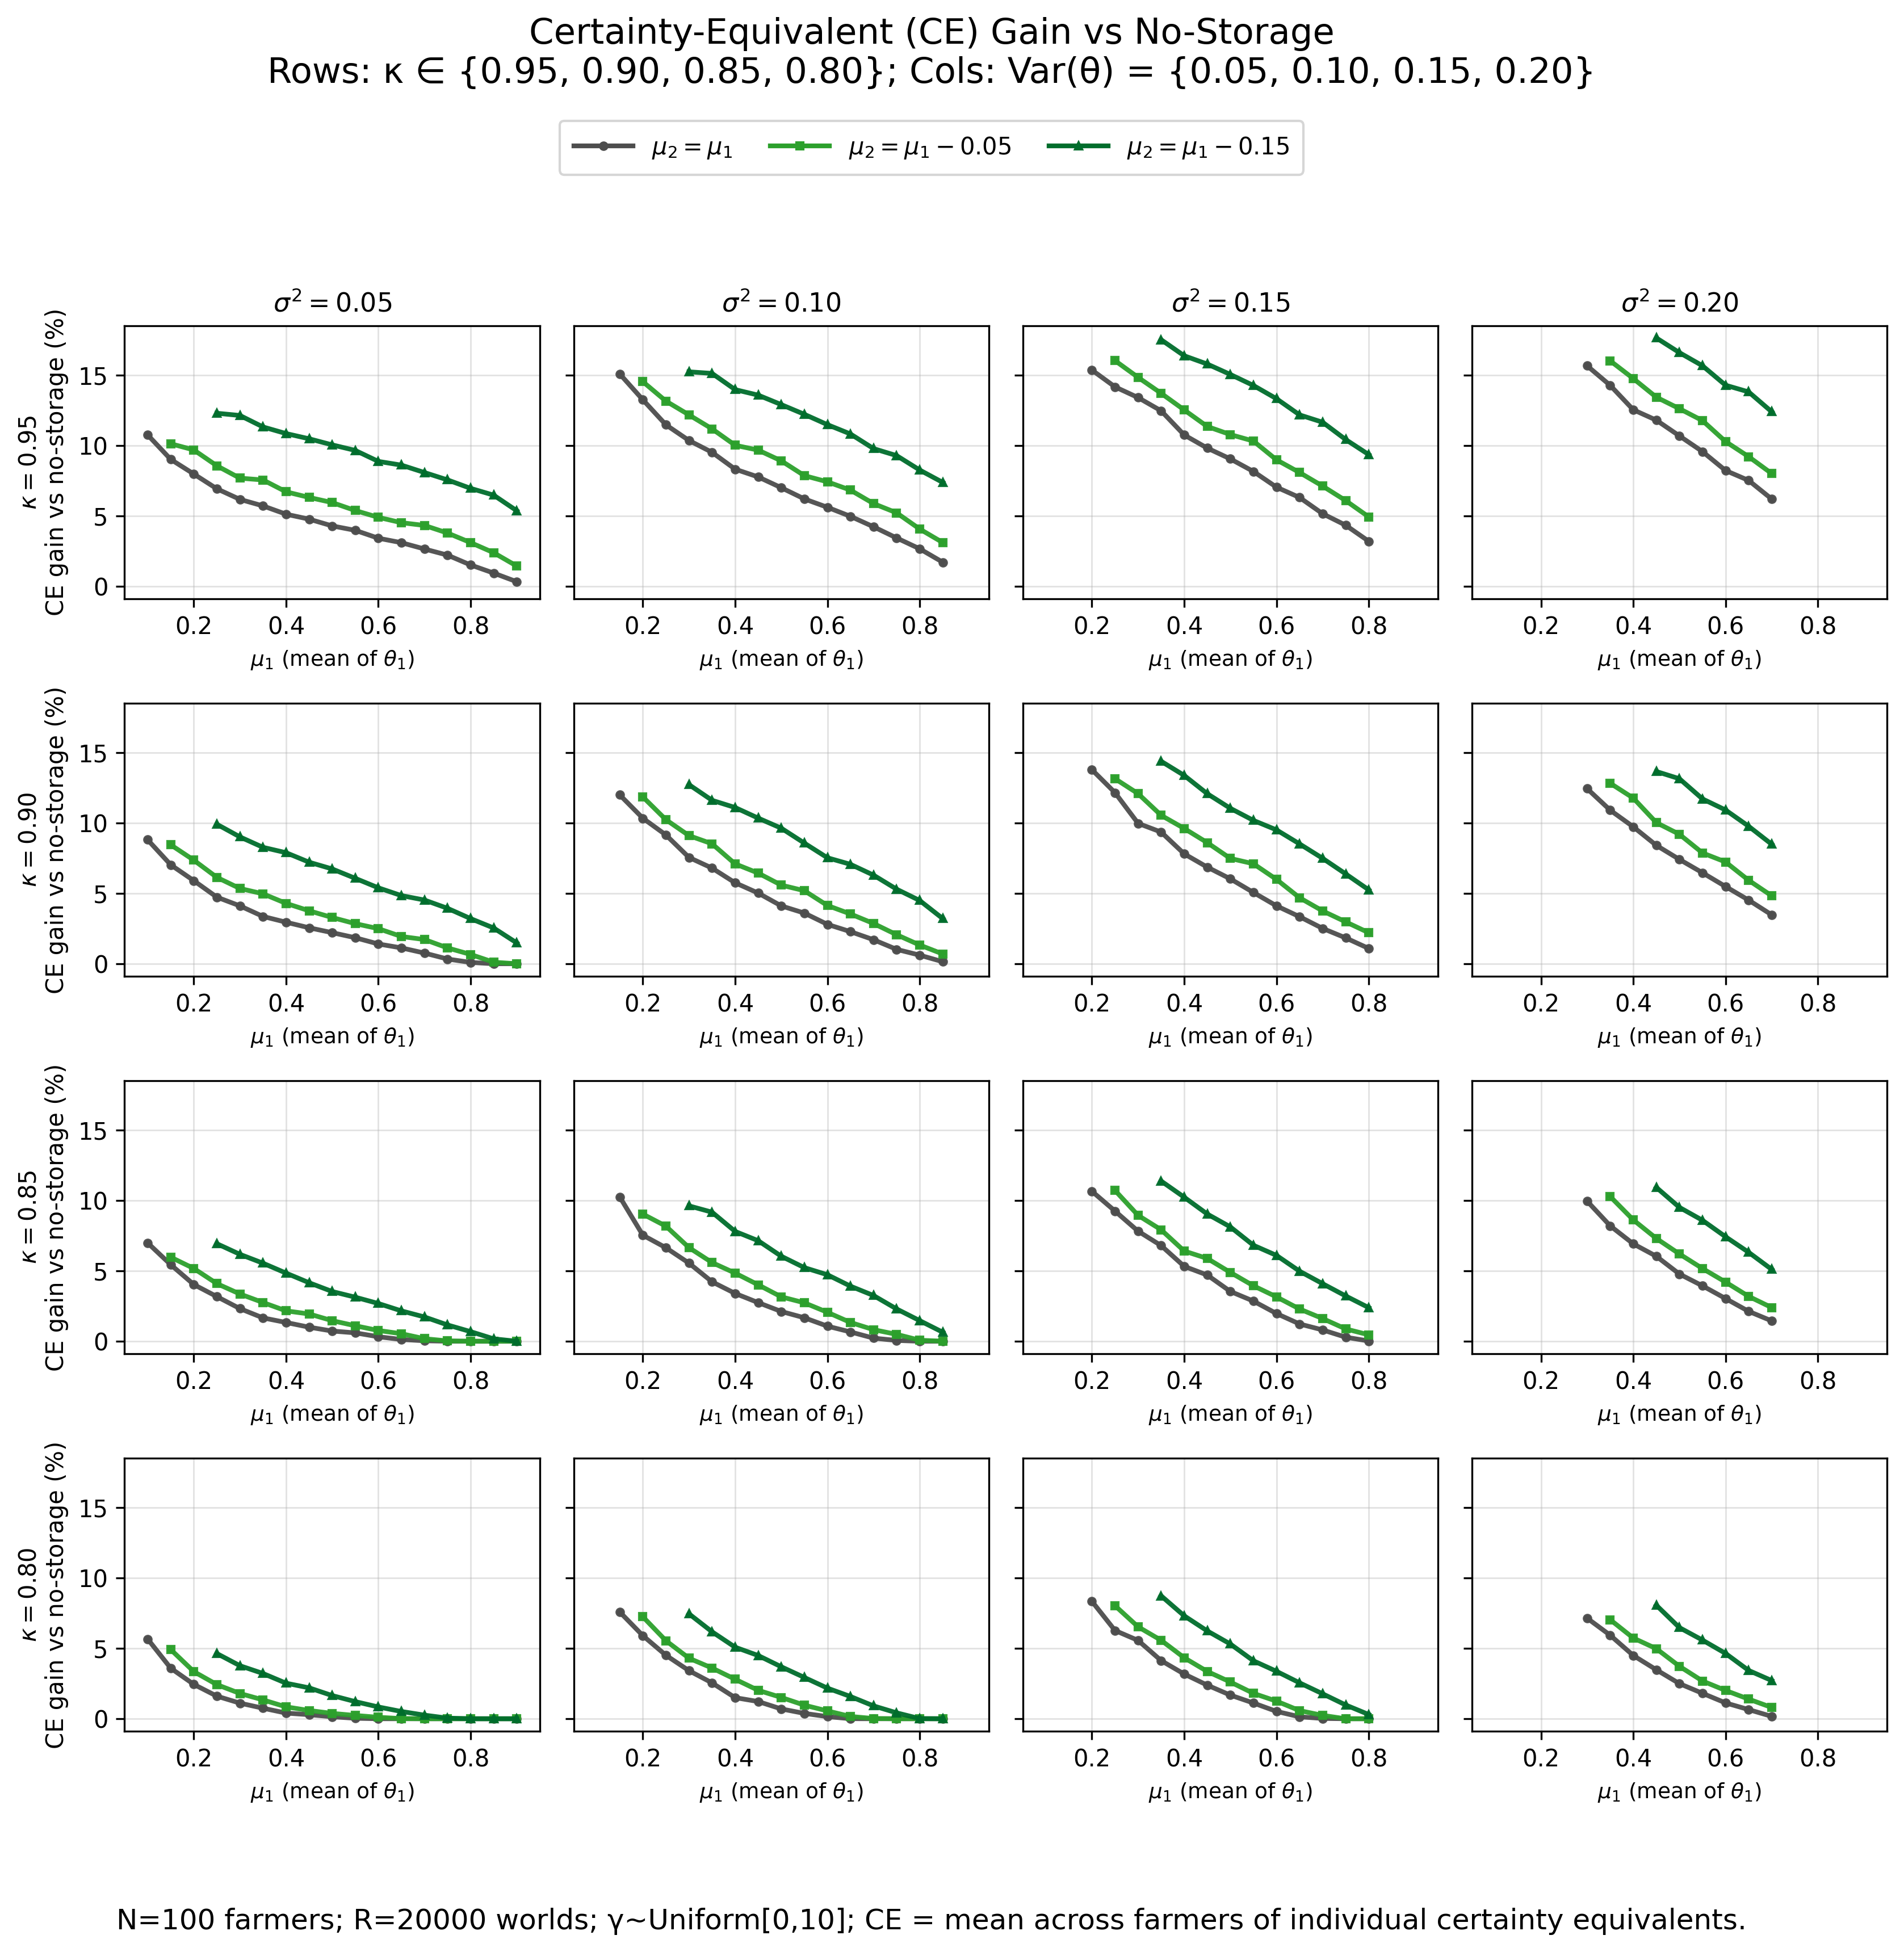
\includegraphics[width=\linewidth]{model_figures/cegain_grid_4x4.png}
    \caption{Percent Certainty-Equivalent Gain vs No-Storage}
    \label{fig:CE gains}
\end{figure}


\subsubsection{Why Inverted U shapes in some Expected-Income-Gain Curves?}
\noindent
Consider the risk--neutral benchmark ($\gamma=0$). The storage decision is binary: a farmer stores all or none depending on whether the discounted expected future price exceeds today's price. The farmer stores if
\[
\kappa\,\mathbb{E}\!\left[p(\theta_2)\right] \;>\; p(\theta_1), 
\qquad \theta_1,\theta_2\stackrel{i.i.d.}{\sim}\mathrm{Beta}\!\left(\alpha(\mu),\beta(\mu)\right),
\]
where $(\alpha(\mu),\beta(\mu))$ are the Beta-Distribution parameters associated with mean $\mu$ and variance $\sigma^2$.\footnote{Throughout, $\sigma^2$ is the variance target used to pin down $(\alpha,\beta)$ given $\mu$. ``Compactness'' refers to how concentrated the implied Beta density is under $(\alpha(\mu),\beta(\mu))$.}

Define the benchmark cutoff
\[
A(\mu)\;\equiv\; \kappa\,\mathbb{E}_{\mu}\!\left[p(\theta)\right], 
\quad \text{with } \theta\sim\mathrm{Beta}\!\left(\alpha(\mu),\beta(\mu)\right),
\]
and let $P_1=p(\theta_1)$ have cdf $F(\cdot;\mu)$ and density $f(\cdot;\mu)$. The expected gain relative to no storage is
\[
G(\mu) \;=\; \int_{0}^{A(\mu)} \big(A(\mu)-p\big)\,f(p;\mu)\,dp
\;=\; A(\mu)\,F\!\left(A(\mu);\mu\right)-\int_{0}^{A(\mu)} p\,f(p;\mu)\,dp,
\]
where the second equality follows by integration by parts. This representation makes clear that $G(\mu)$ is the area between the constant benchmark $A(\mu)$ and the (truncated) price distribution for $P_1$ up to $A(\mu)$.

\paragraph{Two forces behind the hump.}
Differentiating under the integral sign gives
\[
\frac{dG}{d\mu}
\;=\; A'(\mu)\,F\!\left(A(\mu);\mu\right)
\;+\; \int_{0}^{A(\mu)} \!\big(A(\mu)-p\big)\,\partial_{\mu} f(p;\mu)\,dp.
\]
The sign of $dG/d\mu$ reflects two distinct forces:

\medskip
\noindent\emph{(i) Curvature (marginal--gain) channel.} Since $p'(\theta)=-1/(1+\theta)^2<0$ and $p''(\theta)=2/(1+\theta)^3>0$, $p(\theta)$ is decreasing and convex. Decreasing $\theta$ (moving to lower buyer power) yields larger price gains when $\theta$ is low than when it is high. As $\mu$ rises, the distribution of $\theta$ shifts right, diminishing $\mathbb{E}[p(\theta)]$ and thus $A(\mu)$; formally $A'(\mu)<0$. This lowers $G(\mu)$ (the first term above). Intuitively, when buyer power is centered at low levels, the payoff to getting an even better draw in period~2 is large because of the convexity of $p(\cdot)$. As $\mu$ moves to higher buyer power, marginal price gains from an improvement in $\theta$ shrink.

\medskip
\noindent\emph{(ii) Compactness (probability--mass) channel.} The second term captures how the shape of the Beta distribution (hence the induced $P_1$ distribution) varies with $\mu$ for a given $\sigma^2$. For the variance ranges we use, the implied Beta tends to be relatively compact (concentrated) when $\mu$ is near the boundaries and more diffuse at moderate $\mu$. Holding the cutoff fixed, a more diffuse distribution places more mass below $A$, making it more likely that $p(\theta_1)$ falls under the benchmark and that storage pays. Thus, as $\mu$ increases from low to moderate values, the probability of realizing a meaningfully better second--period draw rises, raising $G(\mu)$.

\paragraph{Putting the channels together.}
These two forces move in opposite directions over the $\mu$ range, and with sufficiently high storage efficiency they may jointly generate an interior maximum. When $\mu$ is low, the curvature channel suggests that the payoff from an improvement in $\theta$ is large. However, the compactness channel works against it: with a tight Beta distribution concentrated near low $\mu$, the probability of drawing a substantially lower $\theta_2$ than $\theta_1$ is small. As a result, expected gains remain modest despite the large marginal payoff. As $\mu$ increases to moderate levels, the curvature channel weakens---marginal gains from better $\theta$ are smaller than when $\mu$ was low---but the compactness channel flips in favor of storage. The Beta distribution becomes more diffuse, boosting the probability of a materially better second--period draw. The higher likelihood of improvement dominates the smaller per--unit payoff, so $G(\mu)$ rises and reaches a peak. At high $\mu$, both channels suppress gains. The cutoff $A(\mu)$ collapses as $\mathbb{E}[p(\theta)]$ declines, while the Beta distribution again grows compact with most mass at high $\theta$. In this range, marginal gains from improving $\theta$ are small, and the chance of a large improvement is low. Consequently, $G(\mu)$ falls, completing the inverted-U shape.

The result is a potential inverted-U relationship between $G(\mu)$ and $\mu$, driven by the interaction of the \emph{convex} price mapping $p(\theta)$ and (b) the \emph{compactness} of the Beta distribution induced by $(\mu,\sigma^2)$.


\paragraph{Role of storage efficiency $\kappa$.}
Higher $\kappa$ linearly scales the benchmark $A(\mu)$ upward, expanding the region where storage is profitable and accentuating the hump (larger area under the truncated region). When $\kappa$ is low, $A(\mu)$ is compressed toward zero, so even with a favorable draw in $\theta_2$ the realized payoff after storage is eroded; the entire $G(\mu)$ curve shifts down and can look flatter or even weakly monotone.

\medskip
\noindent\textit{With Risk Aversion.} Under risk neutrality, the analytics above fully characterize the hump logic. With risk aversion ($\gamma>0$), the same two channels operate but are filtered through concavity in our utility setting, amplifying downside-risk considerations and potentially shifting the location and height of the peak.

%----------------------------------------------------%









%----------------------------------------------------%
\subsection{Welfare Effects of Storage Efficiency Increments by Initial Efficiency}
\noindent The preceding analysis has shown that policies or investments enabling storage can generate substantial welfare gains for farmers facing time-varying oligopsonistic power. In practice, the more common constraint is not a complete absence of storage facilities---as in remote interior villages---but rather the presence of storage at relatively high composite costs. These costs reflect not only actual costs of renting or operating storage space and physical deterioration of product but also discounting, transportation costs, and other frictions, resulting in low effective storage efficiency. 

Such improvements in storage efficiency can arise through multiple channels: investment in rural road infrastructure, access to warehouse-receipt or inventory-financing schemes that relax credit constraints, or better post-harvest management practices. While a direct per-unit cash subsidy to storage costs could in principle raise $\kappa$, it is only one of many mechanisms, and it would raise concerns about distributional targeting, potentially favoring larger, already-storing farmers over smaller, liquidity-constrained ones.

Conceptually, an increase in $\kappa$ could have two distinct effects. First, it acts as a \emph{transfer} to infra-marginal farmers who already store: by lowering their effective holding cost, it raises their expected returns one-for-one. Second, and more importantly, it shifts the \emph{marginal storage threshold}, inducing additional farmers to store who previously sold at harvest. These newly storing farmers can then access a second-period market that may be more competitive, yielding an income gain beyond the direct transfer component. In this sense, raising $\kappa$ could generate a \emph{super-additive} welfare effect: not only reduces effective costs but also generates additional income gain by enabling farmers to access greater competitive outcomes among buyers.

The magnitude and distribution of these welfare gains, however, are likely to be heterogeneous. For a given per-unit improvement in $\kappa$, benefits will differ systematically depending on farmers' initial efficiency levels and their degrees of risk aversion, implying that uniform efficiency-improvement policies may yield uneven welfare outcomes across heterogeneous producer groups.

\begin{figure}[ht]
    \centering
    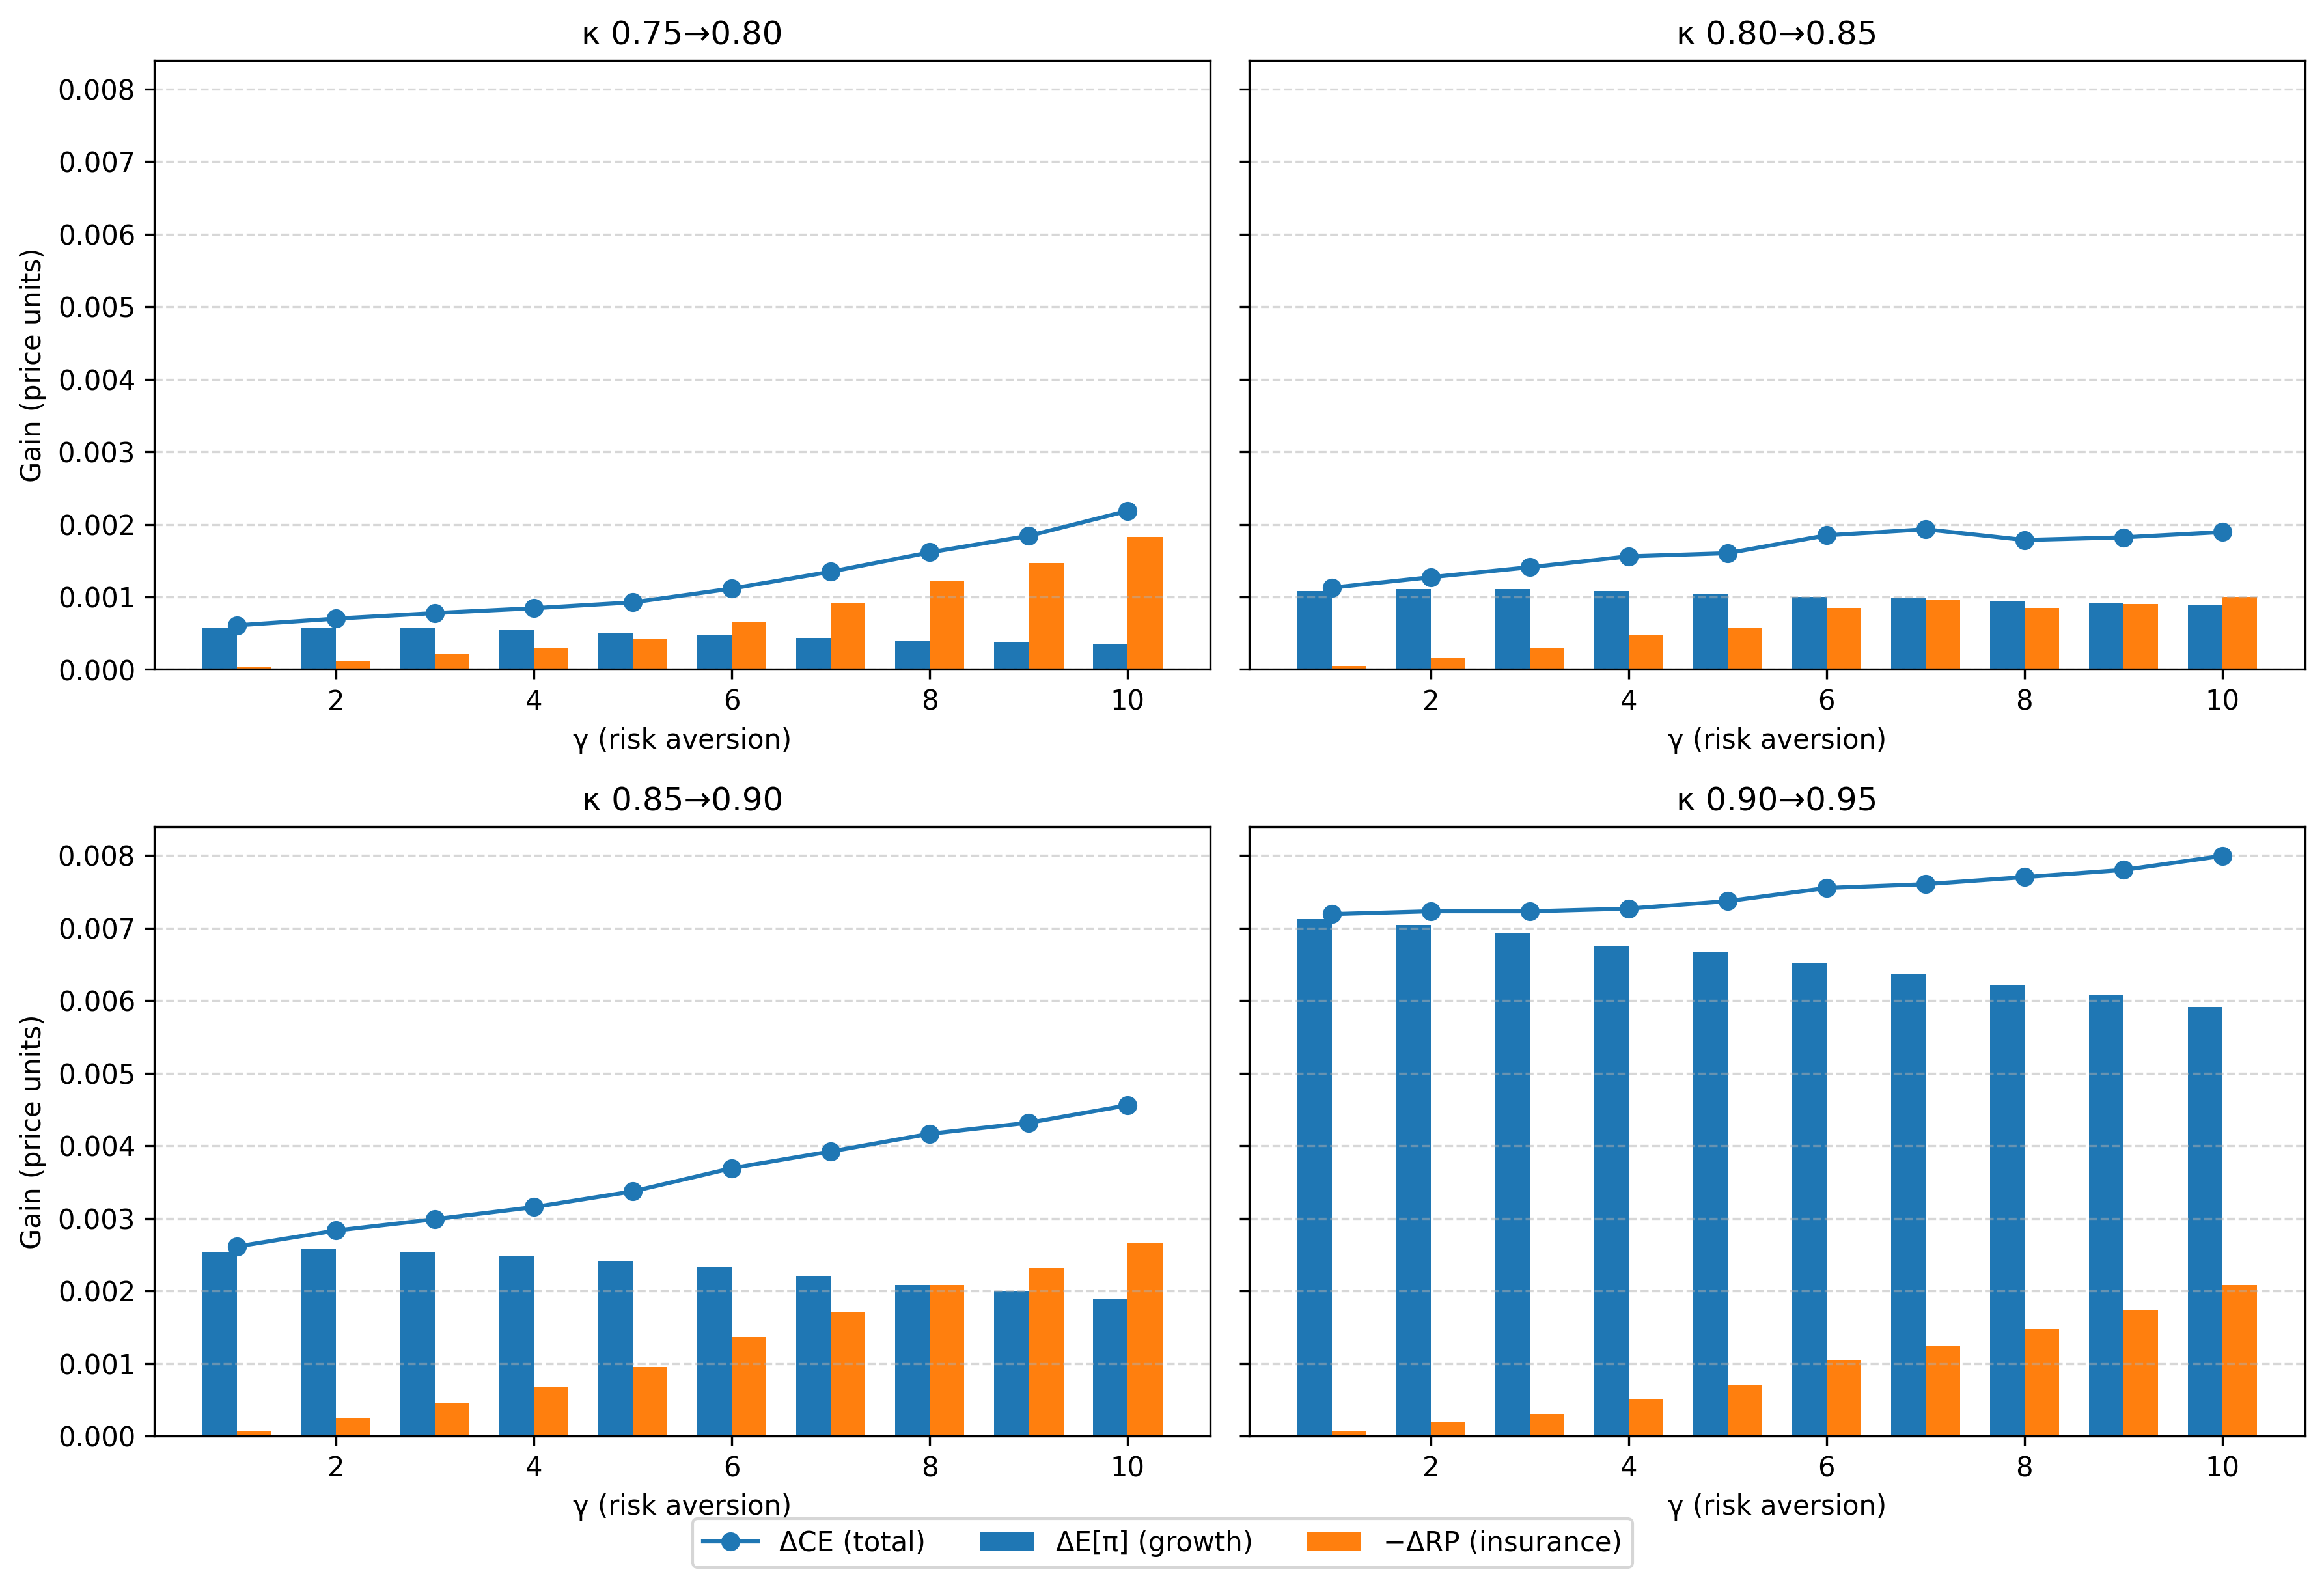
\includegraphics[width=\linewidth]{model_figures/storage_subsidy_gain_decomposition.png}
    \caption{Decomposition of Welfare Gains from Storage Subsidies by Risk Aversion}
    \label{fig:storage_subsidy_gain_decomposition}
    \begin{tablenotes}
    \footnotesize
    \item Note: Each panel reports results for one storage-efficiency contrast. For each buyer-power mean $\mu=\mu_1=\mu_2$, we simulate $R=5000$ worlds $(\theta_1,\theta_2)$ from Beta$(\mu,\sigma^2=0.10)$. Farmers ($N=100$) have heterogeneous risk preferences, with $\gamma \sim U[0,10]$ grouped into deciles. Bars show the decomposition of welfare gains into growth ($\Delta E[\pi]$) and insurance ($-\Delta RP$); the line shows the certainty-equivalent gain ($\Delta CE$). All values are averaged across $\mu \in [0.15,0.85]$ in steps of 0.05.
    \end{tablenotes}
\end{figure}

In Figure~\ref{fig:storage_subsidy_gain_decomposition}, each panel corresponds to one contrast in storage efficiency, $\kappa \in \{0.75\to0.80,\,0.80\to0.85,\,0.85\to0.90,\,0.90\to0.95\}$. For each buyer-power mean $\mu=\mu_1=\mu_2 \in [0.15,0.85]$ (in steps of 0.05), I simulate $R=5000$ worlds of $(\theta_1,\theta_2)$ from Beta distributions with variance $\sigma^2=0.10$. Farmers are heterogeneous in risk preferences, with $N=100$ draws of $\gamma \sim U[0,10]$ grouped into deciles, where the horizontal axis indexes $\gamma$-decile 1 (least risk-averse) through 10 (most risk-averse). Within each decile I plot: (i) a bar for the change in expected income, $\Delta E[\pi]$ (``income growth''), (ii) a bar for the insurance gain, $-\Delta RP$ (the reduction in risk premium, shown as a positive quantity), and (iii) a line for the certainty equivalent effect, $\Delta CE$. Reported values are averages across all $\mu$ scenarios.

The decomposition clarifies that the welfare effects of improving storage efficiency operate through two distinct channels---income growth and risk reduction. In most cases, $\Delta CE$ exceeds $\Delta E[\pi]$, implying $\Delta RP<0$: the improvement in storage technology reduces income variance and hence the risk premium. This arises because, for $\kappa<1$ and interior $s^\in(0,1)$, the income mix $(1-s^\star)p_1 + s^\star\kappa p_2$ has lower variance than the harvest-only benchmark, since $(1-s^\star)^2 + (s^\star\kappa)^2 < 1$. In other words, optimal storage functions as a state-contingent hedge: farmers store more in low-price states and less in high-price states, effectively truncating downside risk while tempering extreme upside realizations. Even when expected income gains are modest, the induced risk smoothing raises certainty-equivalent welfare.

When $\kappa$ is already relatively high, such as in the $0.90 \rightarrow 0.95$ contrast, the incremental welfare gains are larger than in the low-efficiency step $0.75 \rightarrow 0.80$. This convexity arises because higher storage efficiency strengthens both the intensive and extensive margins of storage. Farmers who were previously indifferent or weakly storing increase their storage share, while those already storing gain more from improved efficiency, so the aggregate response magnifies the value of each incremental subsidy.

At lower baseline levels of $\kappa$, the gains are smaller in absolute value but dominated by insurance effects, concentrated among more risk-averse deciles. In the $0.75 \rightarrow 0.80$ step, for example, the reduction in risk premium ($- \Delta RP$) is relatively more pronounced. These early-stage improvements thus act as insurance subsidies, offering the largest proportional benefits to farmers with high $\gamma$, for whom risk smoothing is most valuable. By contrast, once $\kappa$ reaches higher levels, additional subsidies reduce little risk and instead raise welfare almost exclusively through income growth. 

Taken together, the results from Figure~\ref{fig:storage_subsidy_gain_decomposition} highlight a dual policy message: early-stage investments in storage efficiency provide risk protection to vulnerable farmers, while later-stage improvements generate amplifying income effects by enabling more farmers to benefit from expanding market access and higher second-period competition. This heterogeneity underscores the importance of targeting and calibrating $\kappa$-enhancing interventions to local conditions rather than adopting a one-size-fits-all approach. 




\begin{figure}[ht]
    \centering
    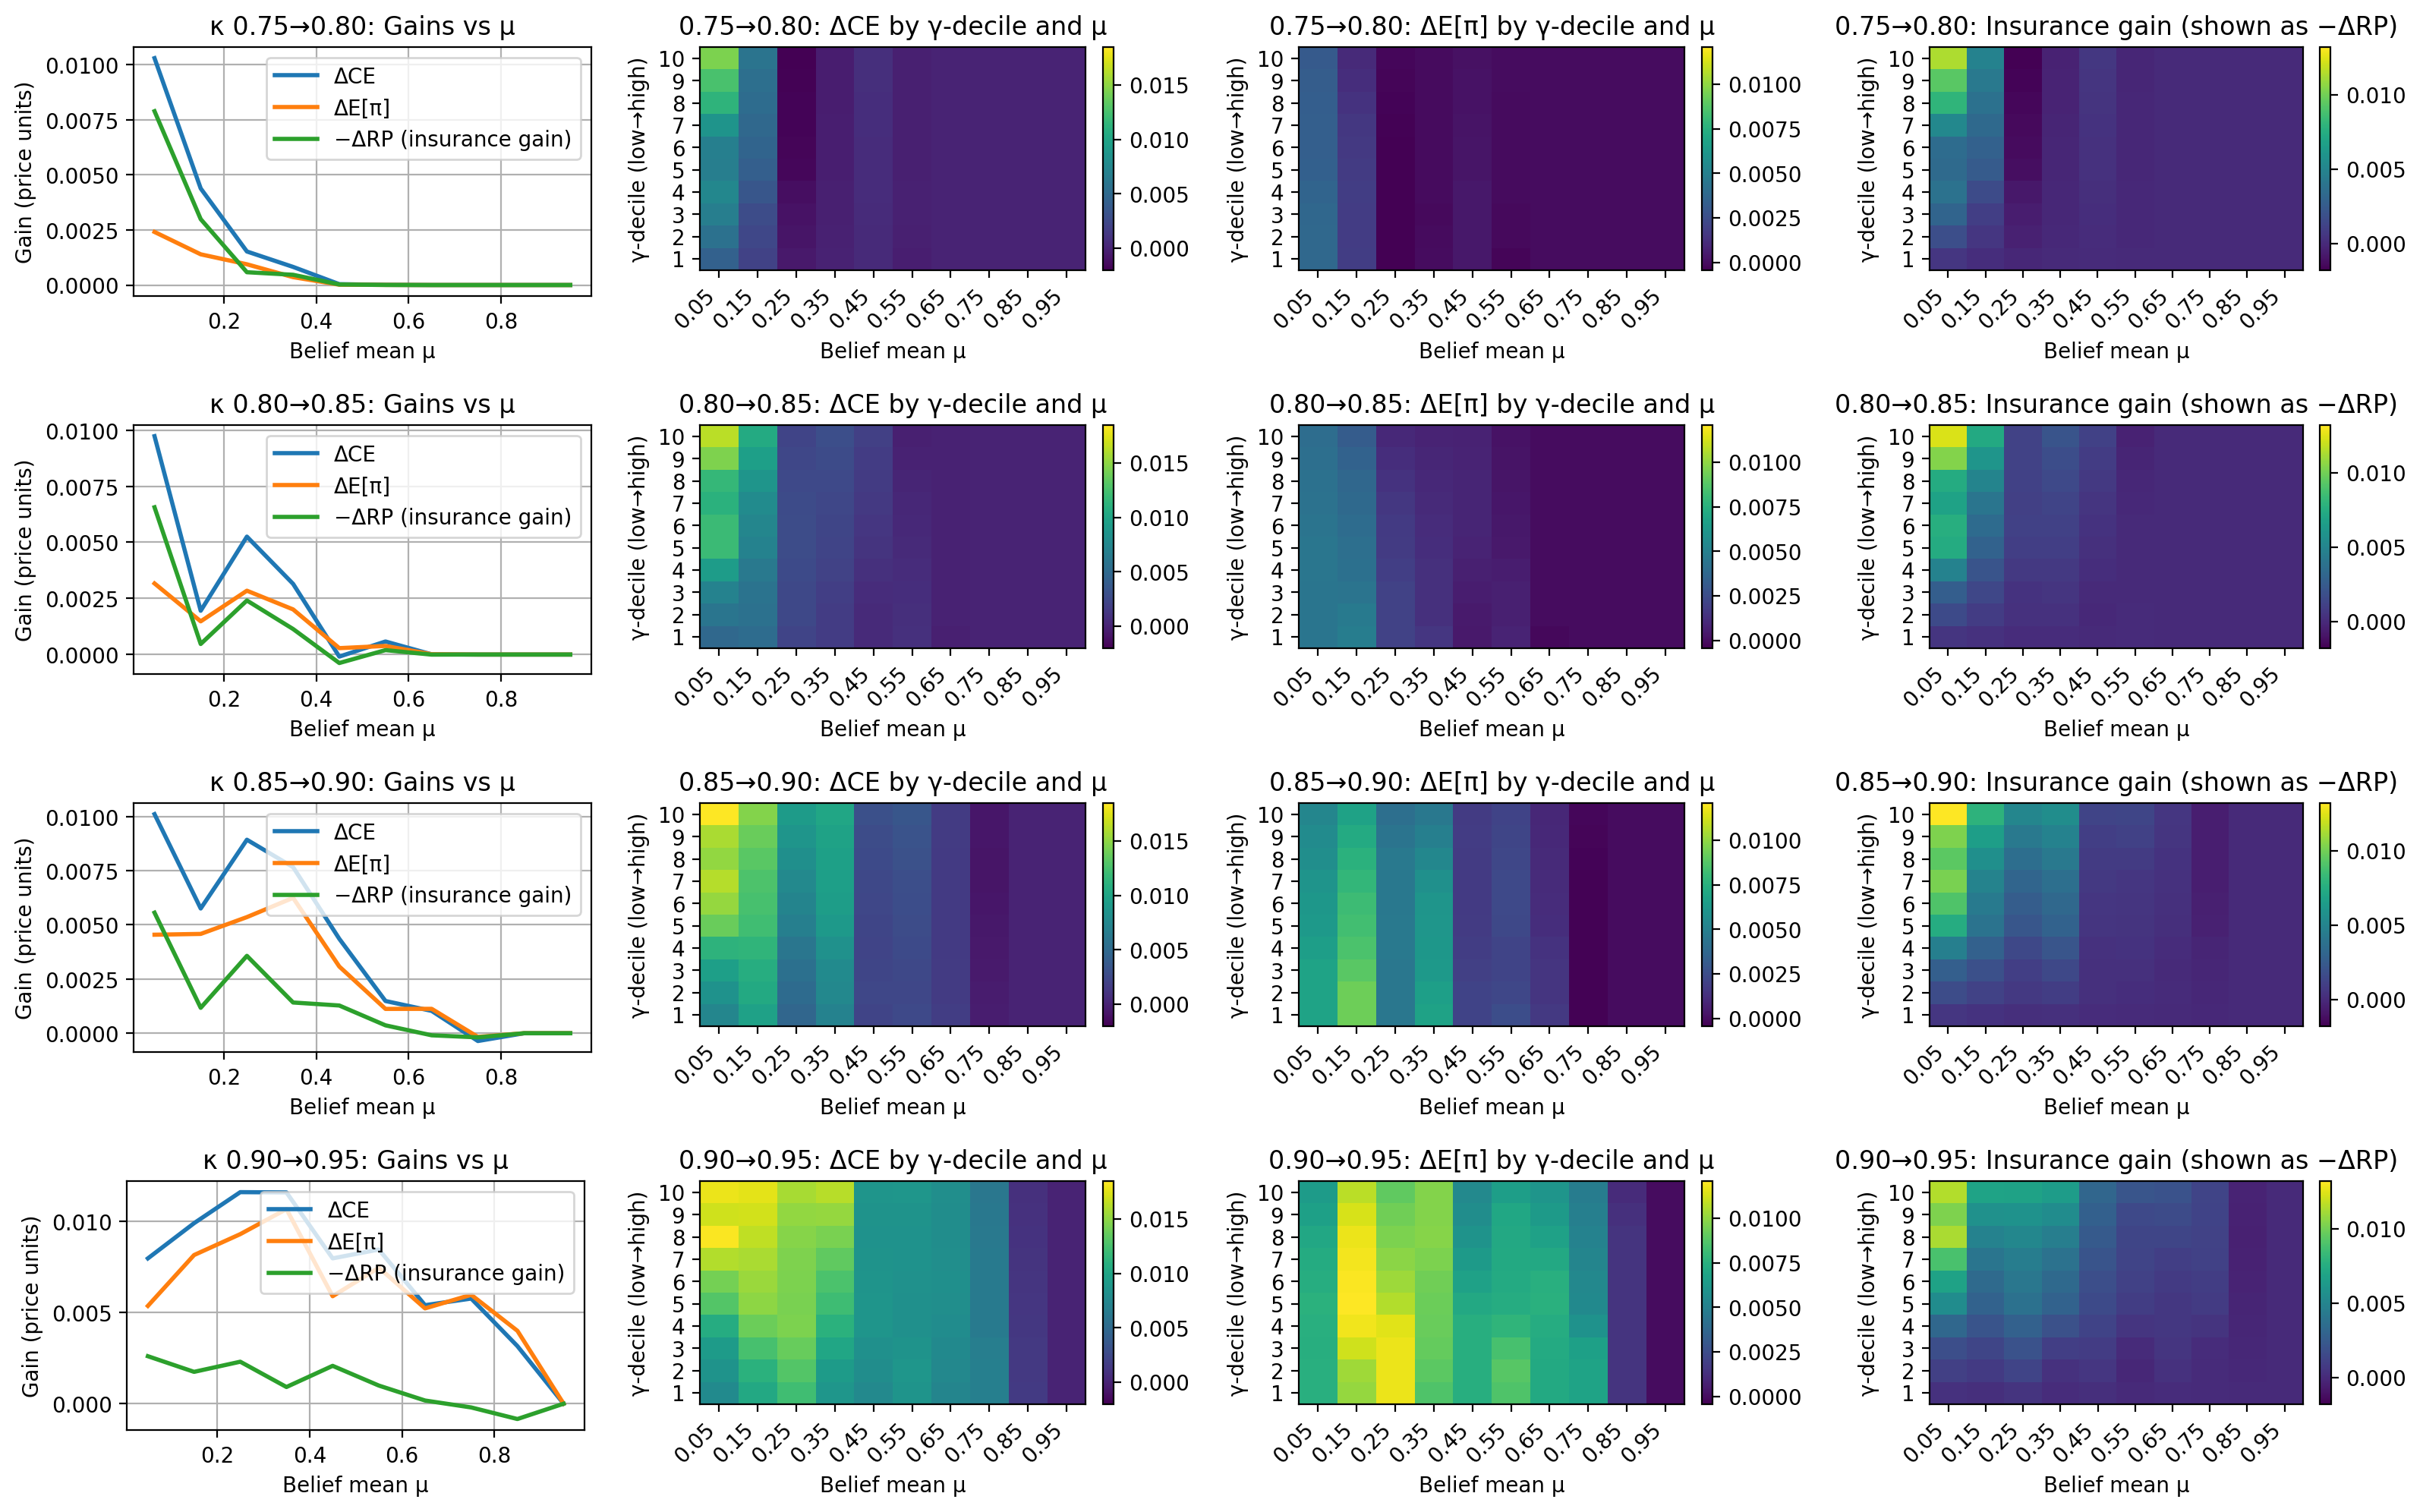
\includegraphics[width=\linewidth]{model_figures/storage_subsidy_gain_heatmap.png}
    \caption{Welfare Gains from Storage Subsidies: Line and Heatmap Decomposition across Buyer-Power Means and Risk Aversion}
    \label{fig: storage_subsidy_gain_heatmap}
    \begin{tablenotes}
    \footnotesize
    \item Note: Each row shows one subsidy contrast. Line charts (first column) plot changes in expected income ($\Delta E[\pi]$), certainty equivalent ($\Delta CE$), and insurance gain ($-\Delta RP$) against belief mean $\mu$. Heatmaps (columns 2--4) decompose these effects across $\gamma$-deciles, highlighting that welfare improvements are strongest for more risk-averse farmers and grow with the size of the subsidy.
    \end{tablenotes}
\end{figure}

To dig deeper, Figure~\ref{fig: storage_subsidy_gain_heatmap}, organized as a $4 \times 4$ panel, explores how welfare effects unfold across the full range of buyer-power means ($\mu$, x-axis), holding variance fixed at 0.10. Each row corresponds to one increment contrast, consistent with Figure~\ref{fig:storage_subsidy_gain_decomposition}. The first column presents line plots of the three welfare components (expected income, certainty equivalent, and insurance gain) while the remaining columns display heatmaps that further decompose these outcomes by risk-aversion deciles ($\gamma$, y-axis). Lighter colors in the heatmaps indicate stronger welfare improvements of per-unit storage-efficiency increment, underscoring how both mean buyer power across two periods and farmers' heterogeneity in risk preferences shape distributional effects.

The line plots reveal that when buyer power is weak (low $\mu$), income growth and certainty-equivalent gains remain similar across all increment contrasts, regardless of initial storage efficiency. In contrast, as buyer power strengthens, increments allocated to environments with higher baseline efficiency ($\kappa$) yield disproportionately larger welfare improvements. This pattern is evident in the flattening slopes of the income and CE curves as one moves down the rows of column one. In other words, the incremental aggregate welfare gains highlighted in Figure~\ref{fig:storage_subsidy_gain_decomposition} are driven primarily by the stronger performance of high-efficiency villages under high buyer power in both periods, rather than by differences at the lower end of the buyer-power distribution.


\paragraph{Policy lessons.}
Per-unit storage subsidies should be targeted to baseline conditions rather than deployed uniformly. At low initial storage efficiency (high ongoing storage costs), subsidies act chiefly as insurance---most valuable for high-$\gamma$ (more risk-averse) farmers---and should be paired with credit/guarantee or index-insurance instruments that lower effective risk aversion and crowd in participation. At high initial efficiency, the same-amount subsidy becomes a growth multiplier, with gains driven by higher mean returns rather than risk reduction; dollars spent here yield larger aggregate welfare per unit outlay, especially where $\sigma^2$ is meaningful. A practical design is a tiered schedule: insurance-oriented support for low-$\kappa$ environments (with eligibility keyed to observable storage losses) and performance-linked, sunset-eligible subsidies for high-$\kappa$ areas, complemented by measures that reduce $\gamma$ (credit/insurance) and by competition policies.


%----------------------------------------------------%
\subsection{Welfare Effects of Lower Farmer Risk Aversion}
\noindent Beyond storage subsidies, the aggregate welfare value of intertemporal storage depends critically on farmer risk preferences. Risk attitudes are partly innate, but they are also mediated by financial frictions: wealthier households typically exhibit lower effective risk aversion, and improved access to credit or insurance reduces the degree of prudence applied to marketing decisions.

This subsection evaluates how lower risk aversion enhances the value of storage when second-period buyer power mirrors the first. Figure~\ref{fig: Income gains with RN case} reports village-average income gains from storage relative to the no-storage benchmark by heterogeneous risk aversion. The figure adopts the same $4\times4$ structure as Figure~\ref{fig: Income gains}, with rows varying storage efficiency $\kappa$ and columns varying the variance of buyer power $\sigma^2$. Within each panel, the horizontal axis shows the common mean buyer power, $\mu=\mu_1=\mu_2$. Three curves contrast alternative risk environments of our 100-farmer village: (i) the risk-neutral envelope ($\gamma=0$), (ii) moderately risk-averse farmers ($\gamma_i\sim \mathrm{Unif}[0,5]$), and (iii) more risk-averse farmers ($\gamma_i\sim \mathrm{Unif}[0,10]$). The vertical gap between the risk-neutral line and heterogeneous curves quantifies the income foregone due to prudence.

\begin{figure}[ht]
    \centering
    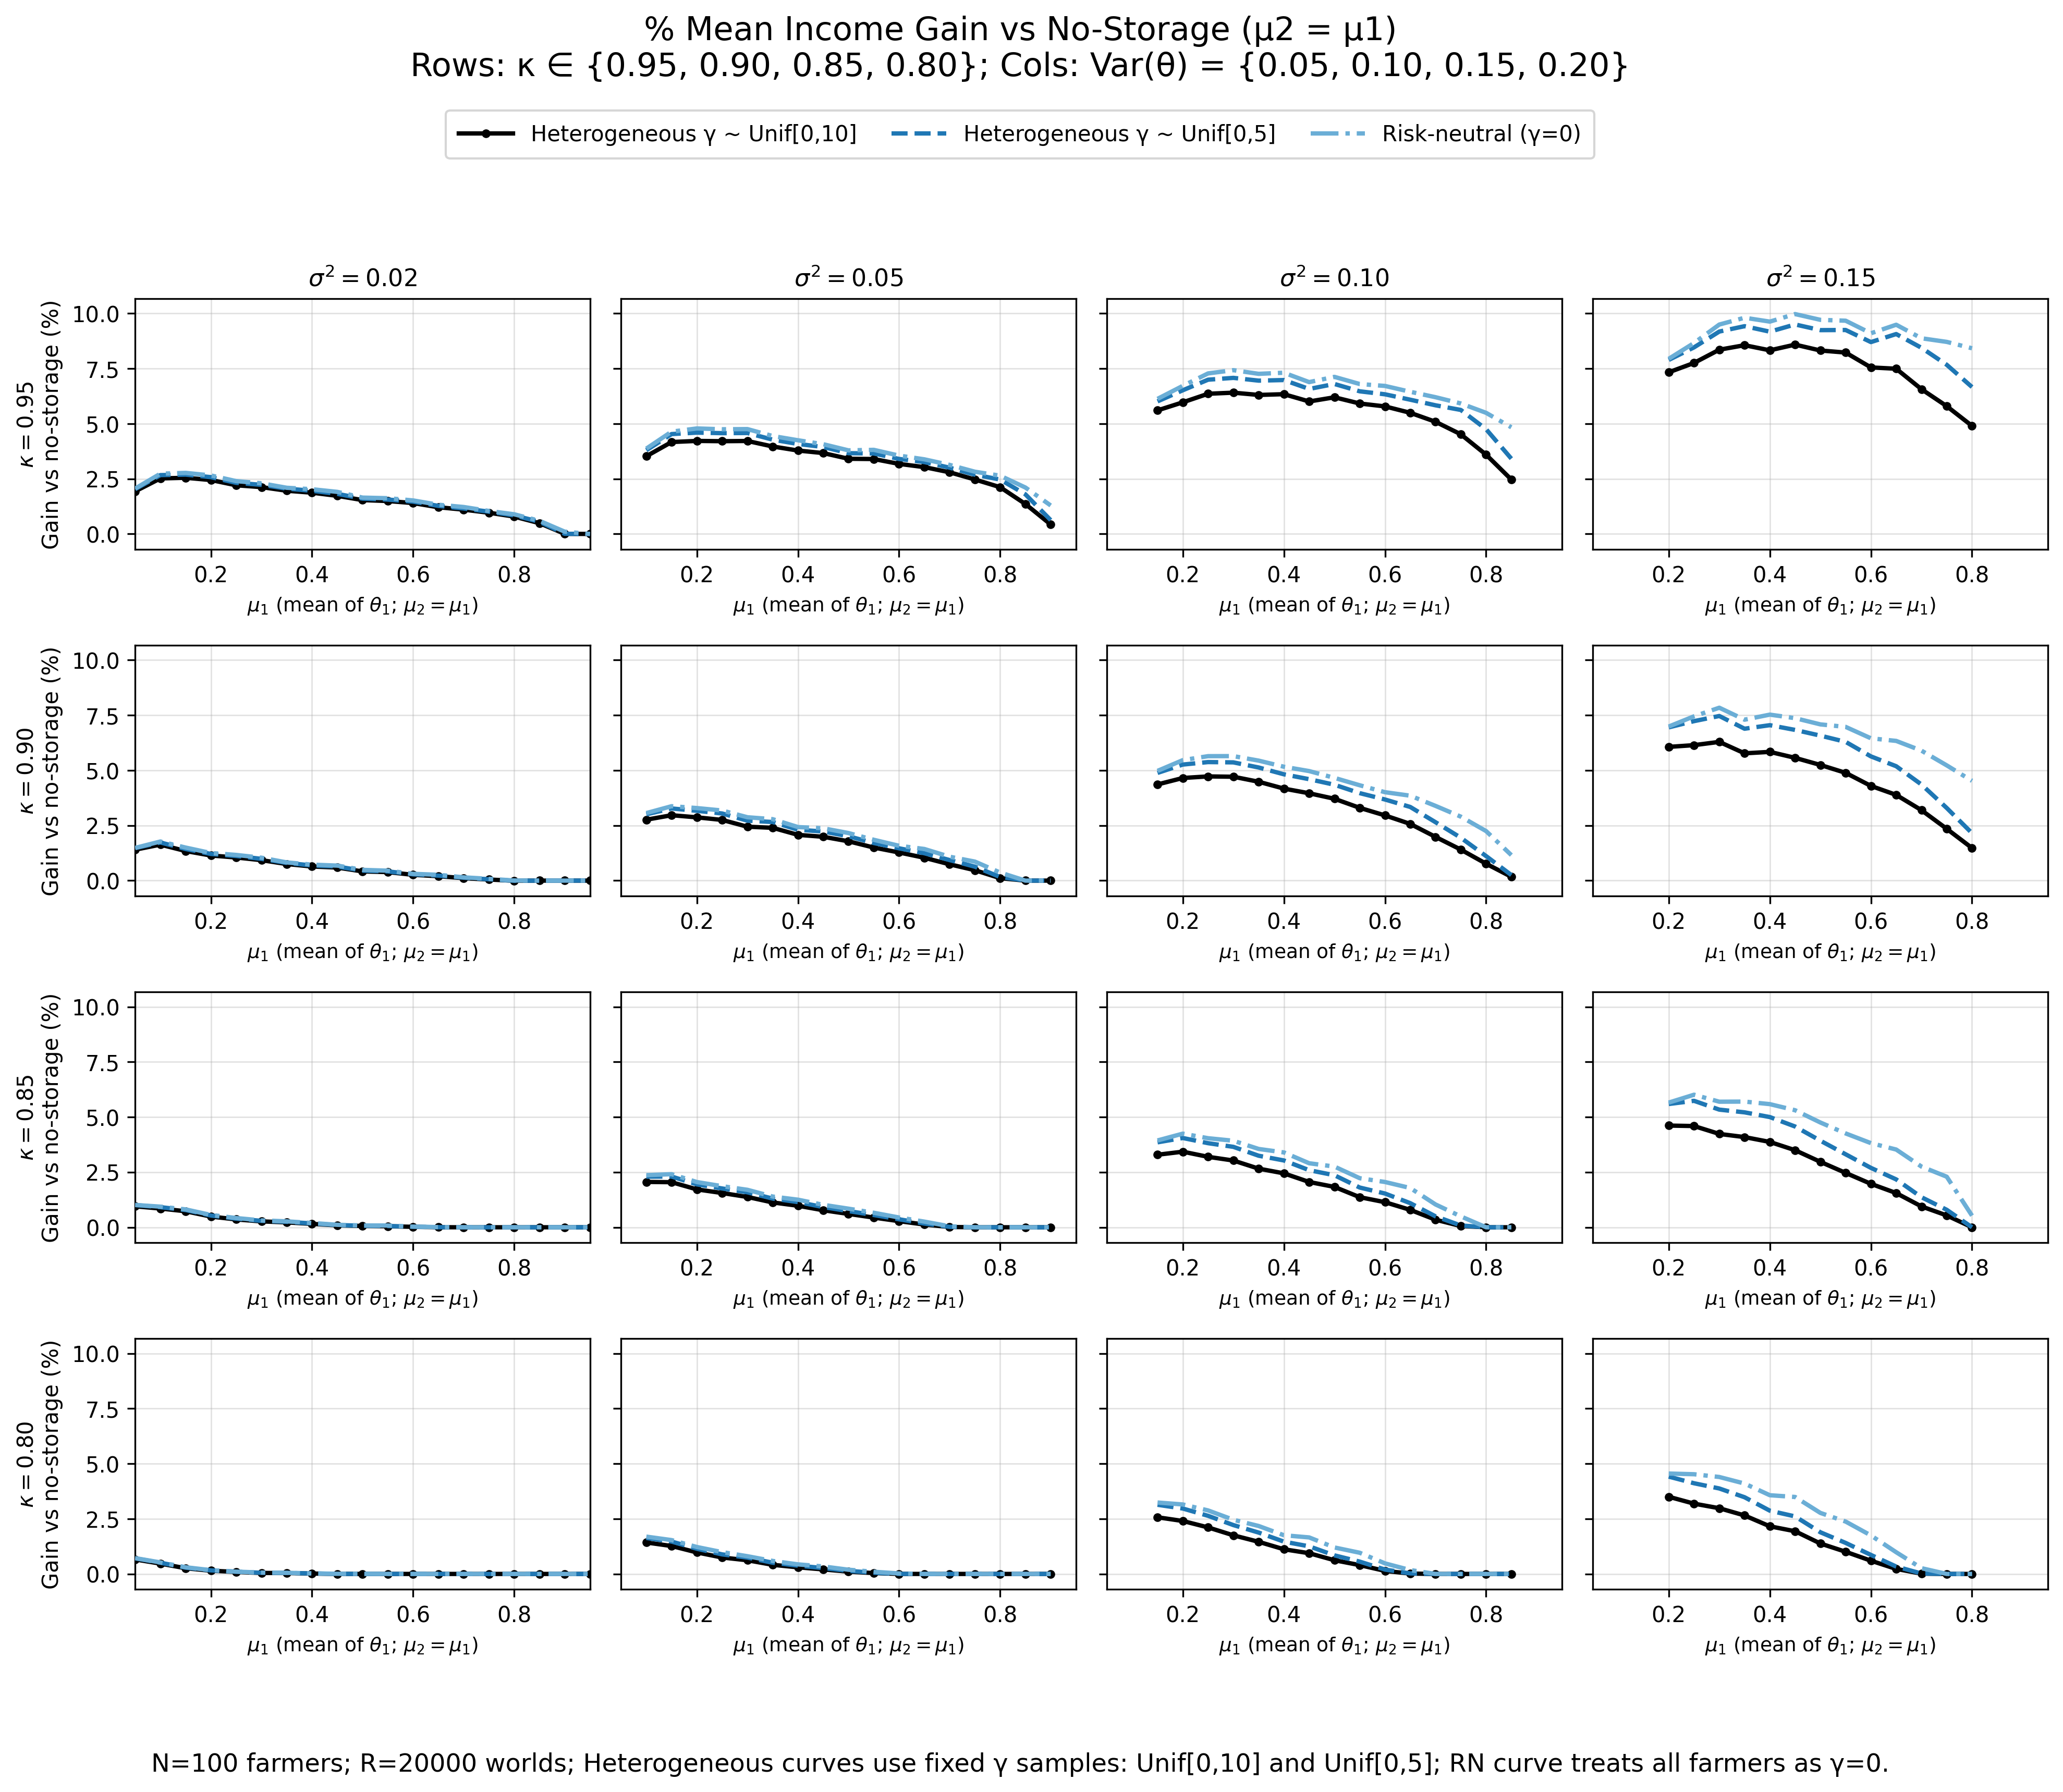
\includegraphics[width=\linewidth]{model_figures/gainpct_grid_4x4_zero_gap_three_curves.png}
    \caption{$\%$ Mean Income Gains under High, Median, and No Risk Aversion}
    \label{fig: Income gains with RN case}
    \begin{tablenotes}
    \footnotesize
    \item Note: Panels show mean income gains from storage relative to no-storage under the zero-gap case ($\mu_2=\mu_1$). Rows vary storage efficiency and columns vary buyer-power variance. Curves compare heterogeneous farmers with $\gamma_i \sim \text{Unif}[0,10]$ (black solid) and $\gamma_i \sim \text{Unif}[0,5]$ (blue dashed) against the risk-neutral benchmark ($\gamma=0$, light-blue dash-dotted). Results average $R=20{,}000$ simulated worlds with $N=100$ farmers each.
    \end{tablenotes}
\end{figure}

Lower risk aversion systematically shifts the heterogeneous-$\gamma$ curves upward toward the risk-neutral envelope. Under higher buyer-power variance (right-hand columns), reducing village risk aversion yields additional income gains on the order of 1-5 percentage points, with the largest improvements realized when $\kappa$ is high and $\mu$ is interior (neither too close to 0 nor 1). By contrast, in low-return settings (bottom-left panels with low $\kappa$ and low $\sigma^2$), all curves converge near the axis at low $\mu$, and differences across risk profiles are economically negligible.

Two comparative statics emerge cleanly. First, holding $\sigma^2$ fixed, the divergence between risk-neutral and heterogeneous-$\gamma$ outcomes is increasing in $\kappa$. Greater storage efficiency magnifies the upside to reallocating revenue inter-temporally; risk-neutral farmers exploit this fully, whereas more risk-averse farmers shade down optimal storage $s^*$, leaving gains unrealized. Second, holding $\kappa$ fixed, the wedge is increasing in $\sigma^2$. Volatility raises the value of timing but also the exposure to downside realizations; prudence truncates this upside more aggressively when $\gamma$ is larger. Together, higher $\kappa$ and higher $\sigma^2$ amplify the stakes of the storage decision and widen the gap between cautious and risk-neutral behavior.


\paragraph{Policy lessons.} 
Interventions that effectively reduce $\gamma$ (for example, affordable short-term credit lines collateralized by inventories, partial revenue insurance contingent on ex-post prices, or group-based risk pooling) translate into measurable income gains in environments with sufficiently high $\kappa$ and/or $\sigma^2$. Where $\kappa$ is very low and price risk muted, altering $\gamma$ has little bite; lowering storage costs (raising $\kappa$) is then the first-order lever. Conversely, in high-$\kappa$, high-$\sigma^2$ markets, even modest reductions in effective risk aversion close much of the welfare gap relative to the risk-neutral frontier.




\begin{table}[ht!]\centering
\caption{Simulated Storage Outcomes with Equal Mean Buyer Power}
\label{tab:mu_cases_storage_outcomes}
\begin{threeparttable}
\vspace{0.35em}
\noindent\textbf{Panel A. Expected Income Gain vs No Storage (\%)}
\vspace{0.25em}
\begin{tabular}{l|ccc|ccc|ccc}
\toprule
 & \multicolumn{3}{c|}{$\mu=0.2$} & \multicolumn{3}{c|}{$\mu=0.5$} & \multicolumn{3}{c}{$\mu=0.8$} \\
Var($\theta$) & $\kappa=0.80$ & $\kappa=0.90$ & $\kappa=0.95$ & $\kappa=0.80$ & $\kappa=0.90$ & $\kappa=0.95$ & $\kappa=0.80$ & $\kappa=0.90$ & $\kappa=0.95$ \\
\midrule
0.02 & 0.16 & 1.22 & 2.42 & 0.00 & 0.47 & 1.61 & 0.00 & 0.00 & 0.79 \\
0.05 & 0.99 & 2.89 & 4.32 & 0.09 & 1.71 & 3.53 & 0.00 & 0.05 & 1.88 \\
0.10 & 2.36 & 4.62 & 6.01 & 0.61 & 3.61 & 6.01 & 0.00 & 0.72 & 3.66 \\
0.15 & 3.60 & 5.87 & 7.26 & 1.45 & 5.34 & 8.35 & 0.00 & 1.59 & 5.15 \\
\bottomrule
\end{tabular}

\vspace{0.35em}
\noindent\textbf{Panel B. Certainty Equivalent Gain vs No Storage (\%)}
\vspace{0.25em}
\begin{tabular}{l|ccc|ccc|ccc}
\toprule
 & \multicolumn{3}{c|}{$\mu=0.2$} & \multicolumn{3}{c|}{$\mu=0.5$} & \multicolumn{3}{c}{$\mu=0.8$} \\
Var($\theta$) & $\kappa=0.80$ & $\kappa=0.90$ & $\kappa=0.95$ & $\kappa=0.80$ & $\kappa=0.90$ & $\kappa=0.95$ & $\kappa=0.80$ & $\kappa=0.90$ & $\kappa=0.95$ \\
\midrule
0.02 & 0.39 & 2.10 & 3.62 & 0.00 & 0.60 & 1.90 & 0.00 & 0.00 & 0.71 \\
0.05 & 2.45 & 5.80 & 7.90 & 0.12 & 2.09 & 4.20 & 0.00 & 0.01 & 1.40 \\
0.10 & 5.72 & 10.19 & 12.67 & 0.70 & 4.17 & 6.89 & 0.00 & 0.49 & 2.50 \\
0.15 & 8.59 & 13.43 & 15.99 & 1.65 & 6.04 & 9.10 & 0.00 & 1.18 & 3.42 \\
\bottomrule
\end{tabular}

\vspace{0.35em}
\noindent\textbf{Panel C. Mean Storage Share}
\vspace{0.25em}
\begin{tabular}{l|ccc|ccc|ccc}
\toprule
 & \multicolumn{3}{c|}{$\mu=0.2$} & \multicolumn{3}{c|}{$\mu=0.5$} & \multicolumn{3}{c}{$\mu=0.8$} \\
Var($\theta$) & $\kappa=0.80$ & $\kappa=0.90$ & $\kappa=0.95$ & $\kappa=0.80$ & $\kappa=0.90$ & $\kappa=0.95$ & $\kappa=0.80$ & $\kappa=0.90$ & $\kappa=0.95$ \\
\midrule
0.02 & 0.03 & 0.15 & 0.25 & 0.00 & 0.11 & 0.26 & 0.00 & 0.01 & 0.26 \\
0.05 & 0.10 & 0.19 & 0.25 & 0.03 & 0.21 & 0.33 & 0.00 & 0.09 & 0.39 \\
0.10 & 0.14 & 0.20 & 0.22 & 0.11 & 0.28 & 0.37 & 0.00 & 0.20 & 0.44 \\
0.15 & 0.16 & 0.18 & 0.19 & 0.17 & 0.32 & 0.39 & 0.00 & 0.25 & 0.46 \\
\bottomrule
\end{tabular}

\vspace{0.35em}
\noindent\textbf{Panel D. Share of Storage Adopters}
\vspace{0.25em}
\begin{tabular}{l|ccc|ccc|ccc}
\toprule
 & \multicolumn{3}{c|}{$\mu=0.2$} & \multicolumn{3}{c|}{$\mu=0.5$} & \multicolumn{3}{c}{$\mu=0.8$} \\
Var($\theta$) & $\kappa=0.80$ & $\kappa=0.90$ & $\kappa=0.95$ & $\kappa=0.80$ & $\kappa=0.90$ & $\kappa=0.95$ & $\kappa=0.80$ & $\kappa=0.90$ & $\kappa=0.95$ \\
\midrule
0.02 & 0.05 & 0.23 & 0.34 & 0.00 & 0.16 & 0.35 & 0.00 & 0.06 & 0.35 \\
0.05 & 0.16 & 0.27 & 0.36 & 0.08 & 0.32 & 0.45 & 0.00 & 0.35 & 0.55 \\
0.10 & 0.21 & 0.26 & 0.30 & 0.26 & 0.42 & 0.50 & 0.00 & 0.64 & 0.71 \\
0.15 & 0.21 & 0.21 & 0.22 & 0.38 & 0.48 & 0.51 & 0.00 & 0.78 & 0.79 \\
\bottomrule
\end{tabular}
\
\begin{tablenotes}[flushleft]
\footnotesize
\item Notes: $N=100$, $R=20000$, $\gamma\sim U[0,10]$. Prices $p=1/(1+\theta)$. $\theta_1,\theta_2\sim \text{Beta}(\alpha,\beta)$ calibrated to $(\mu,\sigma^2)$. Policy $s^*(\theta_1,\gamma)$ solved by golden-section; expectation over $\theta_2$ by 12-point Gauss-Legendre quadrature. Adopters: $s^*>0.01$.
\end{tablenotes}
\end{threeparttable}
\end{table}



\subsection{Numerical Outcomes under Identical Buyer Power Distributions}
\noindent The preceding visualizations discover the relationships between storage efficiency, buyer power, and welfare outcomes. Table~\ref{tab:mu_cases_storage_outcomes} complements those insights by providing direct estimates for a non-favorable case in which buyer power in both periods is drawn from the same distribution, $\mu_1=\mu_2 \in {0.2,0.5,0.8}$. Even under this relatively restrictive environment, where intertemporal arbitrage opportunities are limited to variance rather than shifts in the mean, the positive role of storage for farmers is evident across welfare metrics. The observed patterns below are consistent with an option-value logic: storage delivers little when volatility is low or efficiency costs are high, but once either volatility or efficiency crosses a threshold, both adoption and welfare gains rise sharply.

In terms of expected income (Panel~A), storage is most valuable when buyer power is low and moderate ($\mu=0.2,0.5$). Here, gains generally climb with volatility and with efficiency, reaching 7--8\% at high $\kappa$ and Var($\theta$). By contrast, when buyer power is severe on average ($\mu=0.8$), storage rarely pays unless efficiency is very high; many cells yield essentially zero. This shows that timing value cannot offset uniformly depressed price environments.

Risk preferences alter this picture. The certainty-equivalent results in Panel~B show that storage is especially attractive to risk-averse farmers when average prices are reasonable ($\mu=0.2$). There, CE gains substantially exceed mean-income gains---up to 16\% versus 7\%---reflecting the insurance role of storage. Where market power is stronger ($\mu=0.8$), the insurance premium vanishes. The intermediate case ($\mu=0.5$) sits between these poles, with CE gains only modestly above expected income.

Panels~C and D distinguish the intensive and extensive margins of storage adoption. The share of adopters responds strongly to volatility and efficiency---at high $\mu$, participation jumps from near zero at low volatility to nearly 80\% at Var($\theta$)=0.15. Yet the mean storage share rises much more modestly. Many farmers adopt but store only a small portion, using storage as a contingent hedge rather than a bulk strategy. Where prices are favorable, higher volatility even reduces average storage shares, as farmers reallocate more selectively across states. This underscores that welfare gains are driven less by volume stored and more by the flexibility to reallocate at the margin.

Overall, the evidence here points to three additional findings. First, storage pays most where efficiency is high and buyer power is not overwhelming. Second, risk aversion amplifies the value of storage when price levels are healthy but dampens it when average prices are low. Third, adoption is sometimes broad but shallow---many farmers engage, but the welfare effect stems from precise timing rather than large shifts in volume. These results highlight that policy instruments which improve storage efficiency or help farmers bear the fixed costs of adoption will generate the largest welfare returns where volatility is substantial and average buyer power is not too extreme.


%----------------------------------------------------%
%----------------------------------------------------%


\section{Further Extensions}

\subsection{Other Models of Risk Preference}
\noindent According to \cite{o2018modeling}, ``Real-world risk aversion is clearly not as straightforward as expected utility suggests. Additional sources of risk aversion (or risk-seeking) need to be used instead of, or in conjunction with, diminishing marginal utility of wealth.'' Individuals assess options involving both gains and losses, the ``kink'' in the value function between losses and gains induces risk aversion. Therefore, future researchers may extend my model by exploring the Loss Aversion models \citep{kahneman1979prospect}, in addition to the expected utility theorem. The approach developed by \cite{kHoszegi2006model, kHoszegi2007reference, kHoszegi2009reference} in addressing loss aversion with an endogenous reference point aims to mitigate this degree of freedom by asserting that the reference point is entirely determined by one's expectations about outcomes. Empirical work also highlights the relevance of these alternative frameworks: for instance, \cite{liu2013risk} show that Chinese Bt cotton farmers' pesticide use is systematically related to their risk and loss aversion, with more risk-averse farmers applying greater quantities of pesticides and more loss-averse farmers applying less. Despite this evidence, there has been limited progress in adapting alternative models to dynamic settings, with a notable exception of \cite{kHoszegi2009reference}, who define loss aversion concerning changes in beliefs regarding both current and future consumption.



\subsection{Collective-Action Dilemma: The Storage ``Treadmill''}
\noindent Field observations suggest a collective-action dilemma surrounding storage adoption. As more farmers in a village adopt storage, middlemen may redirect procurement efforts to neighboring villages with less storage penetration, where farmers face weaker bargaining positions. This strategic shift reduces buyer competition at harvest in the original village, particularly disadvantaging farmers without storage. Consequently, farmers who have not adopted storage face mounting pressure to invest, not necessarily for higher profits, but to avoid worsening terms of trade. 

This dynamic mirrors the classic ``technology treadmill'' described by Cochrane \citep{cochrane1958farm, levins1996treadmill}. It describes how technological progress in agriculture often fails to generate lasting gains for farmers. Early adopters of a new technology temporarily benefit from lower costs and higher profits, but as adoption spreads, aggregate supply expands and output prices fall due to the inelastic demand for food. These price declines erode the initial advantages, leaving non-adopters increasingly disadvantaged and eventually compelling them to adopt merely to maintain their previous income levels. In this way, technology adoption becomes a defensive necessity rather than a source of sustained profit. Future extensions of the model could incorporate this endogenous spillover, possibly via a parameter capturing buyer response to aggregate storage rates, highlighting how individually rational behavior may generate suboptimal collective outcomes.






\subsection{Non-linear Storage Cost}
\noindent Storage costs for farmers, defined as the sum of the actual cost of renting or operating storage space and the cost of deterioration, could be non-linear in many cases. For perishable goods like apples, the primary reason for convex storage costs is probably that spoilage and quality deterioration increase over time. Also, the operating costs of storage may not increase linearly with the volume of goods stored. Managing temperature and humidity conditions for larger quantities might require more sophisticated technology and energy consumption, leading to non-linear cost increases.

Supporting this notion, \cite{williams1989economic} demonstrates, through a quadratic form of total marketing costs, that farmers need to weigh the marginal revenue of later sales against the elevated costs incurred. This balance leads to a positive inventory, even without considering risk aversion. Instead of capturing the composite storage cost by a discounting factor, a well-designed mathematical model would allow other forms of storage costs, therefore, may give us other relevant real-world policy implications.


\section{Conclusion}
\noindent This chapter develops a conceptual framework to analyze farmers' storage behavior under buyer market power. Storage adoption creates an inter-temporal arbitrage margin that allows farmers to shift sales across periods, thereby mitigating the effects of oligopsony at harvest and enhancing their bargaining position. The model shows that even absent shifts in aggregate demand or supply, temporal variation in buyer competition alone can make storage a valuable marketing tool.

The model provides a theoretical basis for small-scale farmers' storage and marketing choices. It focuses on farmers' intra-seasonal strategies and the storing-decision process, where farmers observe farm-gate prices and market structure at harvest and decide whether to immediately sell some, all, or none of their crops. When farmers have insufficient bargaining power at a single point in time, the adoption of storage at lower storage costs would give them inter-temporal arbitrage opportunities.

Although motivated by the fresh-apple industry, the model's logic applies broadly across perishable commodities. Storage and inventory play a central role in agricultural marketing systems, not only smoothing demand-driven price fluctuations but also reshaping the strategic interaction between growers and buyers. Framing storage as a tool to navigate imperfect competition thus extends beyond post-harvest logistics to the core of market efficiency and farmer welfare.

Policy implications follow directly from the analysis. First, lowering storage costs through subsidies, credit, or investment in modern facilities expands the set of circumstances under which farmers can profitably store and arbitrage across periods. Second, strengthening competition among buyers, via enforcement of antitrust rules, lower entry barriers for new buyers, or improved transparency in local markets, raises the effective price level and reduces the rents extracted by middlemen. Third, reducing the effective bite of risk aversion, through crop insurance, safety nets, or access to seasonal finance, encourages farmers to undertake storage when it is profitable in expectation but risky. Together these instruments highlight a policy strategy that does not rely on direct price support or costly procurement programs, but instead empowers farmers to use inter-temporal arbitrage to raise incomes and improve efficiency along the supply chain.






% %---------------------------%
% \newpage
% \section{Memo: A Difficult Tradeoff between Two Utility Aggregation Approaches}
% \noindent As I finalize revisions on the current model, I identify a major conceptual drawback: the optimal storage share becomes increasing in the farmer's degree of risk aversion when the expected second-period buyer power is higher than the first-period level. In other words, the model implies that farmers who expect a worse market condition in the future would store more if they are more risk-averse. This result is counterintuitive and lacks a clear behavioral or economic justification.

% This inconsistency has prompted me to revisit an alternative formulation we previously considered. Specifically, we face a fundamental modeling choice between:
% \begin{itemize}
%     \item Maximizing the expected sum of discounted utilities of income, versus
%     \item Maximizing the utility of the sum of discounted incomes.
% \end{itemize}
% Both approaches are theoretically sound but carry distinct implications. Below, I outline the tradeoffs between the two so we can more clearly evaluate the direction forward.

% \subsection{Current Setting: Sum of Discounted Utilities of Income}

% \noindent This is the standard formulation in intertemporal utility theory, where utility is evaluated separately in each period and future utility is discounted by a factor $\delta$:
% \begin{equation}
% \max_{s \in [0,1]} ; U\left((1 - s) p_1\right) + \delta \cdot \mathbb{E} \left[ U\left(s \cdot p_{2,\text{net}} \right) \right].
% \end{equation}

% \noindent Key assumptions and implications:
% \begin{itemize}
% \item Utility is additive and separable across time.
% \item The agent is risk-averse within each period, but not across periods.
% \item This structure implies a preference for income smoothing over time.
% \end{itemize}

% The primary advantage of this formulation lies in its analytical tractability. The separability allows us to derive a closed-form solution for the optimal storage share $s^*$, even under nontrivial distributional assumptions about future buyer power. It fits neatly within the expected utility framework and supports comparative statics analysis with intuitive results, except for the key case of higher second-period buyer power involving risk aversion.

% Through simulation and sensitivity checks (see Figure), I observe a troubling result: when expected second-period buyer power is pessimistic ($\theta_2$ is larger), the optimal storage share becomes increasing in risk aversion. This is counterintuitive. Typically, greater risk aversion should lead agents to reduce exposure to future uncertainty--i.e., store less. This expected behavior holds in the left region of the figure (where expectations about the future are optimistic), but breaks down in the right region.

% Upon closer inspection, this anomaly stems from the fact that the model assumes risk aversion only within periods. The framework lacks intertemporal risk aversion--i.e., there is no mechanism to penalize uncertainty in total income across periods. Unless we fundamentally alter the utility function (e.g., by adopting a non-additive or piecewise utility structure), this counterintuitive outcome cannot be avoided within this setting.

% One might ask how prior literature addresses this. The answer is: they often avoid it by making restrictive assumptions or narrowing the scope of analysis. For instance, \citet{ruhinduka2020smallholder} (the work by Travis Lybbert and his co-authors studying the post-harvest storage decisions) assume $\mathbb{E}(p_2) > p_1$, ensuring that $\partial s^* / \partial \gamma < 0$, thus sidestepping the unintuitive regime altogether.


% \subsection{Alternative Setting: Utility of the Sum of Discounted Income}
% \noindent This alternative formulation, similar to the structure used in your work with Saitone and Malan \citep{saitone2018price}, applies the utility function to the entire stream of income, aggregated and discounted to the present:
% \begin{equation}
% \max_{s \in [0,1]} ;\mathbb{E} \left(U\left[ (1 - s) p_1 + \delta \cdot s \cdot p_{2,\text{net}} \right]\right).
% \end{equation}

% \noindent Key assumptions and implications:
% \begin{itemize}
% \item Utility is applied to the total discounted income as a single aggregated payoff.
% \item The agent exhibits intertemporal risk aversion--preferences depend on risk in the total income stream, not just within each period.
% \item This formulation is commonly used in investment and project evaluation models, especially under uncertainty.
% \end{itemize}

% The primary strength of this setting is its consistency with empirical observations. Simulations under a CRRA utility specification (see Figure show that both risk-neutral and most moderately risk-averse farmers tend to make corner solutions--either storing everything or nothing--which aligns well with real-world behavior. Interior solutions exist but are confined to a narrow region of the parameter space, unlike the smoother, wider range of partial storage outcomes generated by the standard model.

% The main limitation, however, is analytical intractability. Closed-form solutions for the optimal storage share $s^*$ are not available under arbitrary distributions of $\theta_2$ in our case. Solving this model typically requires numerical methods, which restrict our ability to conduct formal comparative statics. An exception arises in cases with a finite number of discrete scenarios--e.g., buyer competition modeled as Bertrand duopoly with known probabilities--in which case closed-form solutions may be derived. Otherwise, we must rely on simulation-based approximation.

% \subsection{3D Visualizations of Both Formulations}

% \noindent I conduct simulations for both utility formulations over a grid defined by the coefficient of relative risk aversion ($\gamma$) and the storage efficiency factor ($\kappa$). The first-period buyer power is fixed at $\theta_1 = 0.6$, and the discount factor is set at $\delta = 1.0$ throughout.

% Figure~\ref{fig:3D_formulation} presents a $4 \times 4$ panel summarizing the simulation results. I examine eight distinct Beta distributions for $\theta_2$, varying in both the mean and variance: two levels of variance--low ($\sigma^2 = 0.02$) and high ($\sigma^2 = 0.05$)--and four values of the mean: $\mu \in {0.2,,0.4,,0.6,,0.8}$.

% \begin{itemize}
%     \item \textbf{Top and Bottom Rows}: These panels display the Beta probability density functions used in the simulations. The top row corresponds to low-variance cases ($\sigma^2 = 0.02$); the bottom row to high-variance cases ($\sigma^2 = 0.05$). Each panel is annotated with the corresponding values of $\mu$, $\sigma^2$, $\alpha$, and $\beta$.
%     \item \textbf{Middle Rows (2 and 3)}: These panels depict the optimal storage share $s^*$ as a 3D surface over the $\gamma$-$\kappa$ grid, conditional on the corresponding $\theta_2$ distribution. The second row shows results under low variance; the third row under high variance.
% \end{itemize}

% Across both formulations, the columns from left to right represent increasing expectations of future buyer power relative to the current level ($\theta_1 = 0.6$):
% \textit{much lower}, \textit{moderately lower}, \textit{approximately equal}, and \textit{much higher}.

% In Figure (corresponding to the sum of discounted utilities formulation), the first two columns align with economic intuition: higher risk aversion leads to lower storage under optimistic expectations, consistent with a dislike of uncertainty. However, in the last two columns--where future buyer power is expected to match or exceed $\theta_1$--the model yields counterintuitive results: only risk-neutral or near risk-neutral farmers avoid storage, while higher risk aversion induces greater storage shares, contrary to standard risk-averse behavior.

% By contrast, in Figure (corresponding to the utility of total discounted income formulation), the patterns are more intuitive. In the third and fourth columns--where second-period buyer power is expected to be comparable to or stronger than in the first period--nearly all farmers choose not to store at all ($s^* = 0$), regardless of risk preferences. This outcome reflects a stronger aversion to future uncertainty at the level of total income, and the model's capacity to rationalize boundary decisions aligns more closely with observed behavior.




% \subsection{Decision Point: Selecting the Modeling Framework}

% \noindent In summary, we face a fundamental modeling choice going forward. Each option carries significant tradeoffs in terms of interpretability, tractability, and alignment with empirical behavior:

% \begin{enumerate}
%     \item \textbf{Maintain the current formulation}--maximize the expected sum of discounted utilities of income.
% This approach is analytically tractable and allows for closed-form solutions and comparative statics. However, it yields a counter-intuitive prediction: under pessimistic expectations for future buyer power, more risk-averse farmers are predicted to store more, not less. Proceeding with this model requires us to develop a compelling economic rationale or behavioral interpretation for this result.
%     \item \textbf{Switch to the alternative formulation}--maximize the utility of the sum of expected discounted income.  
% This setting avoids the problematic comparative statics and aligns more closely with observed farmer behavior (e.g., boundary solutions). However, it sacrifices analytical tractability. We would need to rely on simulation-based numerical solutions, or begin with a tractable case (e.g., Bertrand competition with discrete buyer power realizations) and then generalize through approximation.
% \end{enumerate}
